\title{CS3210 Assignment 1\\Particle Movement Simulator (Part 1)}
\author{Keven Loo Yuquan (A0183383Y) \& Lee Yong Jie, Richard (A0170235N)}
\date{}

\documentclass[12pt]{article}

% Margins
\usepackage[margin=2cm]{geometry}
% Math and symbols
\usepackage{amsmath}
\usepackage{amssymb}
% Syntax highlighting
\usepackage{minted}
% Inclusion of pictures
\usepackage{graphicx}
\graphicspath{{./reportAssets/}{./processedResults/}{./extraProcessedResults/}}
% Better looking underlines
\usepackage{soul}
\setuldepth{Parallel}
% Combine texttt & textbf
\usepackage{bold-extra}
% No paragraph indentations
\setlength{\parindent}{0pt}
% Merge rows of table
\usepackage{multirow}
% Fixed tables
\usepackage{tabularx}
% LaTeX is dumb at deciding where figures should go
\usepackage{float}

% \bf formats a chunk of text to both texttt and textbf
\newcommand{\bt}[1]{\texttt{\textbf{#1}}}
% Center-aligned column
\newcolumntype{C}{>{\centering\arraybackslash}X}

\begin{document}
\maketitle
\setcounter{tocdepth}{1}
\tableofcontents

\pagebreak
\section{Program Design}

The discrete particle simulation is implemented fully in C and OpenMP. The overall architecture of the simulator is summarised in the diagram below.

\begin{figure}[hb]
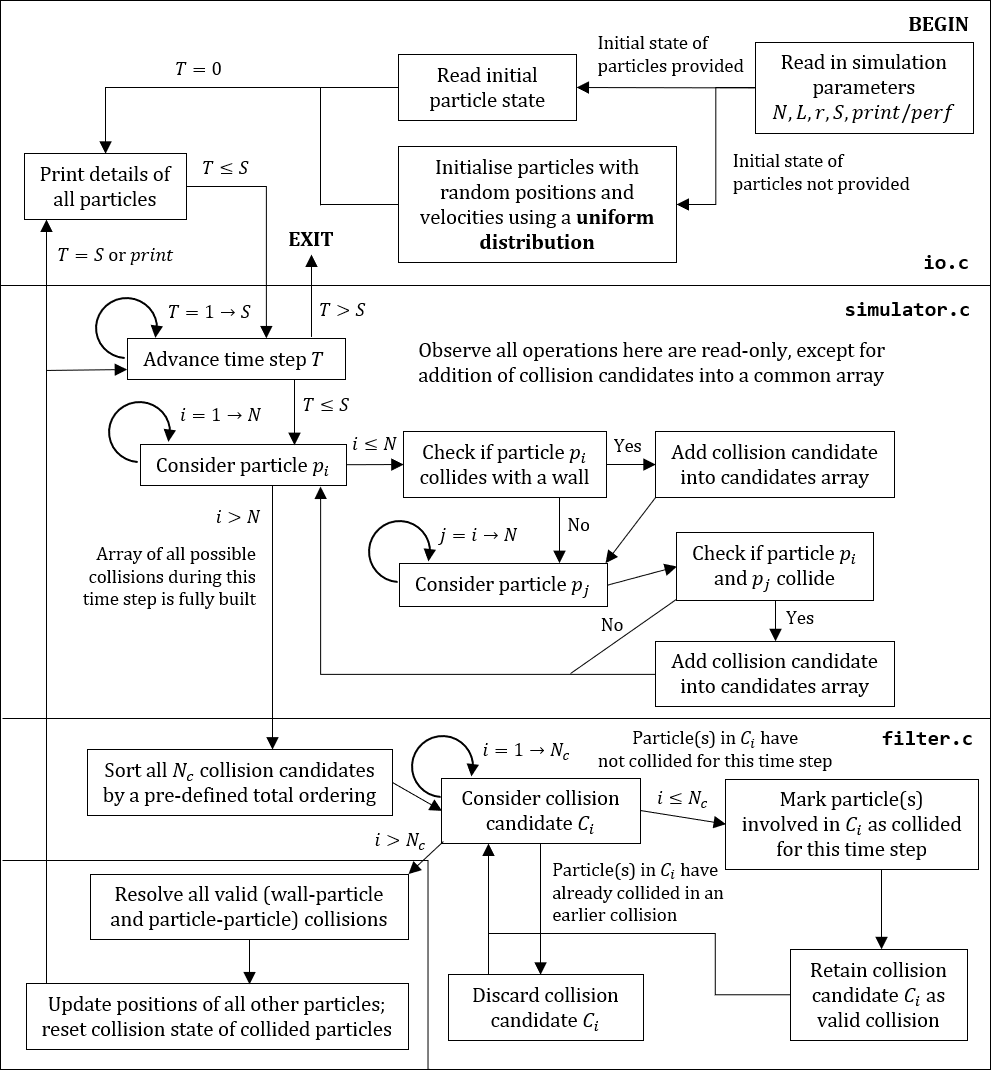
\includegraphics{chap1Flowchart}
\centering
\end{figure}

\pagebreak

\section{Implementation Assumptions and Details}

\subsection{Assumptions}

We make the following assumptions in our simulation.

\begin{enumerate}
	\item Even though the maximum initial velocity limit is $L/4$, we assume that the typical velocity of a particle is much less than this $\implies$ particles move only a small amount for each time step, hence for each particle $p_i$ and particle $p_j$, the probability of collision $P(p_i, p_j\ collide) \ll 1$ $\implies$ the total number of collisions per step $N_{collisions} = \Theta (N)$.
	\item A particle is involved in no more than one collision per time step.
	\begin{itemize}
		\item Implications
		\begin{enumerate}
			\item If a particle collides with a wall after any collision, it is placed at the wall at the end of that time step, ready to collide with the wall the next time step
			\item If particle $P$ collides with a particle $Q$ after any collision, it will phase through the particle $Q$ for the remainder of this time step, or will ignore $Q$ the next time step if they happen to overlap
		\end{enumerate}
	\end{itemize}
	\item All collisions between particles and with the wall are elastic (kinetic energy and momentum are conserved). 
	\item It is possible to fit all $N$ particles of radius $r$ into the square of length $L$ without overlapping.
	\begin{itemize}
		\item Implication
		\begin{enumerate}
			\item The simulation exits if one of these two conditions fail: $L < 2r$ (not possible to fit a single particle) or $Nr^2 > L^2$ (not possible to pack $N$ particles into a \ul{grid} in a square with area $L^2$)
		\end{enumerate}
	\end{itemize}
	\item The set of possible collisions $C$ satisfies a \textbf{total ordering}.
	\begin{itemize}
		\item Implication
		\begin{enumerate}
			\item For each time step $T$, it is possible to sort all collision candidates by this total ordering to determine which collisions should be prioritised over others.
		\end{enumerate}
	\end{itemize}
\end{enumerate}

\pagebreak

\subsection{Implementation Details}

\begin{enumerate}
	\item If the initial state of particles are not provided, particles are generated with initial random positions and velocities using a \textbf{uniform distribution}.
	\begin{enumerate}
		\item We use the pseudo-random number generator rand in the C library seeded with the number 3210.
		\item Particles are placed randomly in the square without overlapping.
	\end{enumerate}
	\item Each particle keeps track of its own state: $\textrm{ID}, x, y, v_x, v_y$.
	\item Our simulation has an additional parameter \texttt{SLOW\_FACTOR} in \texttt{simulator.c} that increases the granularity of the simulation for greater accuracy. \label{slow-factor-ref}
	\begin{enumerate}
		\item Setting \texttt{SLOW\_FACTOR} to an integer $>1$ slows the initial velocities of all particles by that factor. \texttt{SLOW\_FACTOR} should be set to a power of two to avoid introducing additional floating-point errors when dividing the particles’ velocities.
		\item The number of steps of the simulation is correspondingly multiplied by \texttt{SLOW\_FACTOR}, i.e. each original step now corresponds to \texttt{SLOW\_FACTOR} ``micro-steps".
	\end{enumerate}
	\item Collisions are of two types: either particle-wall collisions or particle-particle collisions. We describe a particle-wall collision as ($P$, \texttt{null}) and a particle-particle collision as ($P$, $Q$).
	\begin{enumerate}
		\item As particle-particle collisions are symmetric (i.e. $P$ collides with $Q$ $\iff$ $Q$ collides with $P$), we generate these collisions such that $P$ is the particle with lower integer ID.
	\end{enumerate}
	\item When sorting collision candidates with the C library function \texttt{qsort}, we enforce this total ordering in the function \texttt{cmpCollision}. For two collision candidates  $C_1$ and $C_2$,
	\begin{itemize}
		\item[$\blacksquare$] $C_1 < C_2$ if $C_1$ occurs before $C_2$
		\item[$\blacksquare$] If $C_1$ and $C_2$ occur at the same time
		\begin{itemize}
			\item[$\square$] $C_1 < C_2$ if the ID of $P$ in $C_1$ $<$ the ID of $P$ in $C_2$
			\item[$\square$] If $C_1$ and $C_2$ both involve the same particle $P$
				\begin{itemize}
					\item[$\blacksquare$] $C_1 < C_2$ if $C_1$ is a wall collision
					\item[$\blacksquare$] If $C_1$ and $C_2$ are both particle-particle collisions
						\begin{itemize}
							\item[$\square$] $C_1 < C_2$ if the ID of $Q$ in $C_1$ $<$ the ID of $Q$ in $C_2$
						\end{itemize}
				\end{itemize}
		\end{itemize}
	\end{itemize}
	\item For each particle in each time step, we check once if the particle collides with any of the four walls.
	\item (\textbf{Sequential and parallel-1}) All possible collision pairs are checked for each time step. The total number of collision checks performed is thus
	\begin{align*}
	N_{potential\ collisions} 	&= N_{wall-particle} + N_{particle-particle} \\
						&= N + \frac{N(N-1)}{2} \\
						&= \Theta (N^2)
	\end{align*}
	\item Particle-wall collisions are checked by solving the trajectory equation of a particle and the positions equations of the wall. The equations of the walls are $x = 0, x = L, y = 0, y = L$.
	\item \label{trajectory-calc} Particle-particle collisions are checked by solving trajectory equations of two particles during the given time step.
	
	Consider two particles $P$, $Q$ during a given time step $0 \leq \Delta t \leq 1$. From Pythagoras’ theorem, the distance between them is
	$$d = \sqrt{\left( \left( x_Q + v_{xQ} \Delta t \right) - \left( x_p + v_{xP} \Delta t \right) \right)^2 +
		\left( \left( y_Q + v_{yQ} \Delta t \right) - \left( y_p + v_{yP} \Delta t \right) \right)^2}$$
	or re-written in terms of deltas (differences in state)
	$$d = \sqrt{\left( \Delta x + \Delta v_x \Delta t \right)^2 +
		\left( \Delta y + \Delta v_y \Delta t \right)^2}$$
		
	The particles intersect when $d = 2r$, i.e. the particles touch at their circumference, hence by expanding and collecting terms we get the quadratic equation of form $A (\Delta t)^2 + B \Delta t + C = 0$,
	
	\begin{align*}
		\Delta x^2 + 2 \Delta x \Delta v_x \Delta t + \Delta v_x^2 (\Delta t)^2 + \Delta y^2 + 2 \Delta y \Delta v_y \Delta t + \Delta v_y^2 (\Delta t)^2 &= (2r)^2 \\
		\implies (\Delta v_x^2 + \Delta v_y^2) (\Delta t)^2 + (2 \Delta x \Delta v_x + 2 \Delta y \Delta v_y) \Delta t + (\Delta x^2 + \Delta y^2 - 4r^2) &= 0
	\end{align*}
	
	We observe that $A = (\Delta v_x^2 + \Delta v_y^2) > 0$ and thus the curve $y = d(\Delta t)$ is concave up. The discriminant for this quadratic equation, $B^2 - 4AC$, is
	$$\textrm{discriminant} = (2 \Delta x \Delta v_x + 2 \Delta y \Delta v_y)^2 - 4(\Delta v_x^2 + \Delta v_y^2)(\Delta x^2 + \Delta y^2 - 4r^2)$$
	
	If this discriminant is $\geq 0$, then the particles collide for some value of $\Delta t$, and we solve for this $\Delta t$. There are two possible roots,
	$$\Delta t = \frac{-B \pm \sqrt{\textrm{discriminant}}}{2A}$$
	
	Since the quadratic curve is concave up, we only compute and examine the first root (when the particles are approaching each other). This is
	$$\Delta t = \frac{-B - \sqrt{\textrm{discriminant}}}{2A}$$
	
	If $0 \leq \Delta t \leq 1$, then particles $P$, $Q$ collide during this time step.
	
	Note that, it is possible for $\Delta t < 0$ - this corresponds to cases where particles are overlapping from a previous step. We do not consider these as collisions in the current step and let these two particles phase through each other.
\end{enumerate}

\pagebreak

\section{Parallelisation Strategy}

A large part of the simulation is highly sequential in nature and not amenable to parallelisation. For each simulation step, all collision candidates have to be generated first before sorting is performed, then followed by filtering, before the collisions can be resolved in a parallel manner. \\

From our sequential implementation, there were some loops and independent function calls that were potentially amenable to parallelisation with OpenMP. \\

Decisions regarding parallelisation and synchronisation constructs are detailed below, in the order they are encountered in the diagram in Chapter 1.

\begin{center}
\begin{tabular}{ | m{5em} | m{33em} | } 
\hline
\textbf{File, Line} & \bt{random.c: 8-13} \\ \hline
\textbf{Program Fragment} &
\begin{minted}{c}
for (int i = 0; i < n; i++) {
    // Build N particle structs and update pointers
}
\end{minted}
\\ \hline
\textbf{Decision} &
This loop can be safely parallelised with \bt{\#pragma omp for}, as the pointer to each particle is written to different indices of the array \textbf{particleArray}. We did \ul{not parallelise this loop} however as the overhead of parallelisation is much greater than the benefit.
\\ \hline
\end{tabular}
\end{center}

\begin{center}
\begin{tabular}{ | m{5em} | m{33em} | } 
\hline
\textbf{File, Line} & \bt{random.c: 37-55} \\ \hline
\textbf{Program Fragment} &
\begin{minted}{c}
for (int i = 0; i < n; i++) {
    // Repeatedly place particles without overlapping
}
\end{minted}
\\ \hline
\textbf{Decision} &
This loop \ul{cannot be safely parallelised}, since each particle placed randomly in the square needs to check if it overlaps with any of the particles that were previously placed.
\\ \hline
\end{tabular}
\end{center}

\begin{center}
\begin{tabular}{ | m{5em} | m{33em} | } 
\hline
\textbf{File, Line} & \bt{random.c: 73-80} \\ \hline
\textbf{Program Fragment} &
\begin{minted}{c}
for (int i = 0; i < n; i++) {
    // Generate random velocities
}
\end{minted}
\\ \hline
\textbf{Decision} &
This loop can be safely parallelised with \bt{\#pragma omp for}, since each iteration of the loop updates different indices of the random velocity array. We did \ul{not parallelise this loop} due to overhead.
\\ \hline
\end{tabular}
\end{center}

\begin{center}
\begin{tabular}{ | m{5em} | m{33em} | } 
\hline
\textbf{File, Line} & \bt{io.c: 47-59} \\ \hline
\textbf{Program Fragment} &
\begin{minted}{c}
for (int i = 0; i < n; i++) {
    // Print details of every particle for a given step
}
\end{minted}
\\ \hline
\textbf{Decision} &
This loop \ul{cannot be parallelised}. Print statements are not atomic, and attempting to parallelise this only messes up the ordering of the printed output to amusing effect.
\\ \hline
\end{tabular}
\end{center}

\begin{center}
\begin{tabular}{ | m{5em} | m{33em} | } 
\hline
\textbf{File, Line} & \bt{simulator.c: 55-59} \\ \hline
\textbf{Program Fragment} &
\begin{minted}{c}
for (int i = 0; i < n; i++) {
    // Initialise collision state of each particle to false
}
\end{minted}
\\ \hline
\textbf{Decision} &
This loop can be safely parallelised with \bt{\#pragma omp for}, since each iteration of the loop updates different indices of the collision state array. We did \ul{not parallelise this loop} however due to overhead.
\\ \hline
\end{tabular}
\end{center}

\begin{center}
\begin{tabular}{ | m{5em} | m{33em} | } 
\hline
\textbf{File, Line} & \bt{simulator.c: 62-131} \\ \hline
\textbf{Program Fragment} &
\begin{minted}{c}
for (int step = 1; step <= s; step++) {
    // Simulate step T
}
\end{minted}
\\ \hline
\textbf{Decision} &
This loop is inherently \ul{unparallelisable}. Steps of a simulation are sequential in nature since the $(n+1)$-th step is dependent on the state of the $n$-th step.
\\ \hline
\end{tabular}
\end{center}

\begin{center}
\begin{tabular}{ | m{5em} | m{33em} | } 
\hline
\textbf{File, Line} & \bt{simulator.c: 69-106} \\ \hline
\textbf{Program Fragment} &
\begin{minted}{c}
#pragma omp parallel
{
    #pragma omp for schedule(dynamic, 1)
    for (int p = 0; p < n; p++) {
        // Check if this particle p will colide with a wall
        // For every particle q of greater ID, check if p, q
        // will collide
    }
}
\end{minted}
\\ \hline
\textbf{Decision} &
We opted to \ul{parallelise this loop}, since checking all $\Theta(N^2)$ potential collisions is expensive. However, each iteration of the outer loop (for a particle $P$) performs a different number of checks on other particles $Q$. Thus, we opted to use dynamic scheduling with chunk size 1 - which uses an internal work queue to assign threads 1 outer loop iteration each time they are finished with the previous iteration. Despite the extra overhead from the queue, this minimises total execution time relative to other scheduling policies since it distributes work equitably amongst the threads. All threads are implicitly synchronised at the end of the \bt{\#pragma omp for} construct, before the simulation proceeds.
\\ \hline
\end{tabular}
\end{center}

\begin{center}
\begin{tabular}{ | m{5em} | m{33em} | } 
\hline
\textbf{File, Line} & \bt{simulator.c: 81-87, 96-102} \\ \hline
\textbf{Program Fragment} &
\begin{minted}{c}
#pragma omp critical
{
    // Add a new collision candidate to an array
    // Increment number of collision candidates for that step
}
\end{minted}
\\ \hline
\textbf{Decision} &
In the parallelised for loop for generating collision candidates, race conditions may occur when multiple threads attempt to add a new collision candidate to the \bt{cs} array and increment \bt{numCollisions}. Therefore, we protected both critical sections (for particle-wall and particle-particle collisions) within a \bt{\#pragma omp critical} construct to prevent concurrent modification.
\\ \hline
\end{tabular}
\end{center}

\begin{center}
\begin{tabular}{ | m{5em} | m{33em} | } 
\hline
\textbf{File, Line} & \bt{filter.c: 12-34} \\ \hline
\textbf{Program Fragment} &
\begin{minted}{c}
for (int curIndex = 0; curIndex < *numCollisions; curIndex++) {
    // Filters array of collision candidates down to
    // only valid collisions
}
\end{minted}
\\ \hline
\textbf{Decision} &
This loop \ul{cannot be parallelised}. For a given step, collision candidates need to be processed by their total ordering, since accepting a collision as valid may invalidate some of the later collision candidates (as particles are involved in at most one collision per step).
\\ \hline
\end{tabular}
\end{center}

\begin{center}
\begin{tabular}{ | m{5em} | m{33em} | } 
\hline
\textbf{File, Line} & \bt{kinematics.c: 8-20} \\ \hline
\textbf{Program Fragment} &
\begin{minted}{c}
collision_t* curCollision
#pragma omp parallel private(curCollision)
{
    // Compute chunk size
    #pragma omp for schedule(static, chunk_size)
    for (int i = 0; i < *numCollisions; i++) {
        // Resolve each valid collision after sorting and
        // filtering of collision candidates
        // Update state of particles involved
    }
}
\end{minted}
\\ \hline
\textbf{Decision} &
A particle can only be involved in at most one valid collision. Thus, parallelising this loop can be done safely since at most one thread will be updating the state of any given particle. Since resolving collisions is computationally expensive, we \ul{parallelised this loop}, using static scheduling with equal chunk sizes to map loop iterations to threads.
\\ \hline
\end{tabular}
\end{center}

\begin{center}
\begin{tabular}{ | m{5em} | m{33em} | } 
\hline
\textbf{File, Line} & \bt{kinematics.c: 27-40} \\ \hline
\textbf{Program Fragment} &
\begin{minted}{c}
for (int i = 0; i < n; i++) {
    // For a given time step, update position of all particles
    // not involved in a collision
    // Also resets state of collided particles
}
\end{minted}
\\ \hline
\textbf{Decision} &
This loop can be safely parallelised with \bt{\#pragma omp for}, as each particle’s state is only updated by one thread when parallelised. We did \ul{not parallelise this loop} however as the overhead of parallelisation is much greater than the benefit.
\\ \hline
\end{tabular}
\end{center}

\pagebreak

\section{Test Conditions and Testcases}

\subsection{Test Setup}

Benchmarking of our sequential, parallel and early-pruning implementations were done on the same lab machines with aid of a Python script to generate input files (\texttt{generateTestcases.py}) and a Bash script to execute and log output for each testcase. These files can be found in the \texttt{<impl>BatchRuns} sub-folder of the respective implementation (under \texttt{/code/<impl>/}). \\

The Intel i7-7700K node tested was \ul{soctf-pdc-001} and the Intel Xeon Silver 4114 node tested was \ul{soctf-pdc-010}. Each testcase was run five times and the fastest execution time was retained as the datapoint for that testcase. \\

To replicate our results for a given implementation, compile all files in that folder with \bt{gcc *.h} followed by \bt{gcc -fopenmp *.c -lm}. Then, execute the corresponding Bash script in the associated \texttt{<impl>BatchRuns} sub-folder.

\subsection{Random Testcases}

For benchmarking, testcases ran in \textit{perf} mode and the initial states of particles were not provided. Variables of the simulation were adjusted for each testcase. \\

The simulation parameters of the default testcase are
\begin{itemize}
	\item $N = 1000, L=20000, r=1, S=1000$
\end{itemize}

The testcases that were executed for each implementation are as follows. 
\begin{enumerate}
	\item Sequential implementation
	\begin{itemize}
		\item Varying $N$ only: $N = 250, 375, 500, 750, 1500, 2000$
		\item Varying $L$ only: $L = 5000, 7500, 15000, 20000$
		\item Varying $r$ only: $r = 1, 2, 3, 4, 6, 8, 16$
		\item Varying $S$ only: $S = 250, 375, 500, 750, 1500, 2000$
	\end{itemize}
	
	\item Parallel implementation
	\begin{itemize}
		\item $T$ = number of OpenMP threads
		\item Varying both $N$ and $T$ together
		\begin{itemize}
			\item $N = 250, 500, 1000, 2000$
			\item $T = 1, 2, 4, 6, 7, 8, 9, 10, 12, 16, 19, 20, 21, 24, 28, 32, 40, 64$
		\end{itemize}
	\end{itemize}
\end{enumerate}

\pagebreak

\subsection{Special Testcases}

In addition to the random testcases, we designed a few additional special testcases to assert correctness of our simulator, alongside an extra Python script (in folder \texttt{/scripts}: \texttt{generateAnimation.py}) to visualise the simulation output. We provided the \texttt{.GIF} visualisations for each of these testcases. \\

Each of these testcases are named accordingly, and should be run with \texttt{SLOW\_FACTOR} set to a power of two (we recommend 16) for accuracy. Running these testcases with other values of \texttt{SLOW\_FACTOR} may lead to different results due to floating-point errors or insufficient granularity of simulation. \\

These testcases are as follows.

\begin{itemize}
	\item \texttt{cradle.in} - a horizontal row of particles that behaves like Newton’s cradle, endlessly bouncing between two walls
	\item \texttt{cross.in} - two particles bouncing between opposite diagonals of the square, without ever colliding
	\item \texttt{diagonalLine.in} - a diagonal row of particles bouncing from left to right, with glancing collisions
	\item \texttt{square.in} - four particles colliding at the same time at the centre; all four particles are deflected exactly at right angles from their initial trajectory
	\item \texttt{triangle.in} - three particles colliding at the same time, with resolution to prioritise the collision between the pair of particles with lowest ID
\end{itemize}

\pagebreak

\section{Execution Time Results}

All plots were generated with the help of R. The raw data from the \bt{perf stat} command is available in the submission as \texttt{.csv} files in \texttt{/data/sequential} and \texttt{/data/sequentialVsParallel}. Some of the plots are not reproduced here for brevity.

\subsection{Sequential Implementation}

\begin{figure}[H]
    \centering
    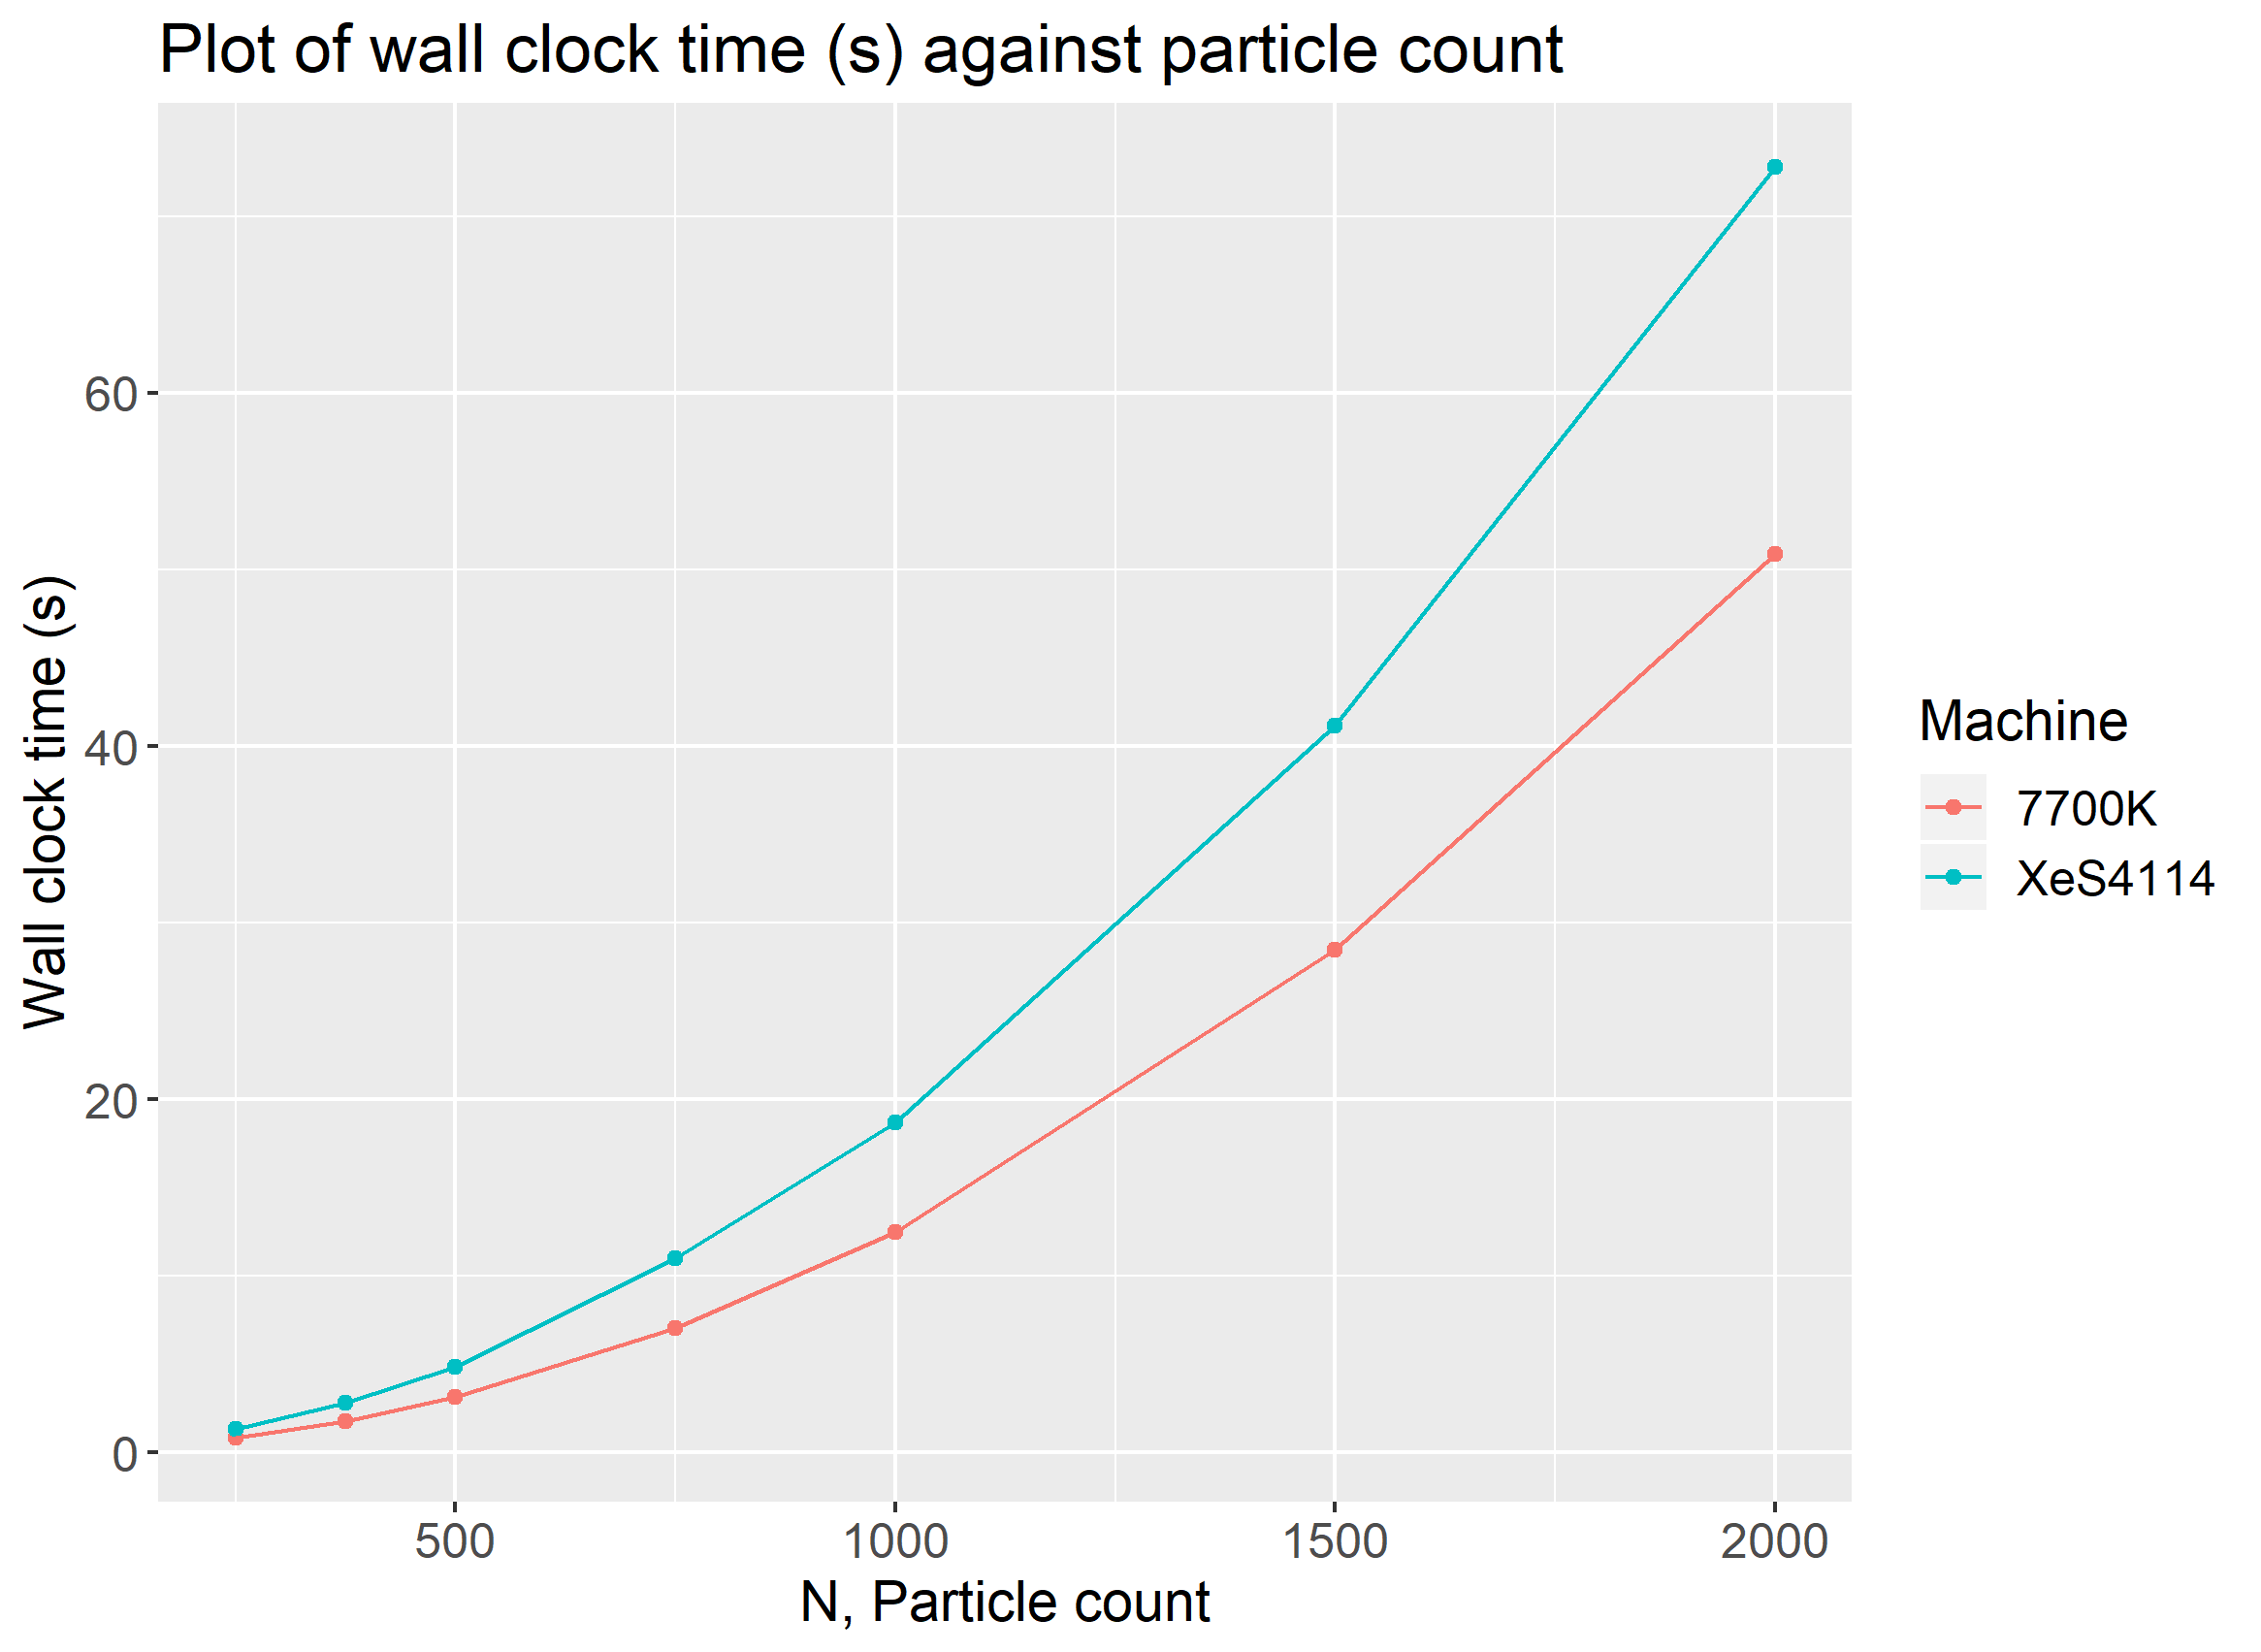
\includegraphics[width=0.75\textwidth]{seq-varyN}
    \caption{Plot of execution time against particle count, $N$}
    \label{fig:seq-varyN}
\end{figure}

\begin{figure}[H]
    \centering
    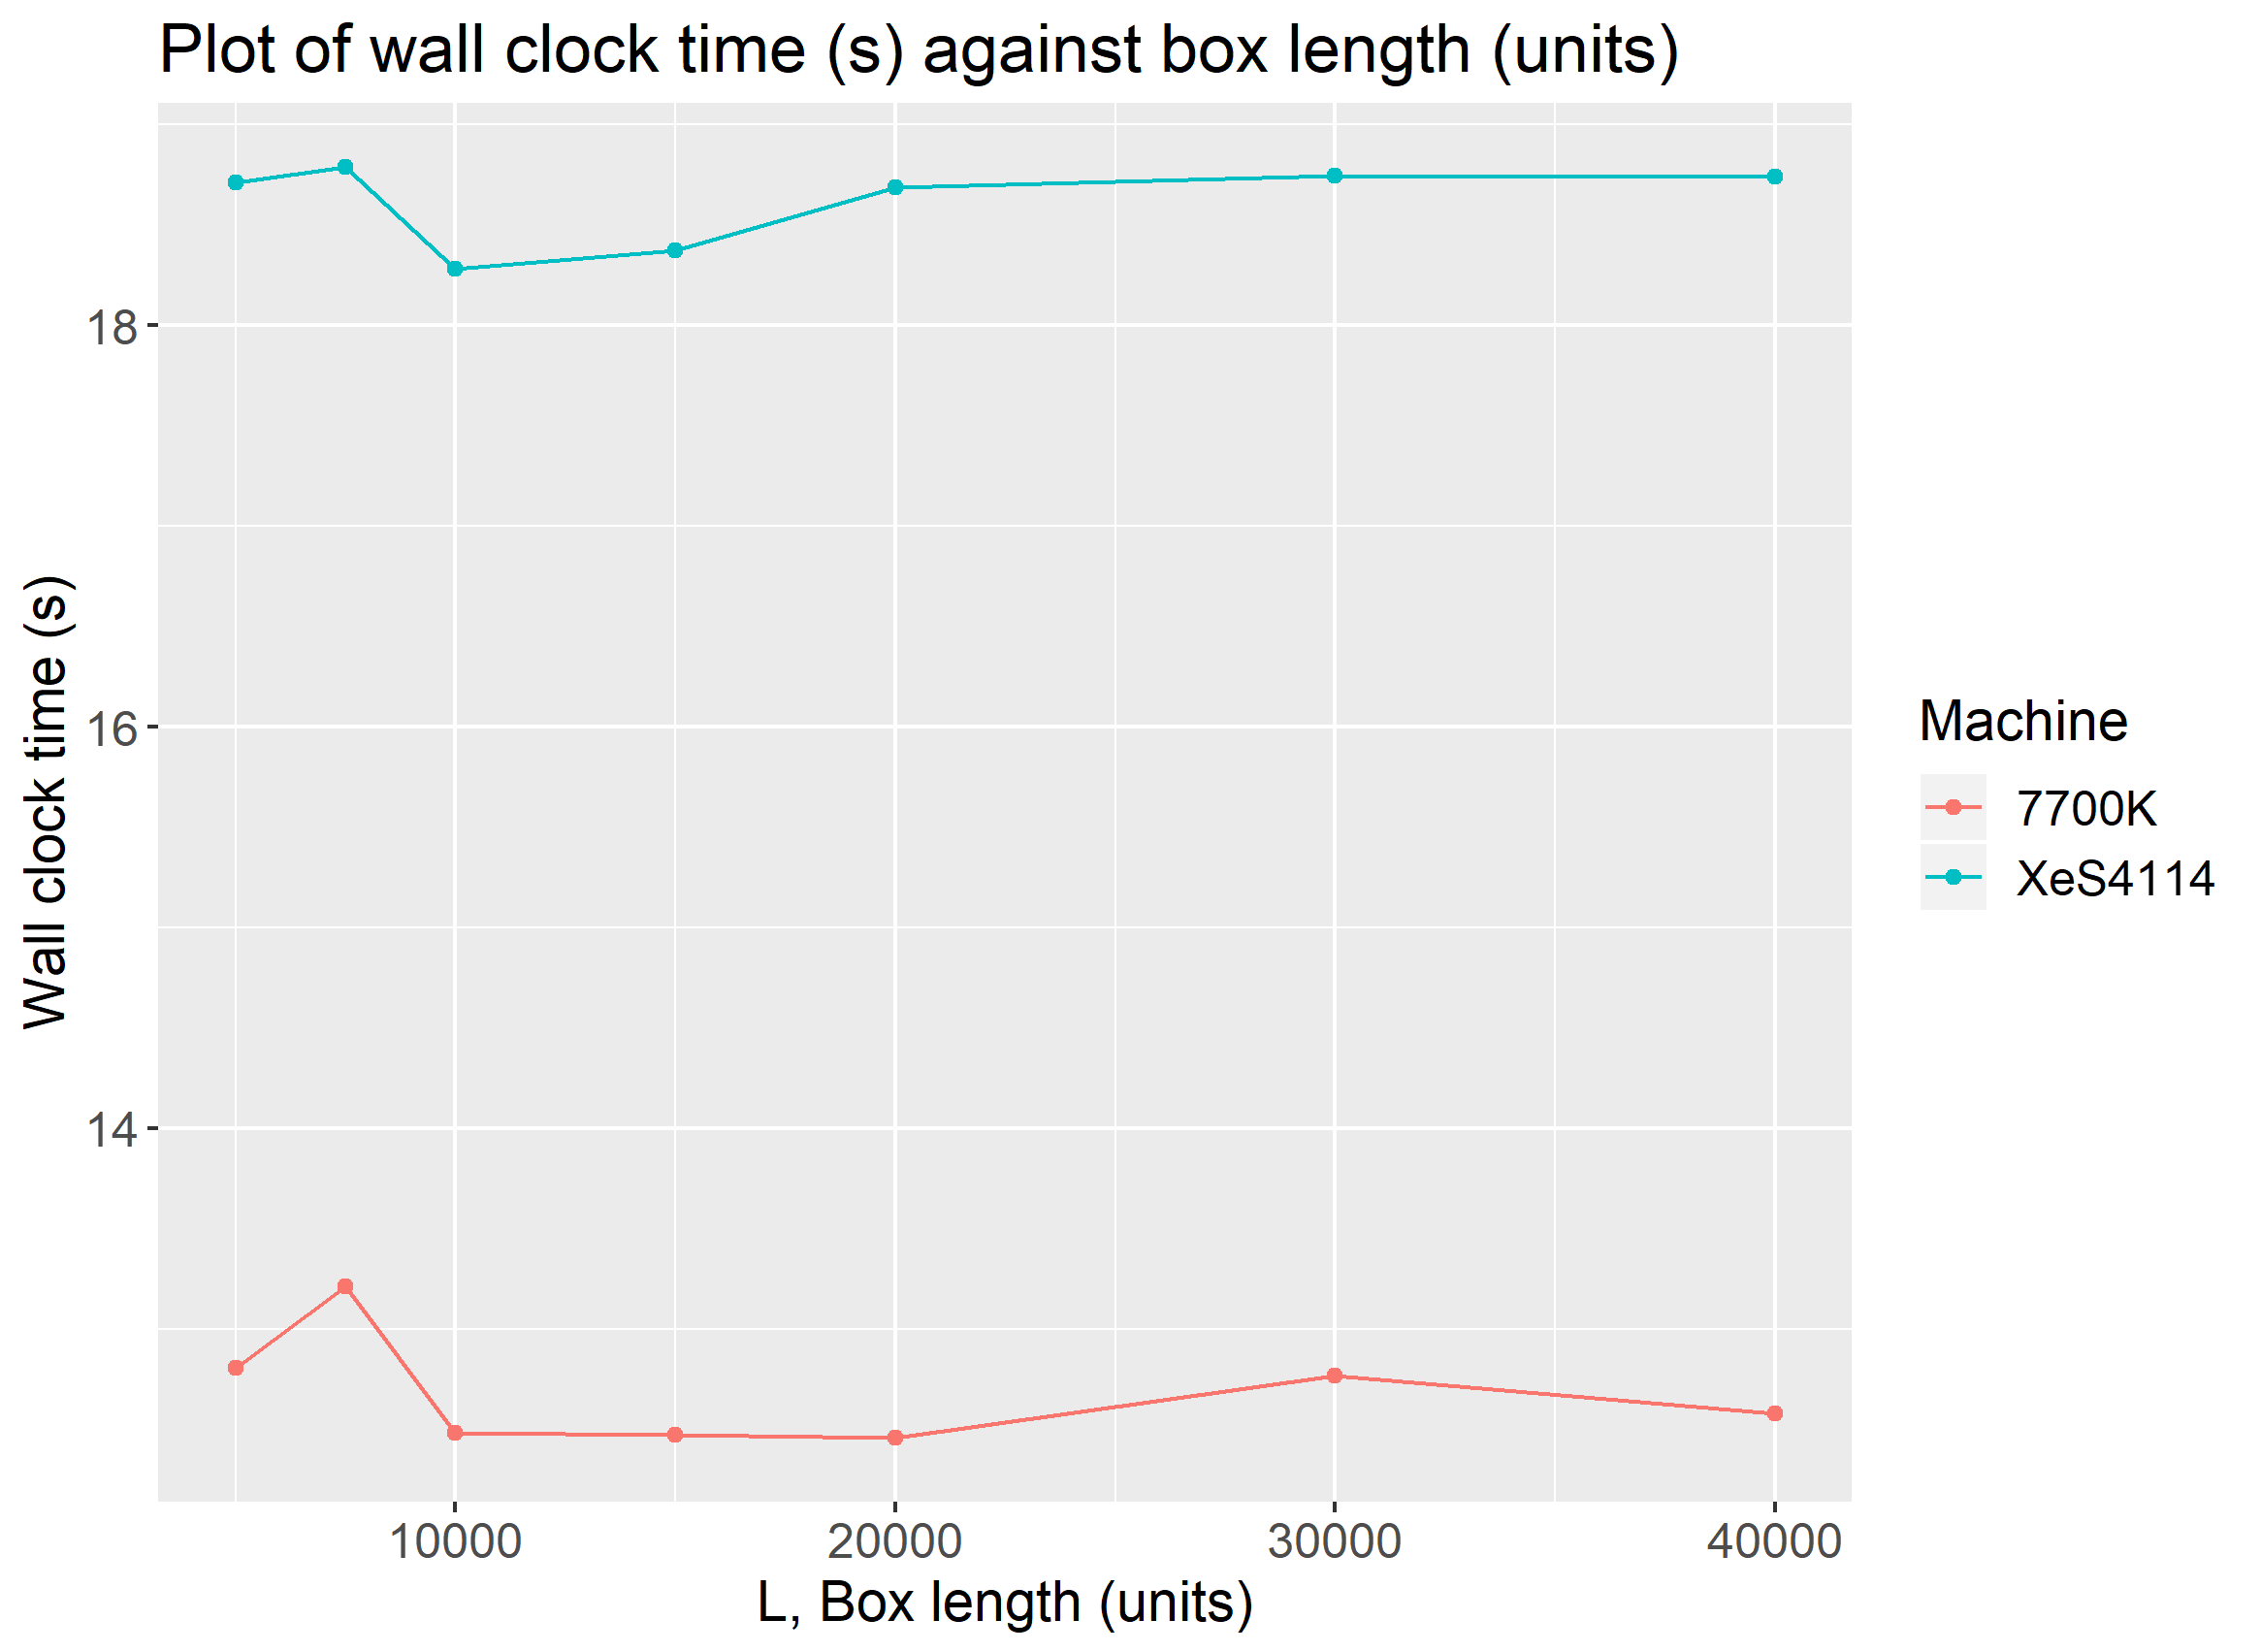
\includegraphics[width=0.75\textwidth]{seq-varyL}
    \caption{Plot of execution time against box length, $L$}
    \label{fig:seq-varyL}
\end{figure}

\begin{figure}[H]
    \centering
    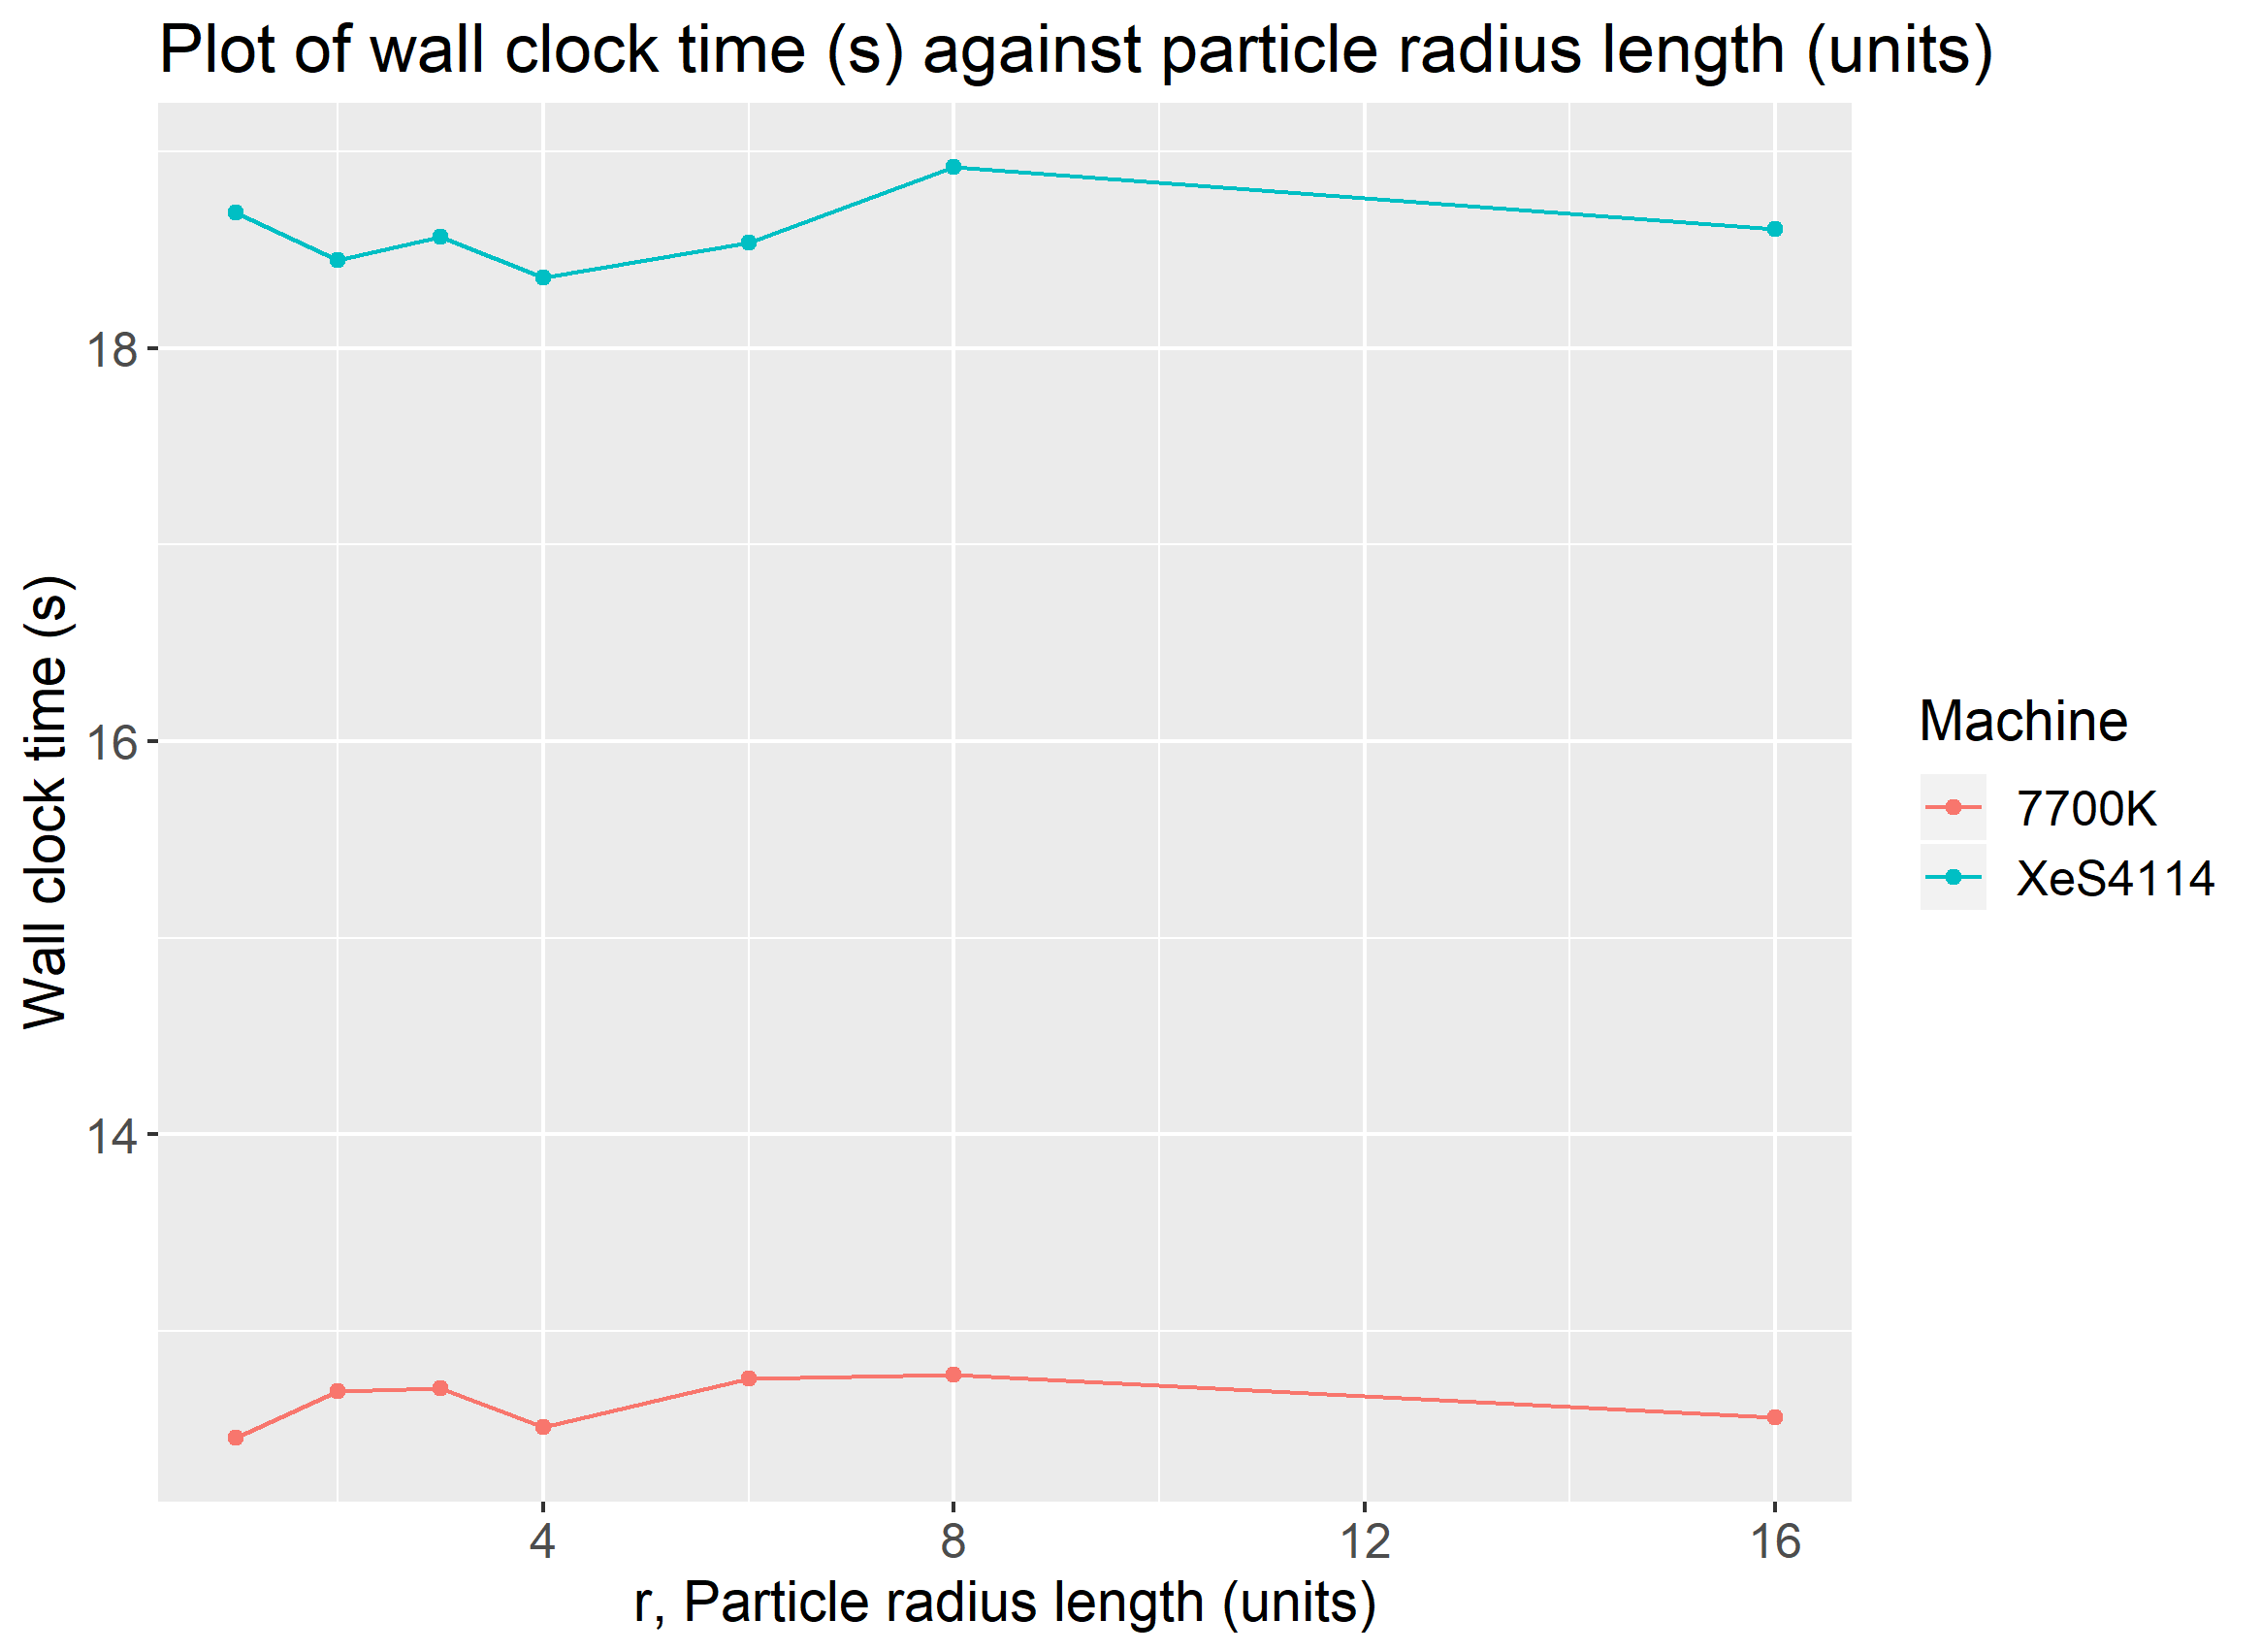
\includegraphics[width=0.75\textwidth]{seq-varyR}
    \caption{Plot of execution time against particle radius, $r$}
    \label{fig:seq-varyR}
\end{figure}

\begin{figure}[H]
    \centering
    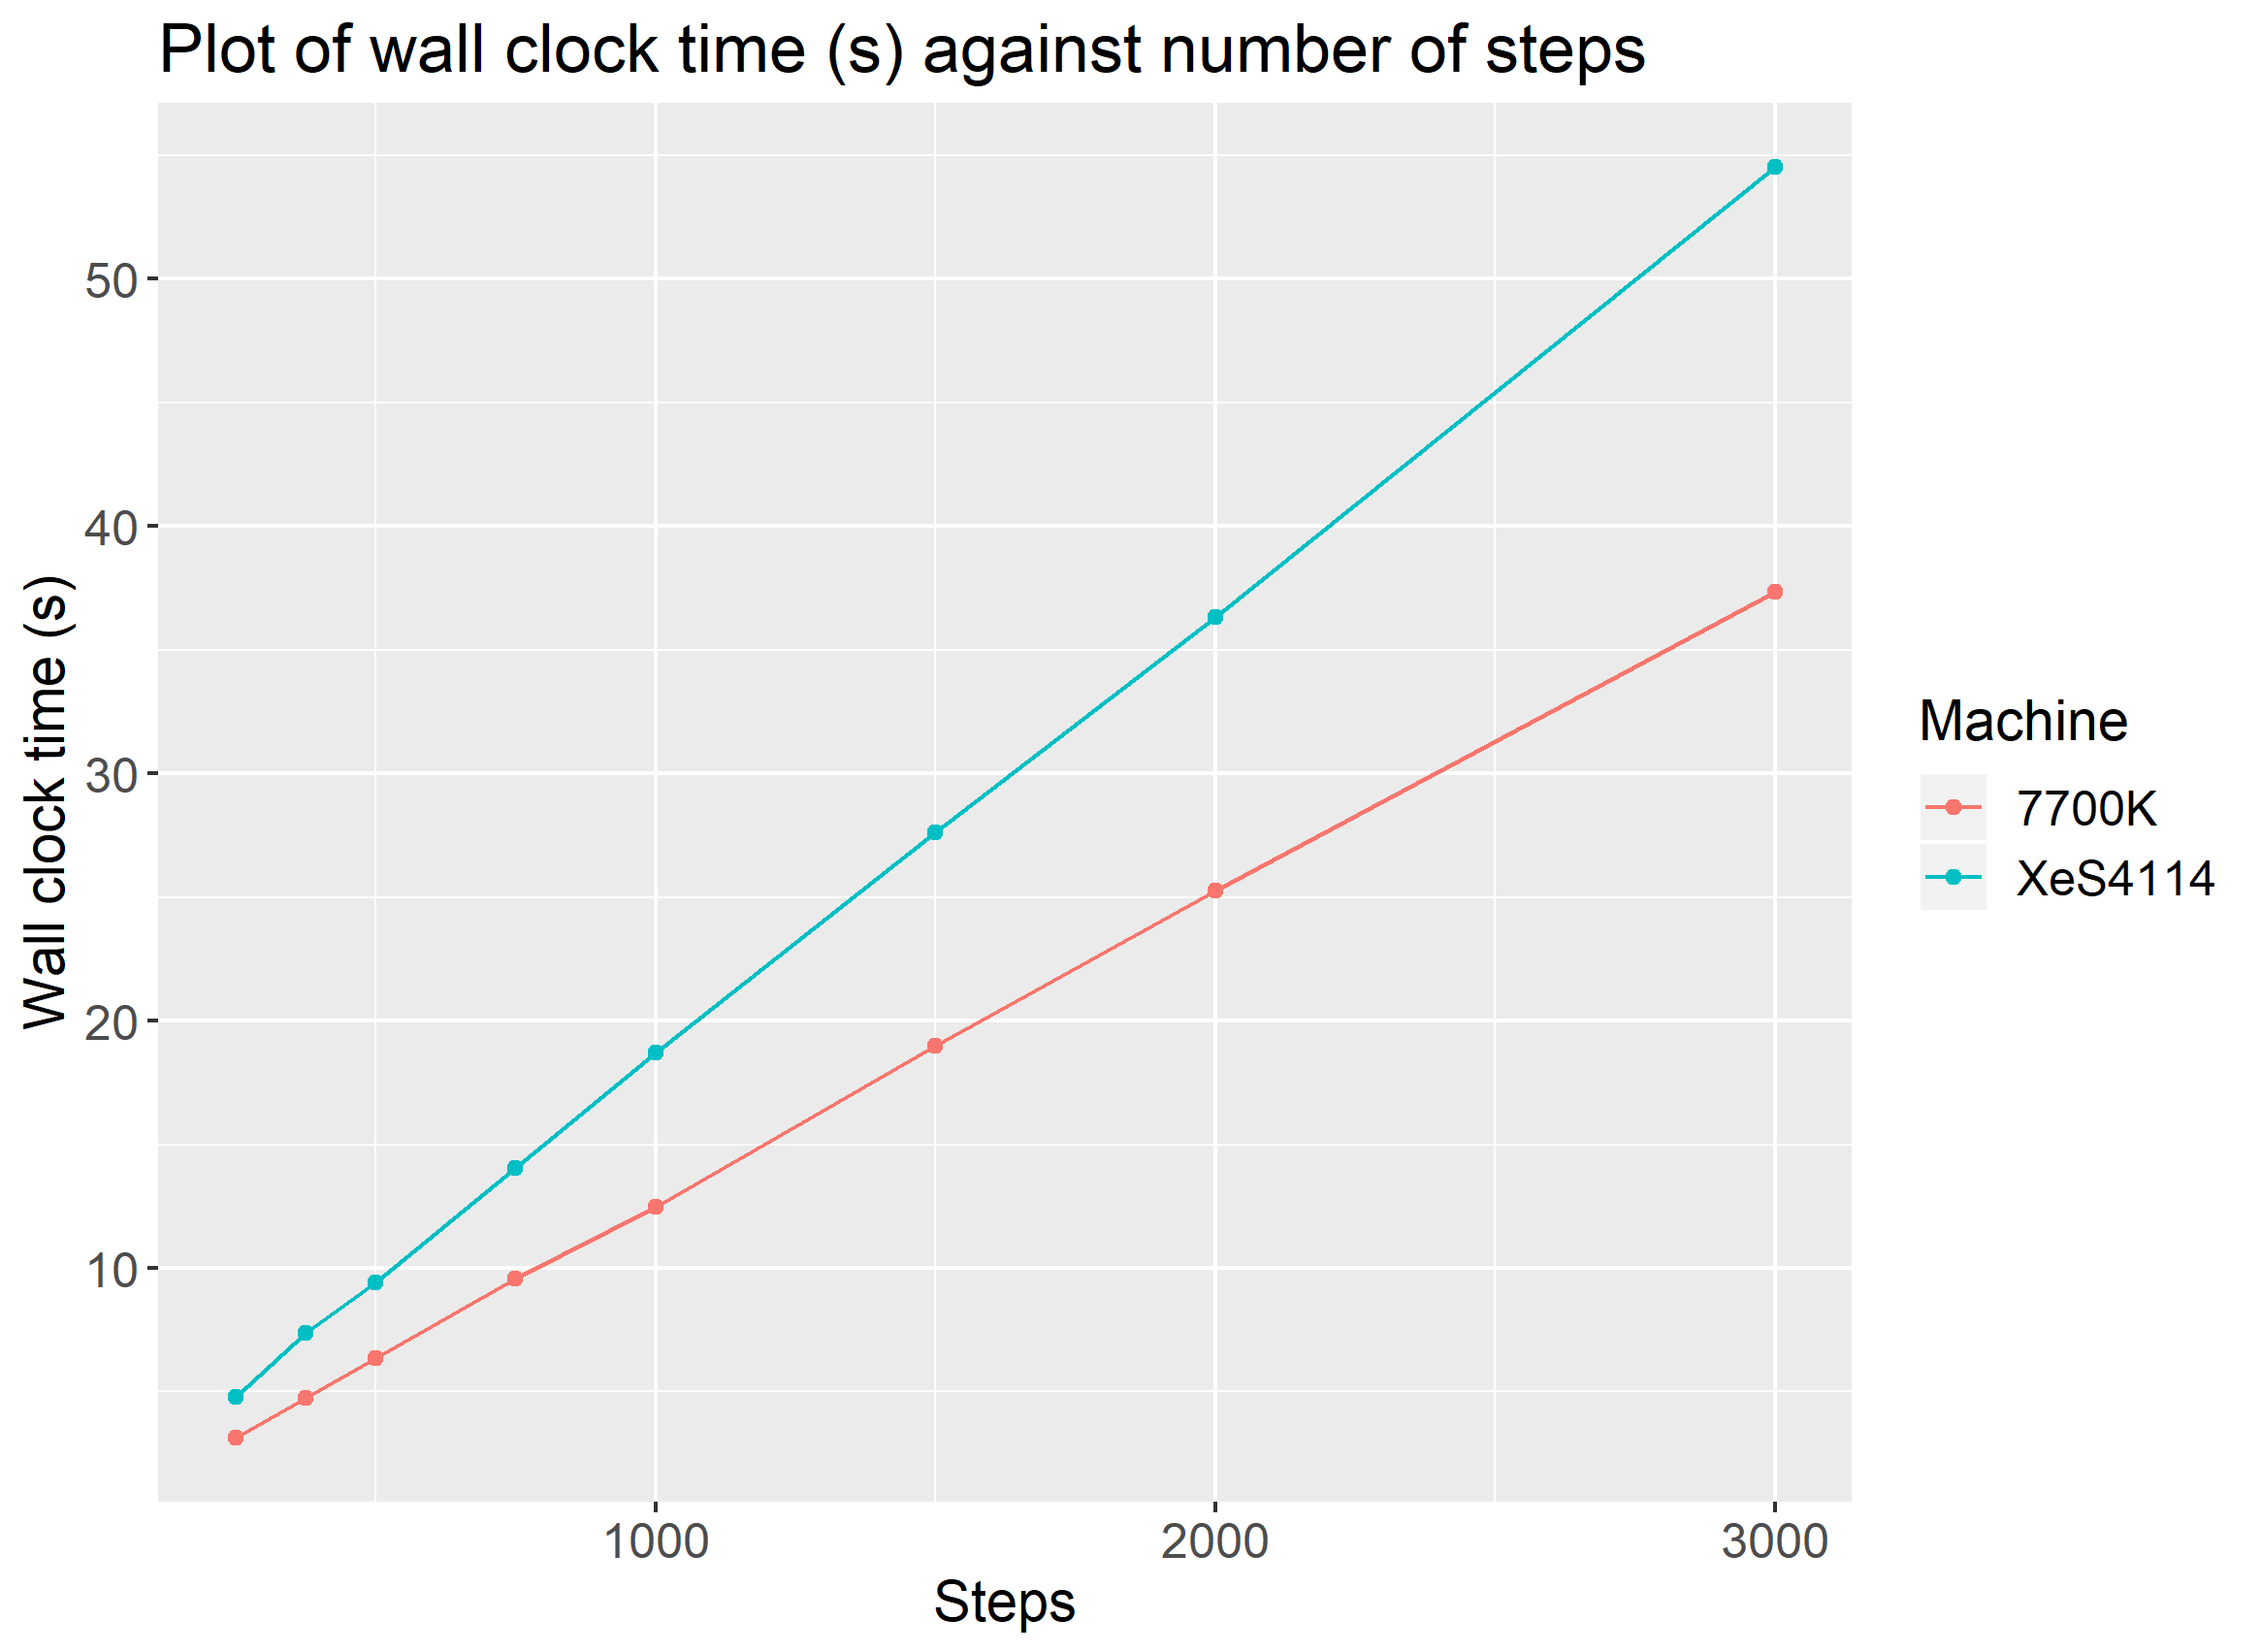
\includegraphics[width=0.75\textwidth]{seq-varySteps}
    \caption{Plot of execution time against number of steps, $S$}
    \label{fig:seq-varySteps}
\end{figure}

\pagebreak

\subsection{Parallel Implementation}

\begin{figure}[H]
    \centering
    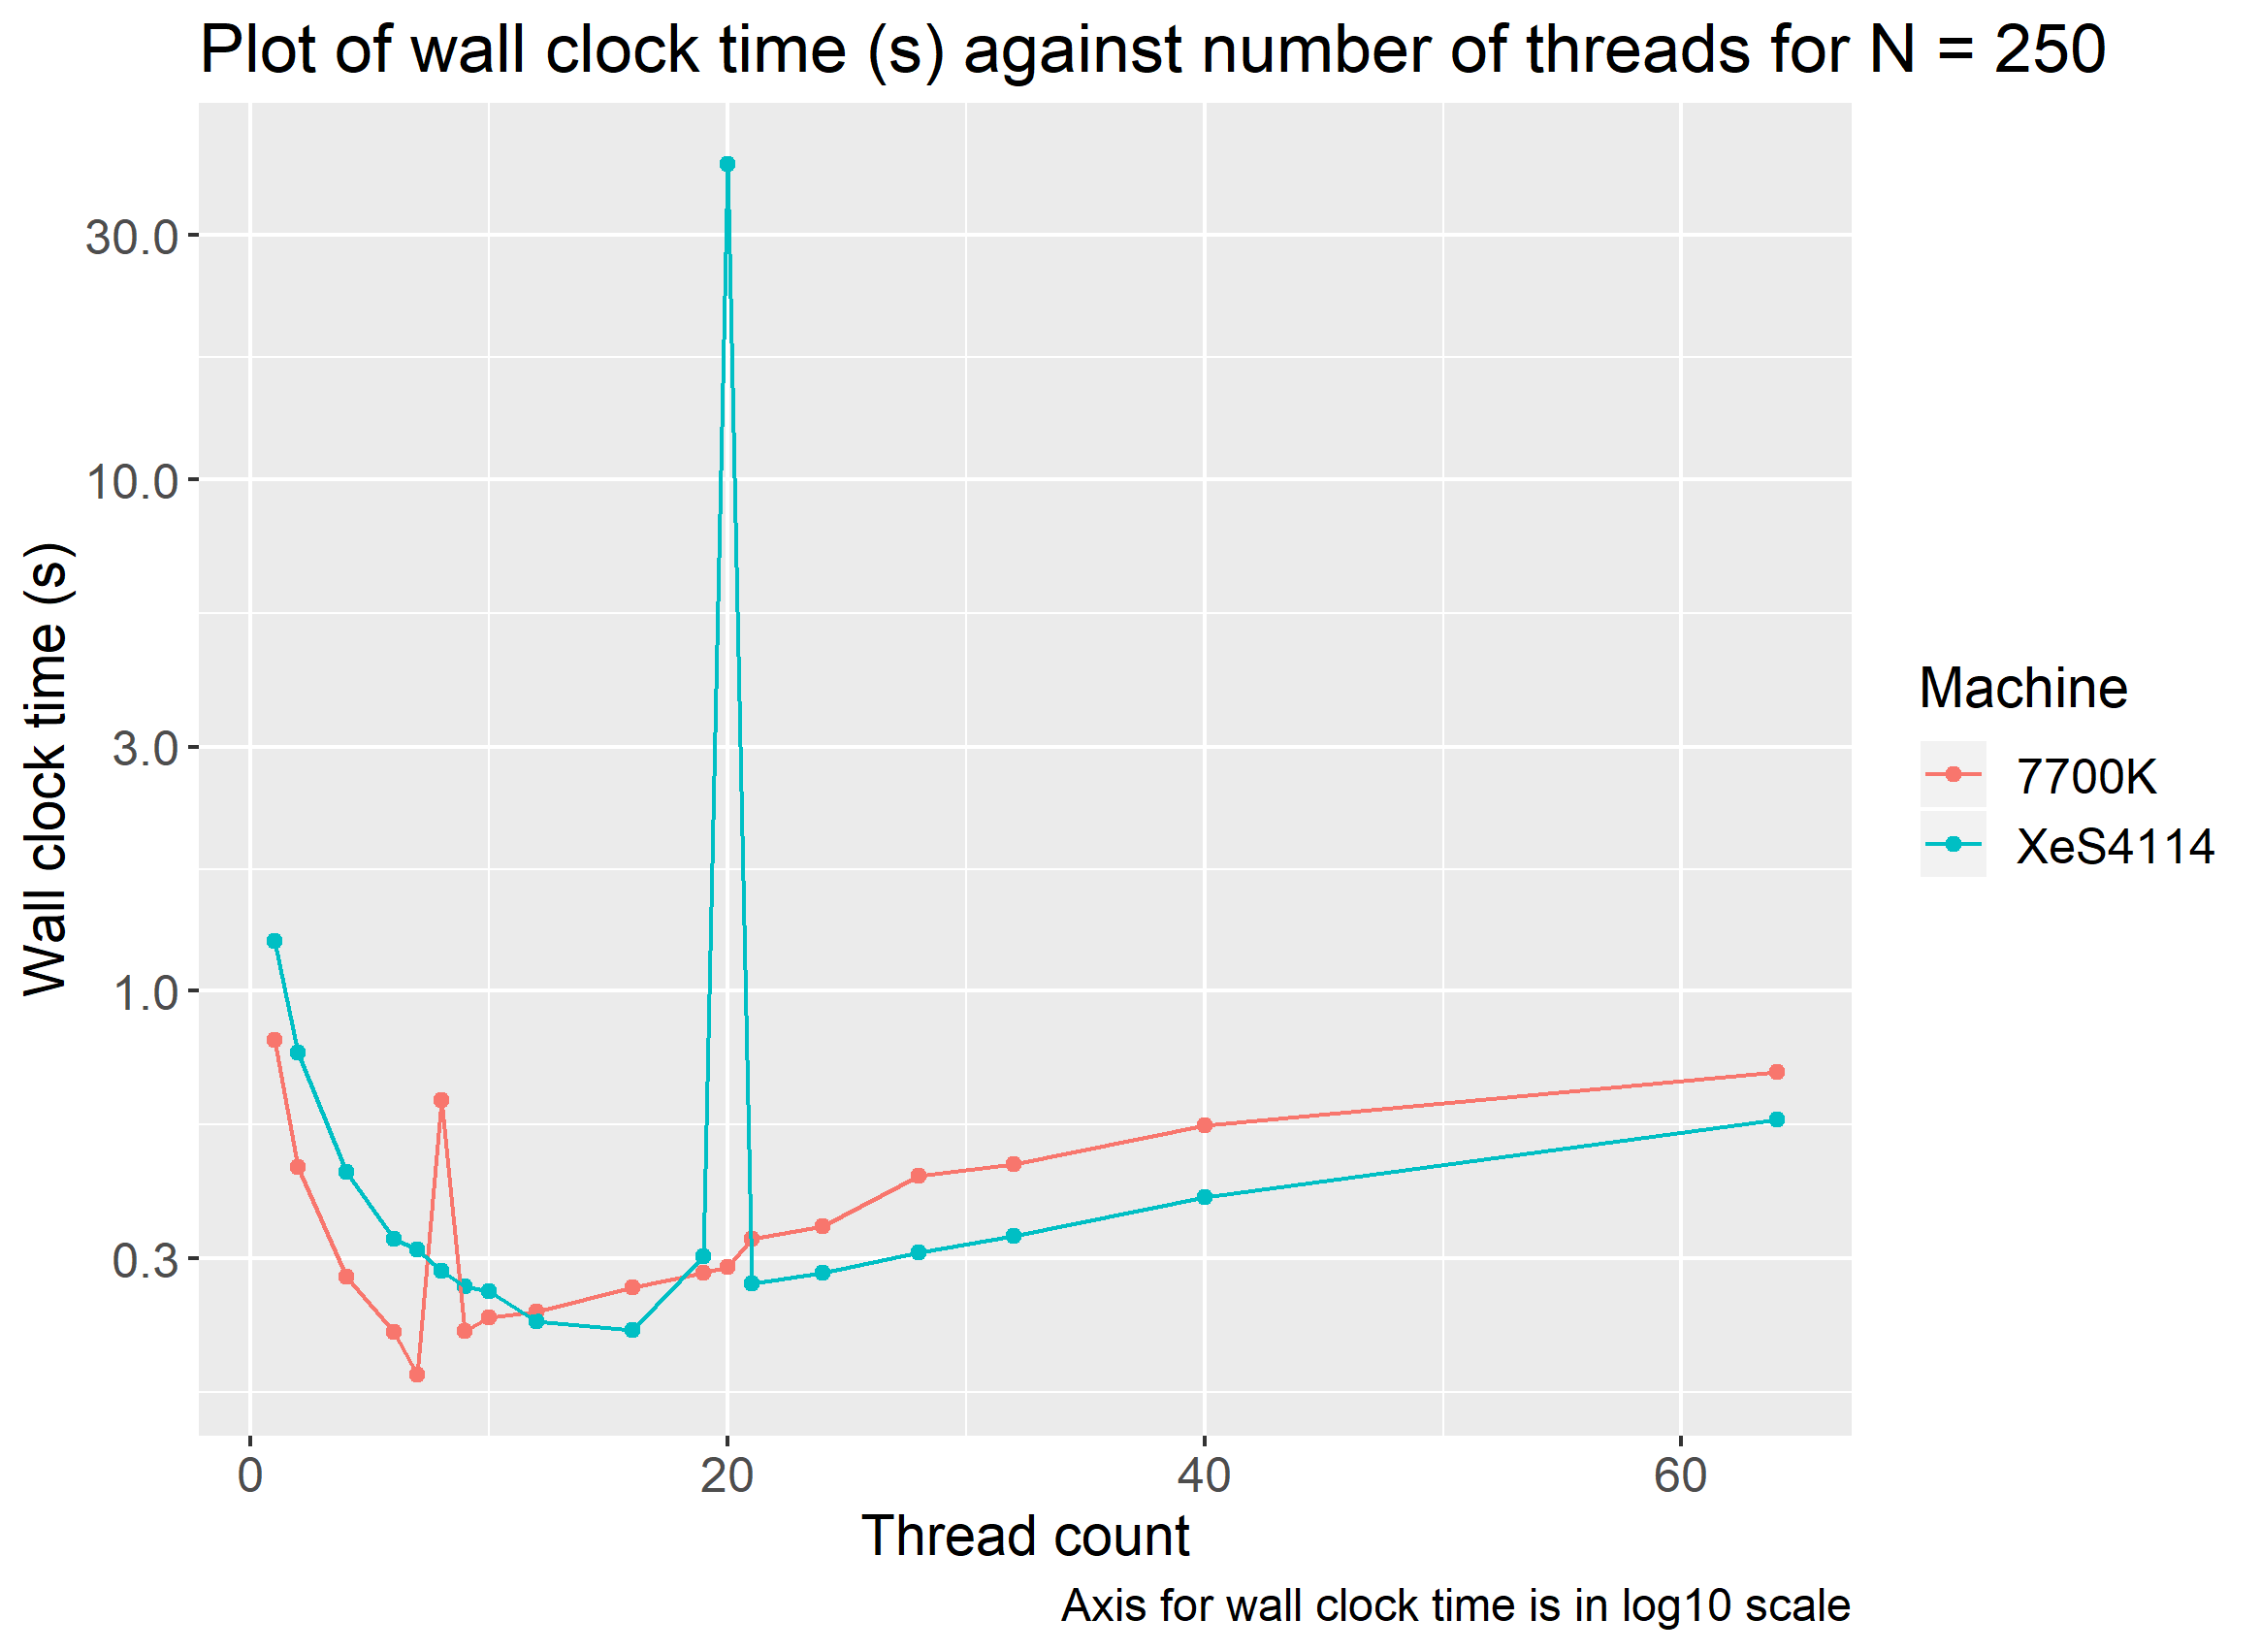
\includegraphics[width=0.75\textwidth]{par-250N-varyThreads}
    \caption{Plot of execution time against number of threads $T$ for $N = 250$}
    \label{fig:par-250N-varyThreads}
\end{figure}

\begin{figure}[H]
    \centering
    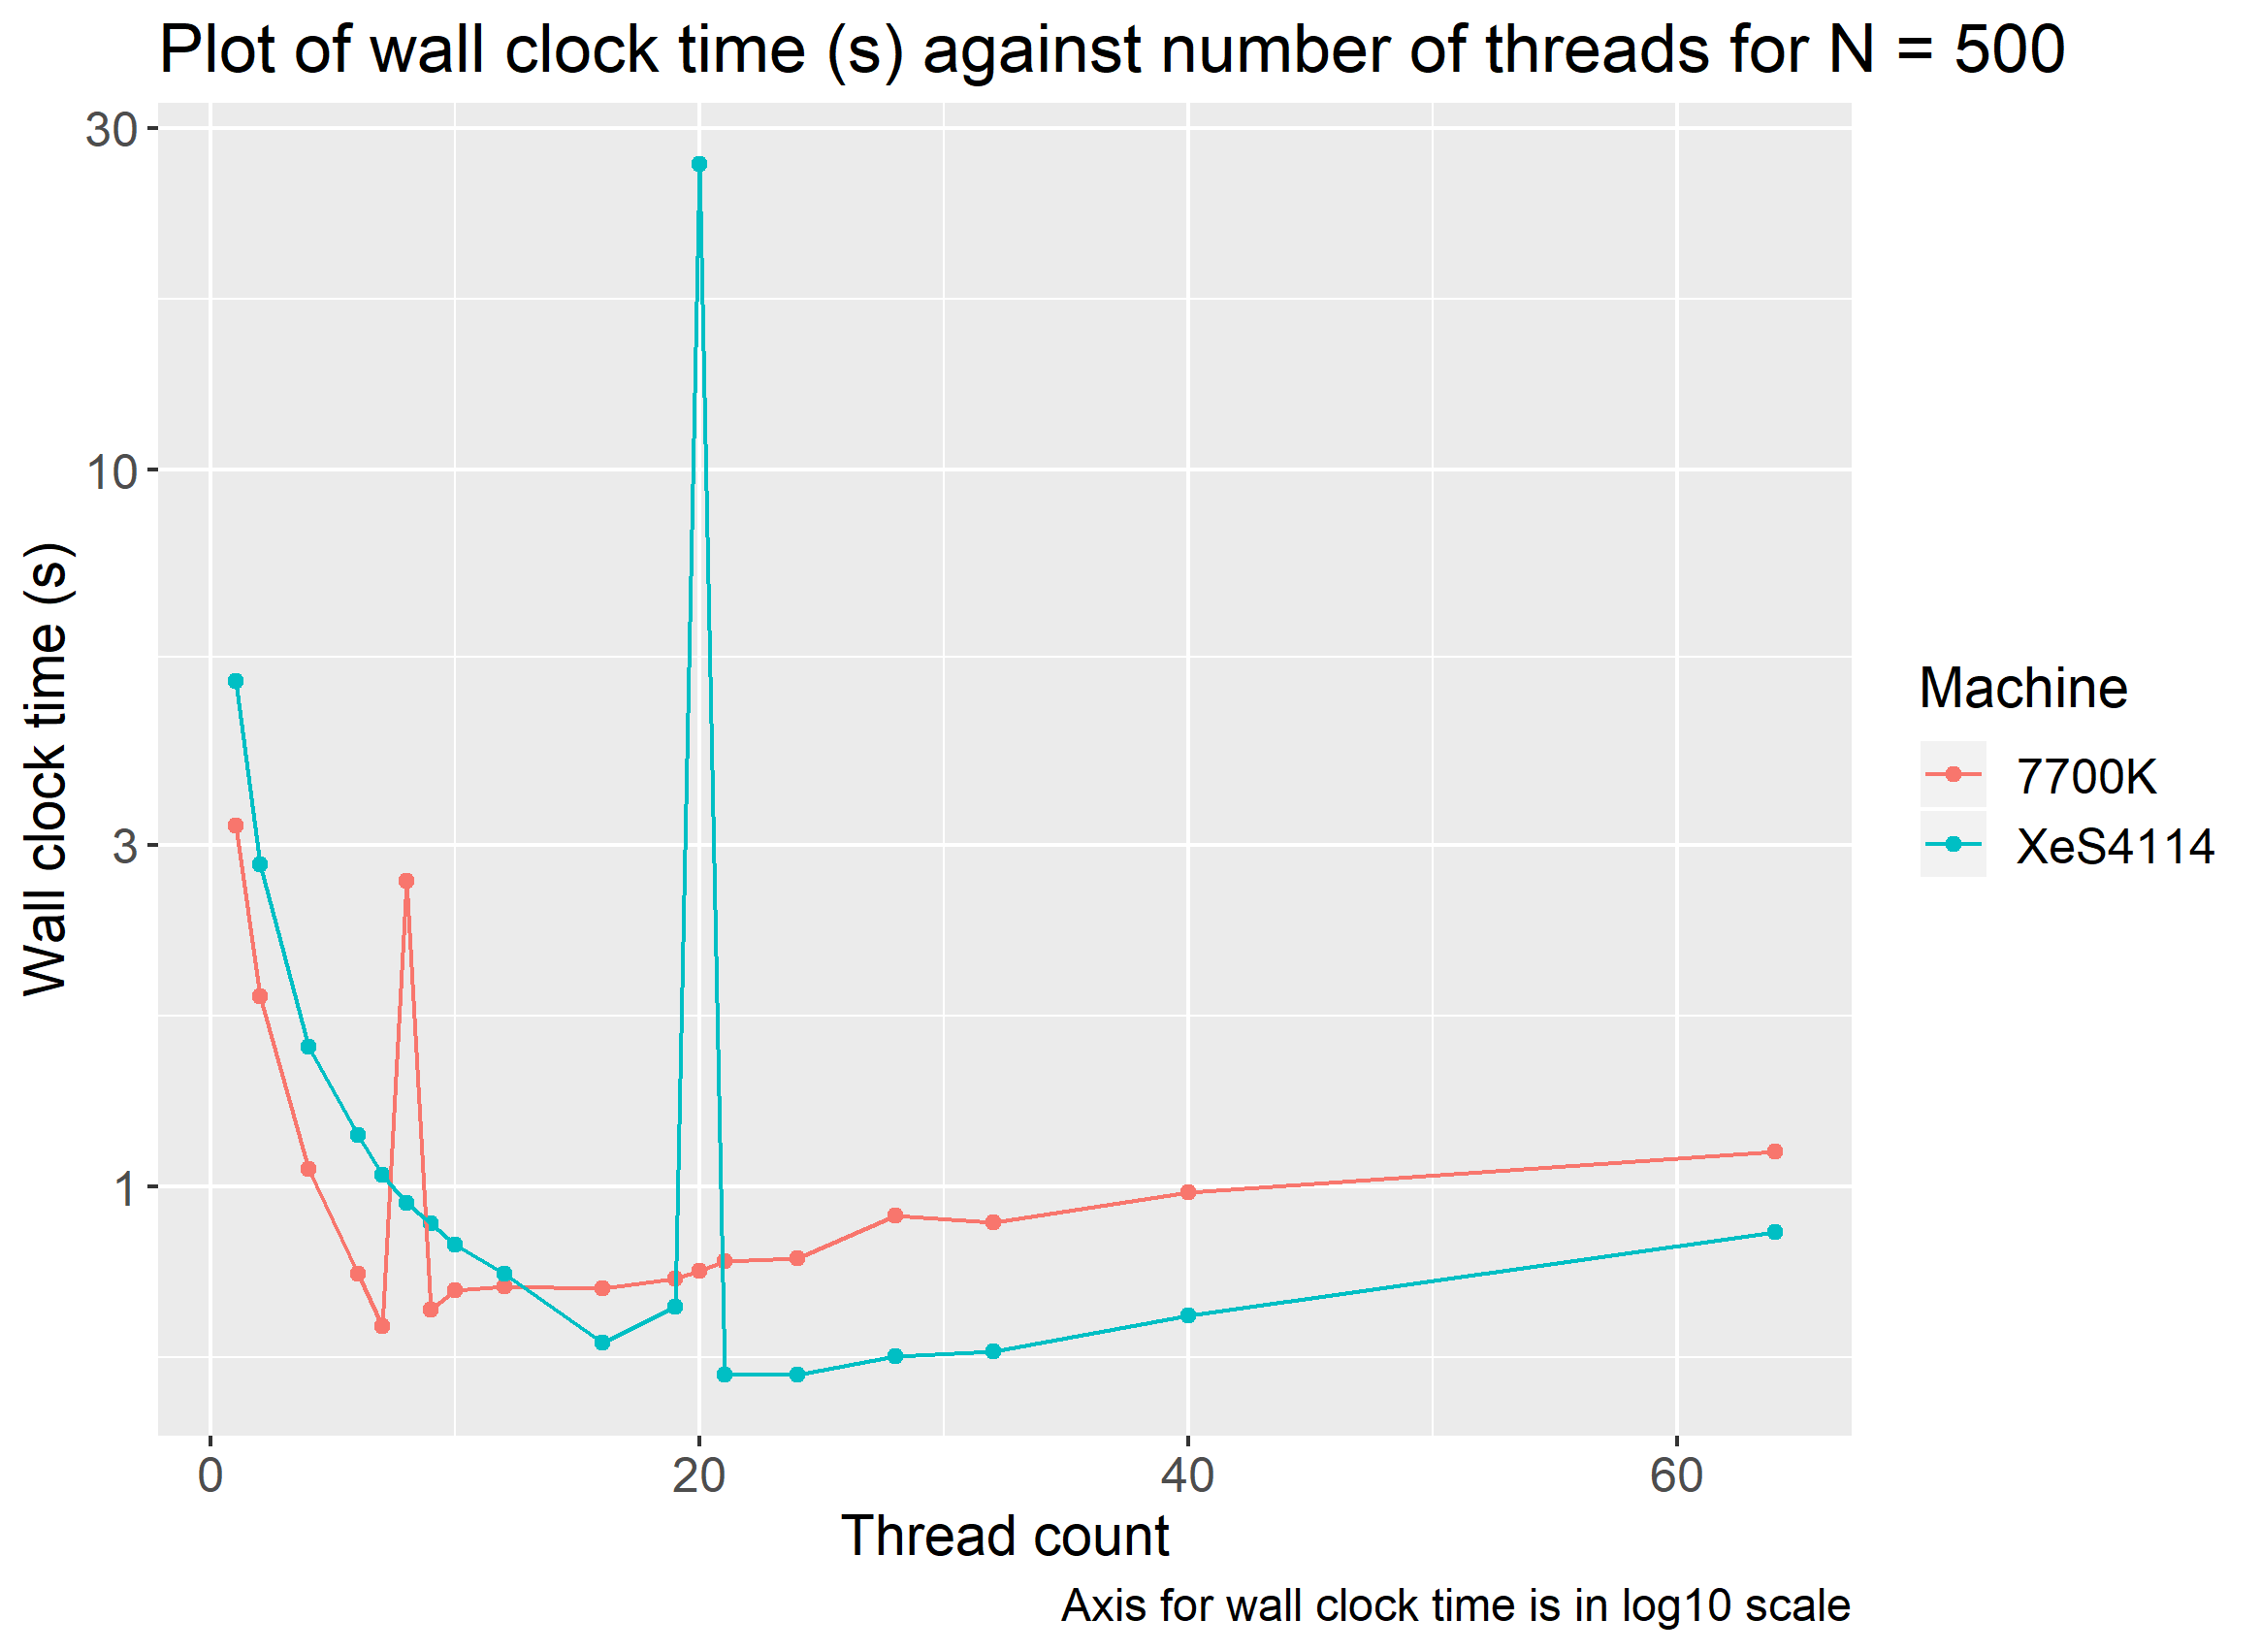
\includegraphics[width=0.75\textwidth]{par-500N-varyThreads}
    \caption{Plot of execution time against number of threads $T$ for $N = 500$}
    \label{fig:par-500N-varyThreads}
\end{figure}

\begin{figure}[H]
    \centering
    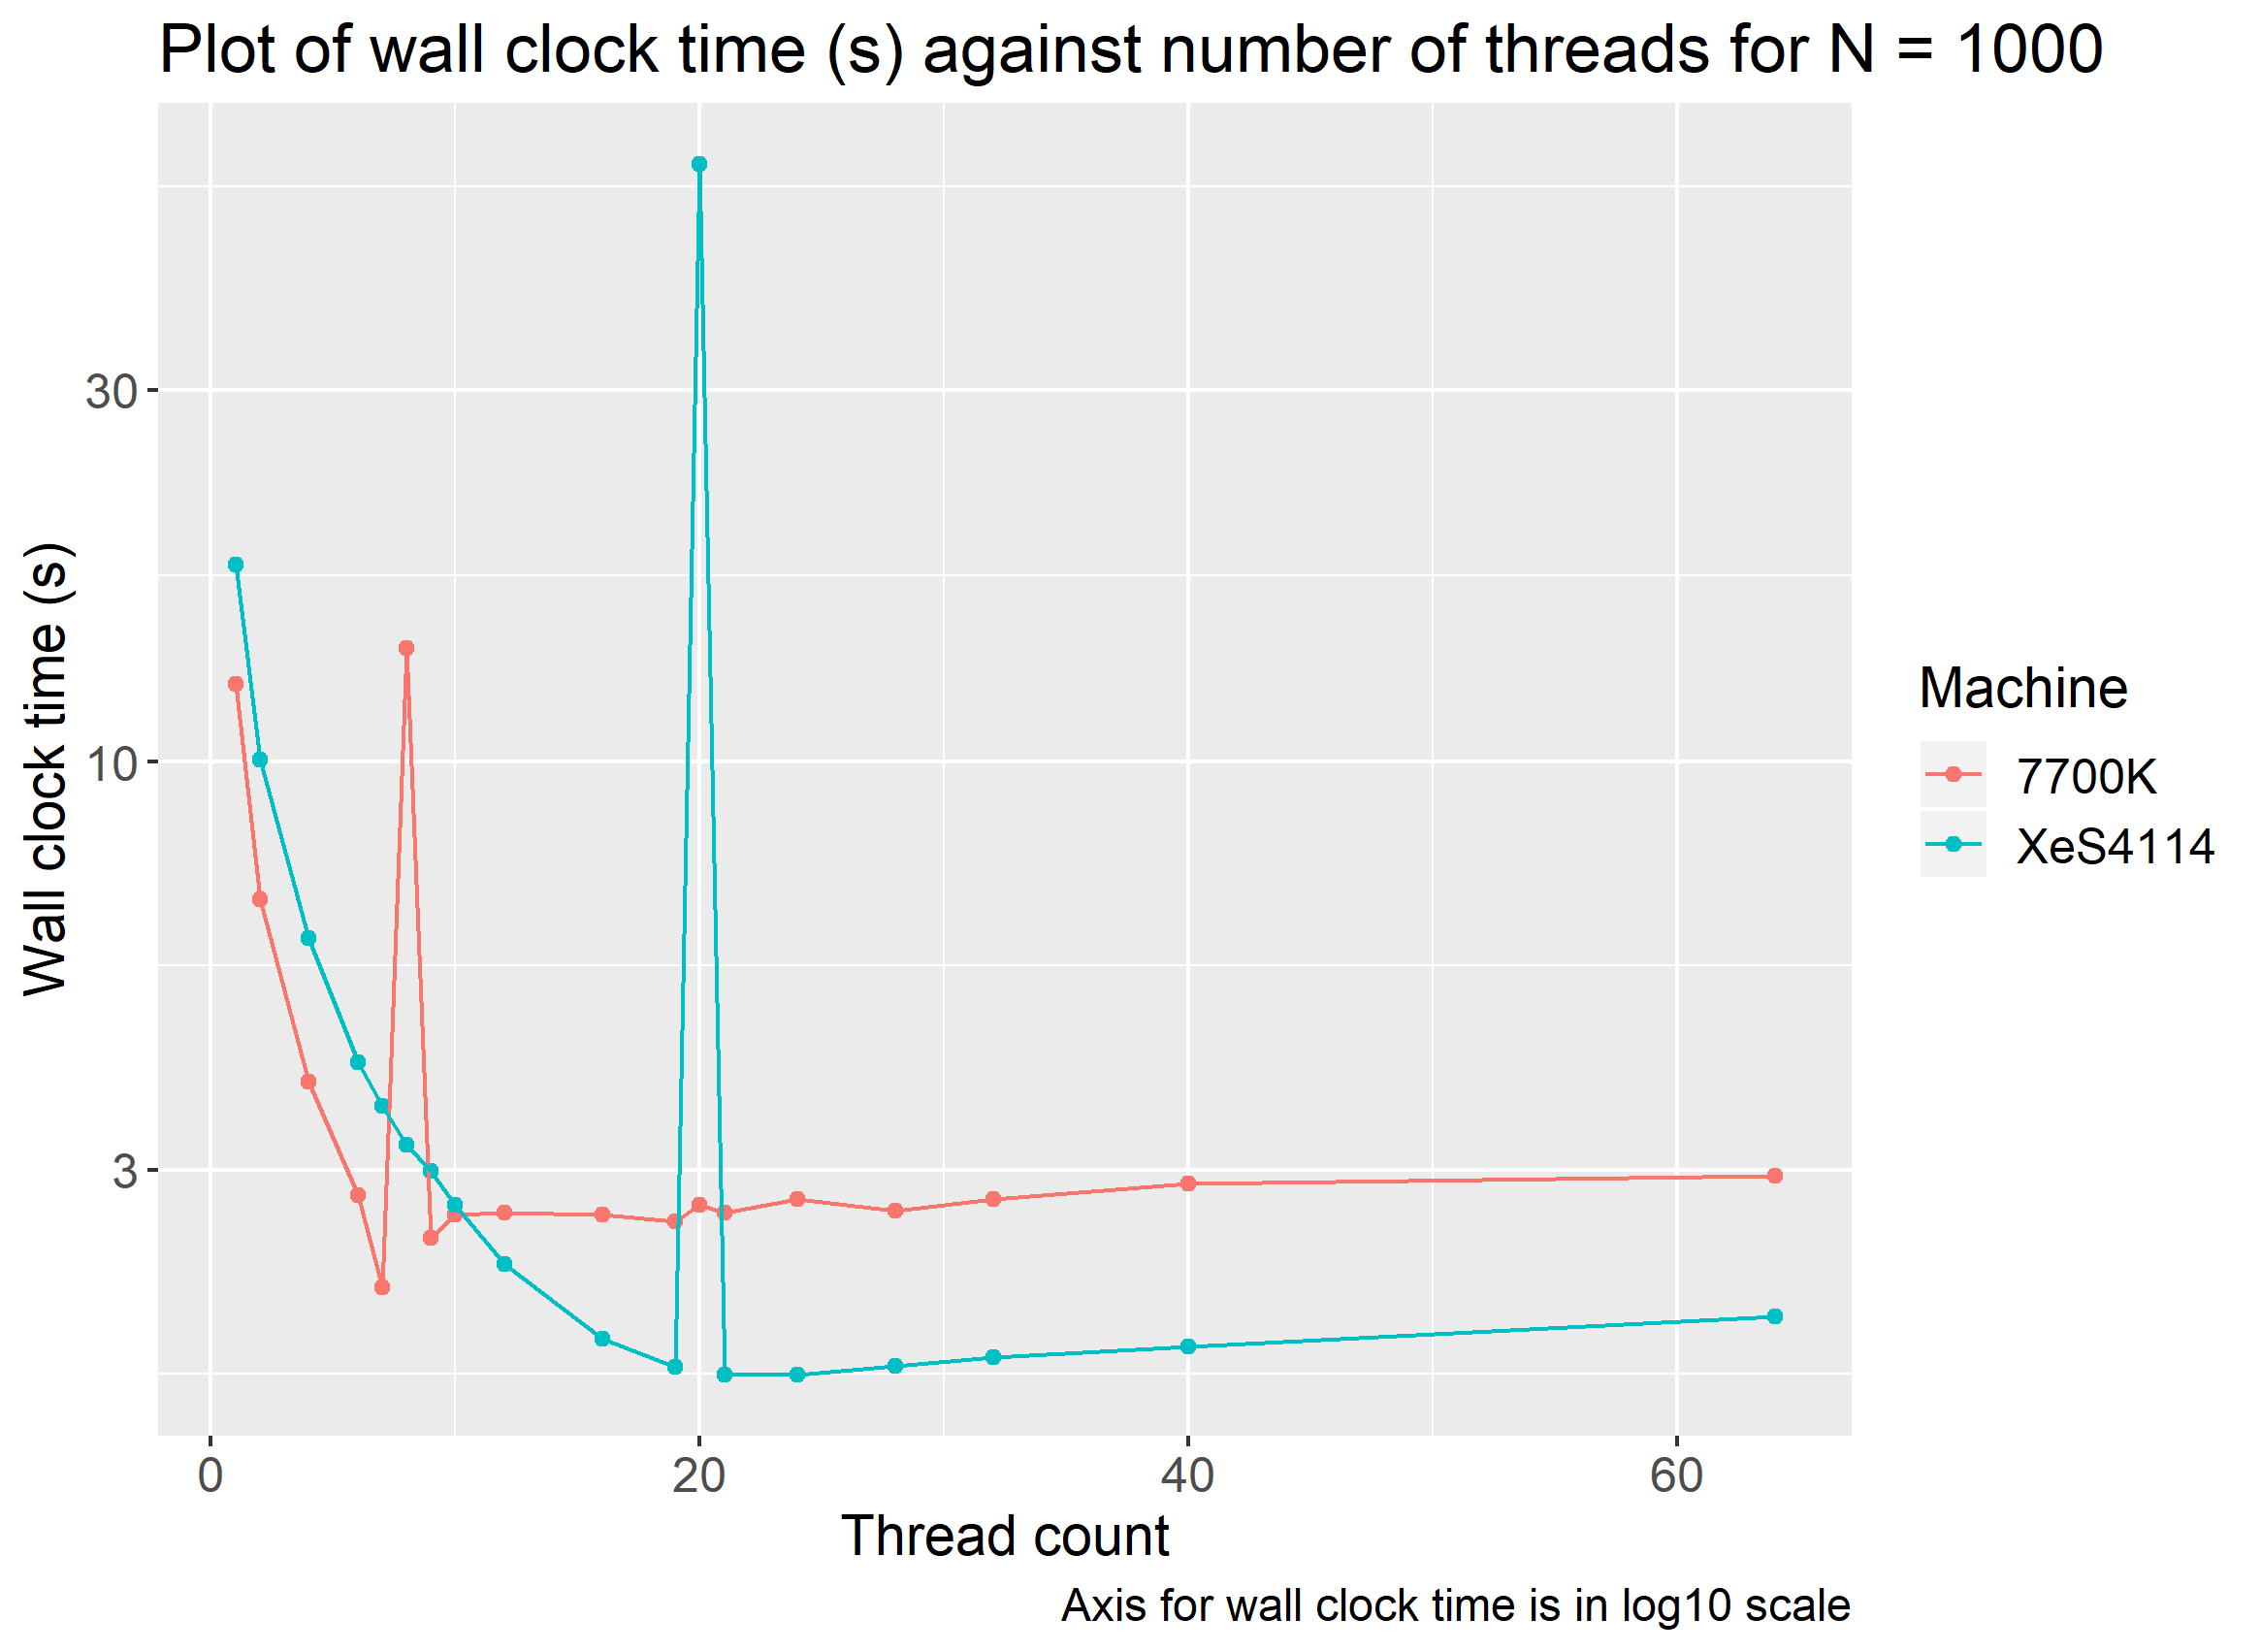
\includegraphics[width=0.75\textwidth]{par-1000N-varyThreads}
    \caption{Plot of execution time against number of threads $T$ for $N = 1000$}
    \label{fig:par-1000N-varyThreads}
\end{figure}

\begin{figure}[H]
    \centering
    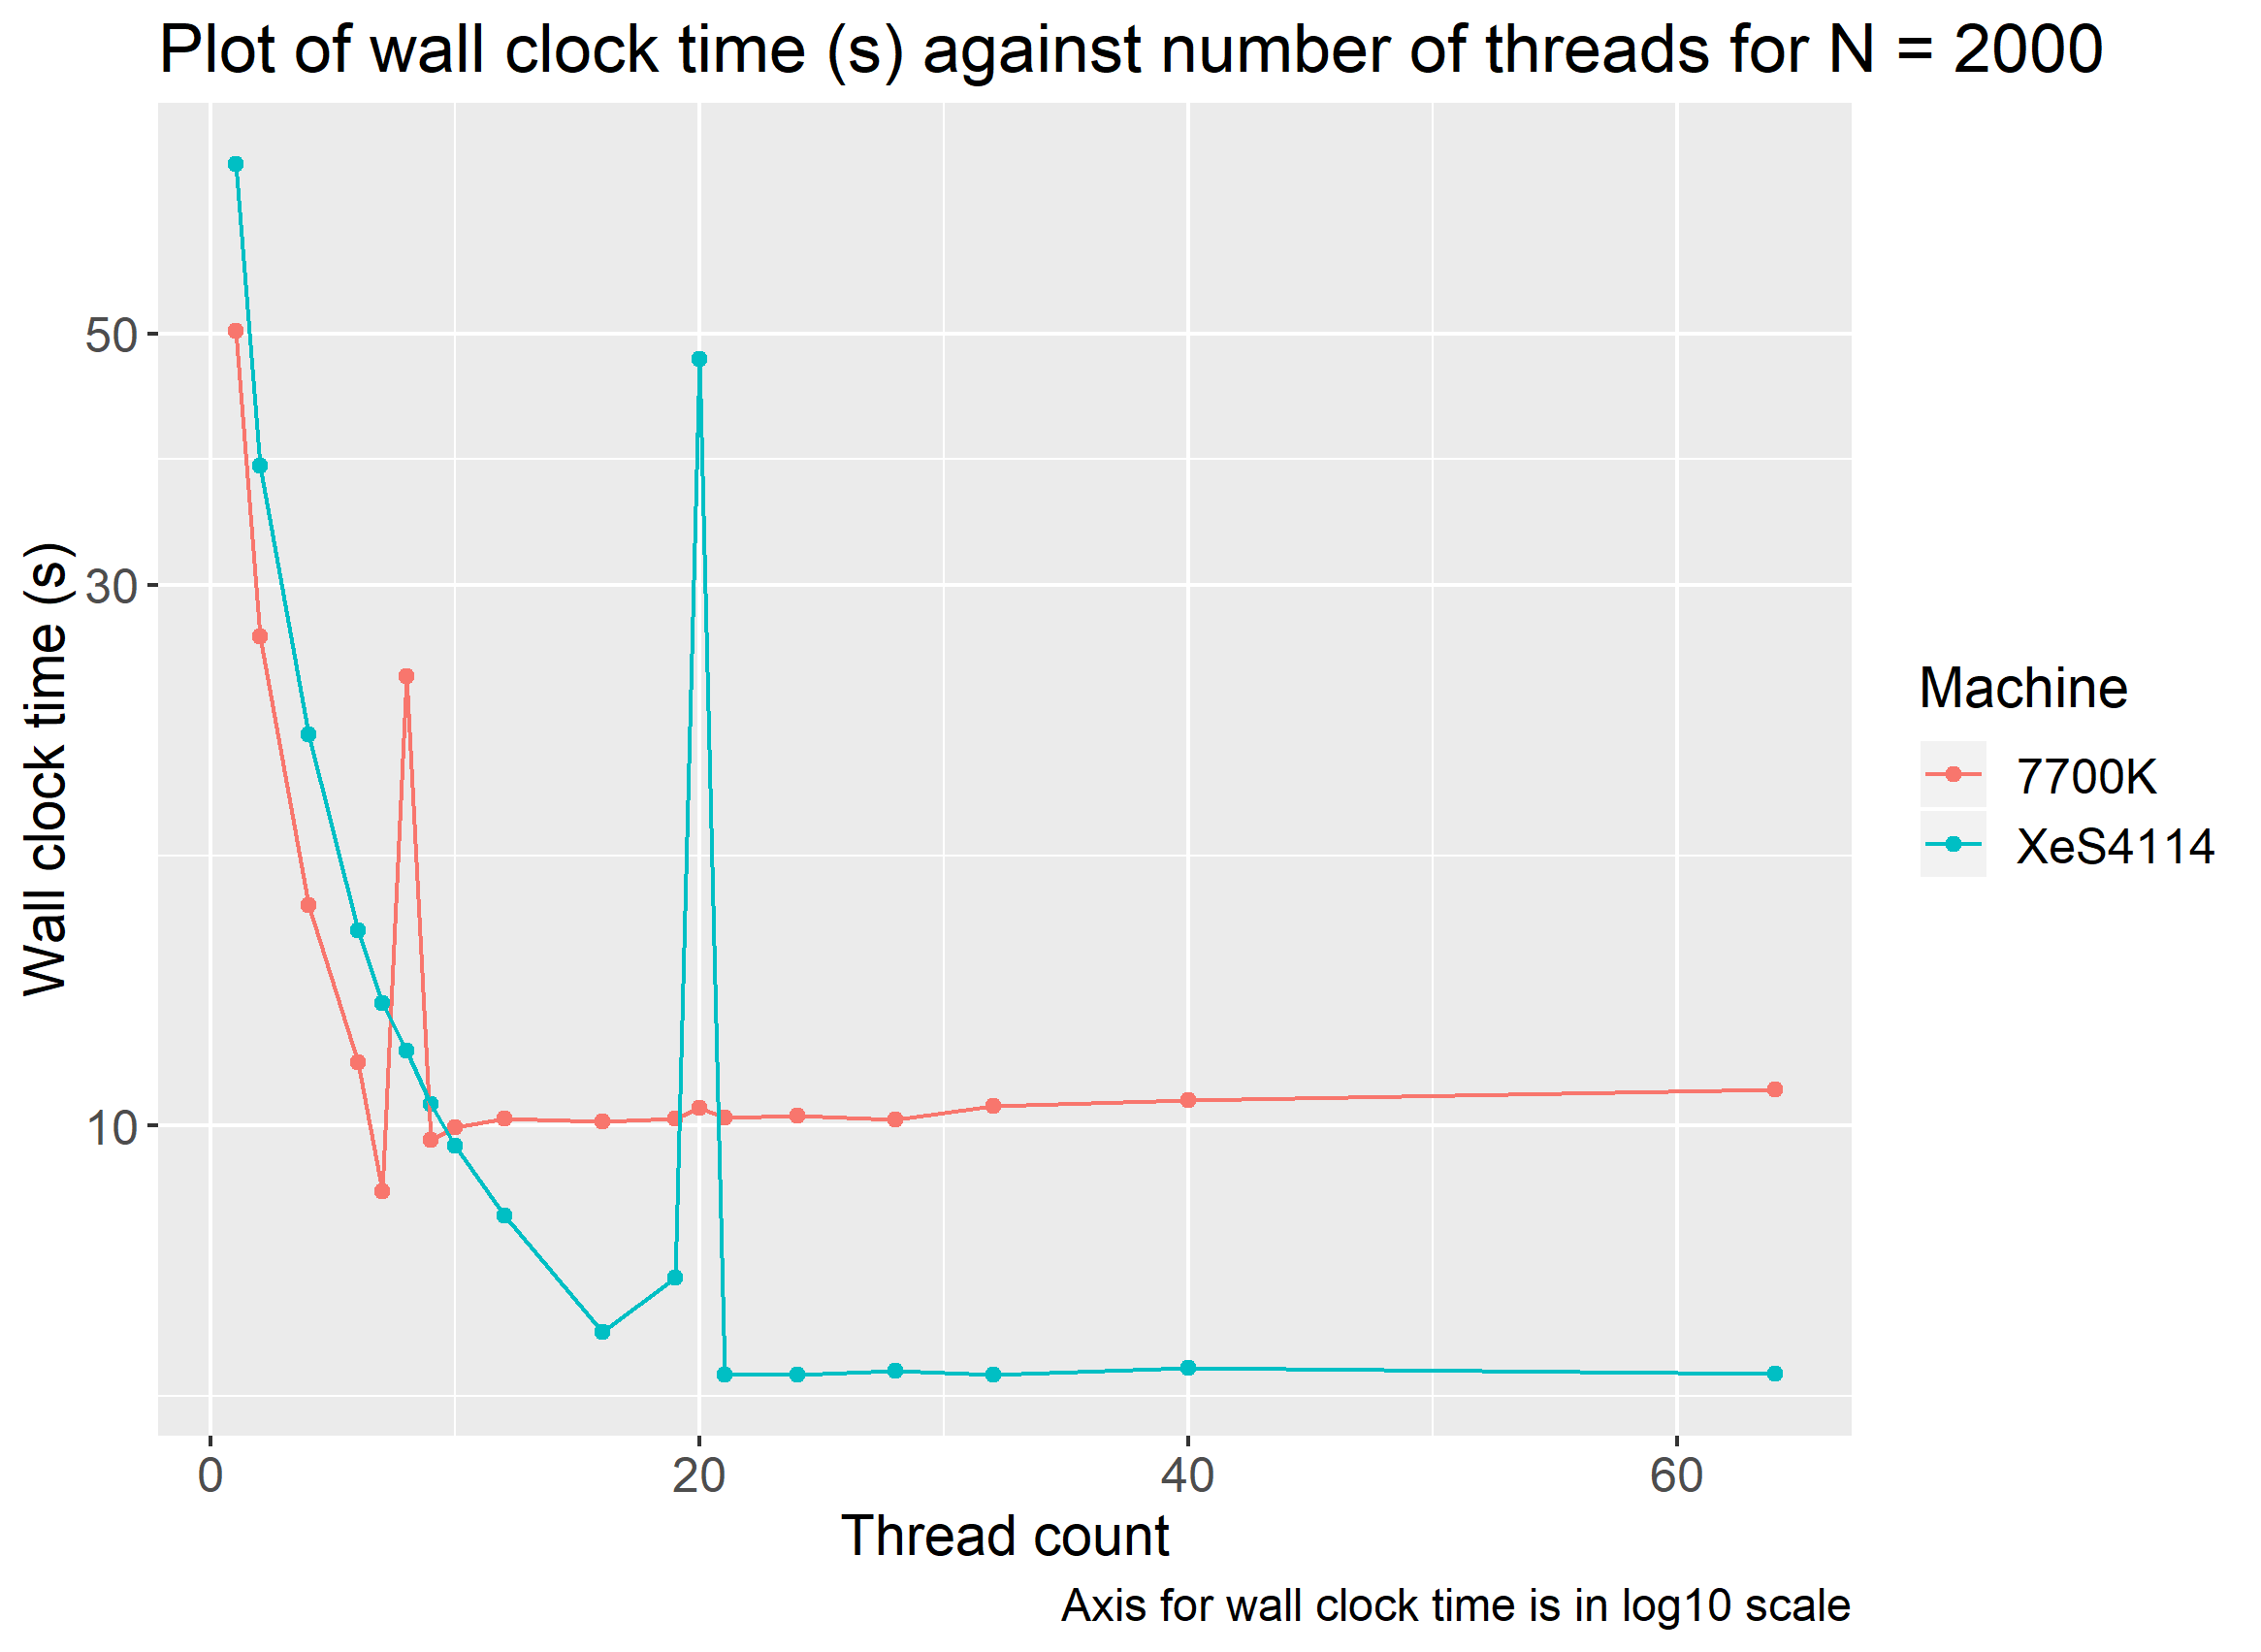
\includegraphics[width=0.75\textwidth]{par-2000N-varyThreads}
    \caption{Plot of execution time against number of threads $T$ for $N = 2000$}
    \label{fig:par-2000N-varyThreads}
\end{figure}

\subsection{Speedup between sequential and parallel implementation}

\begin{figure}[H]
    \centering
    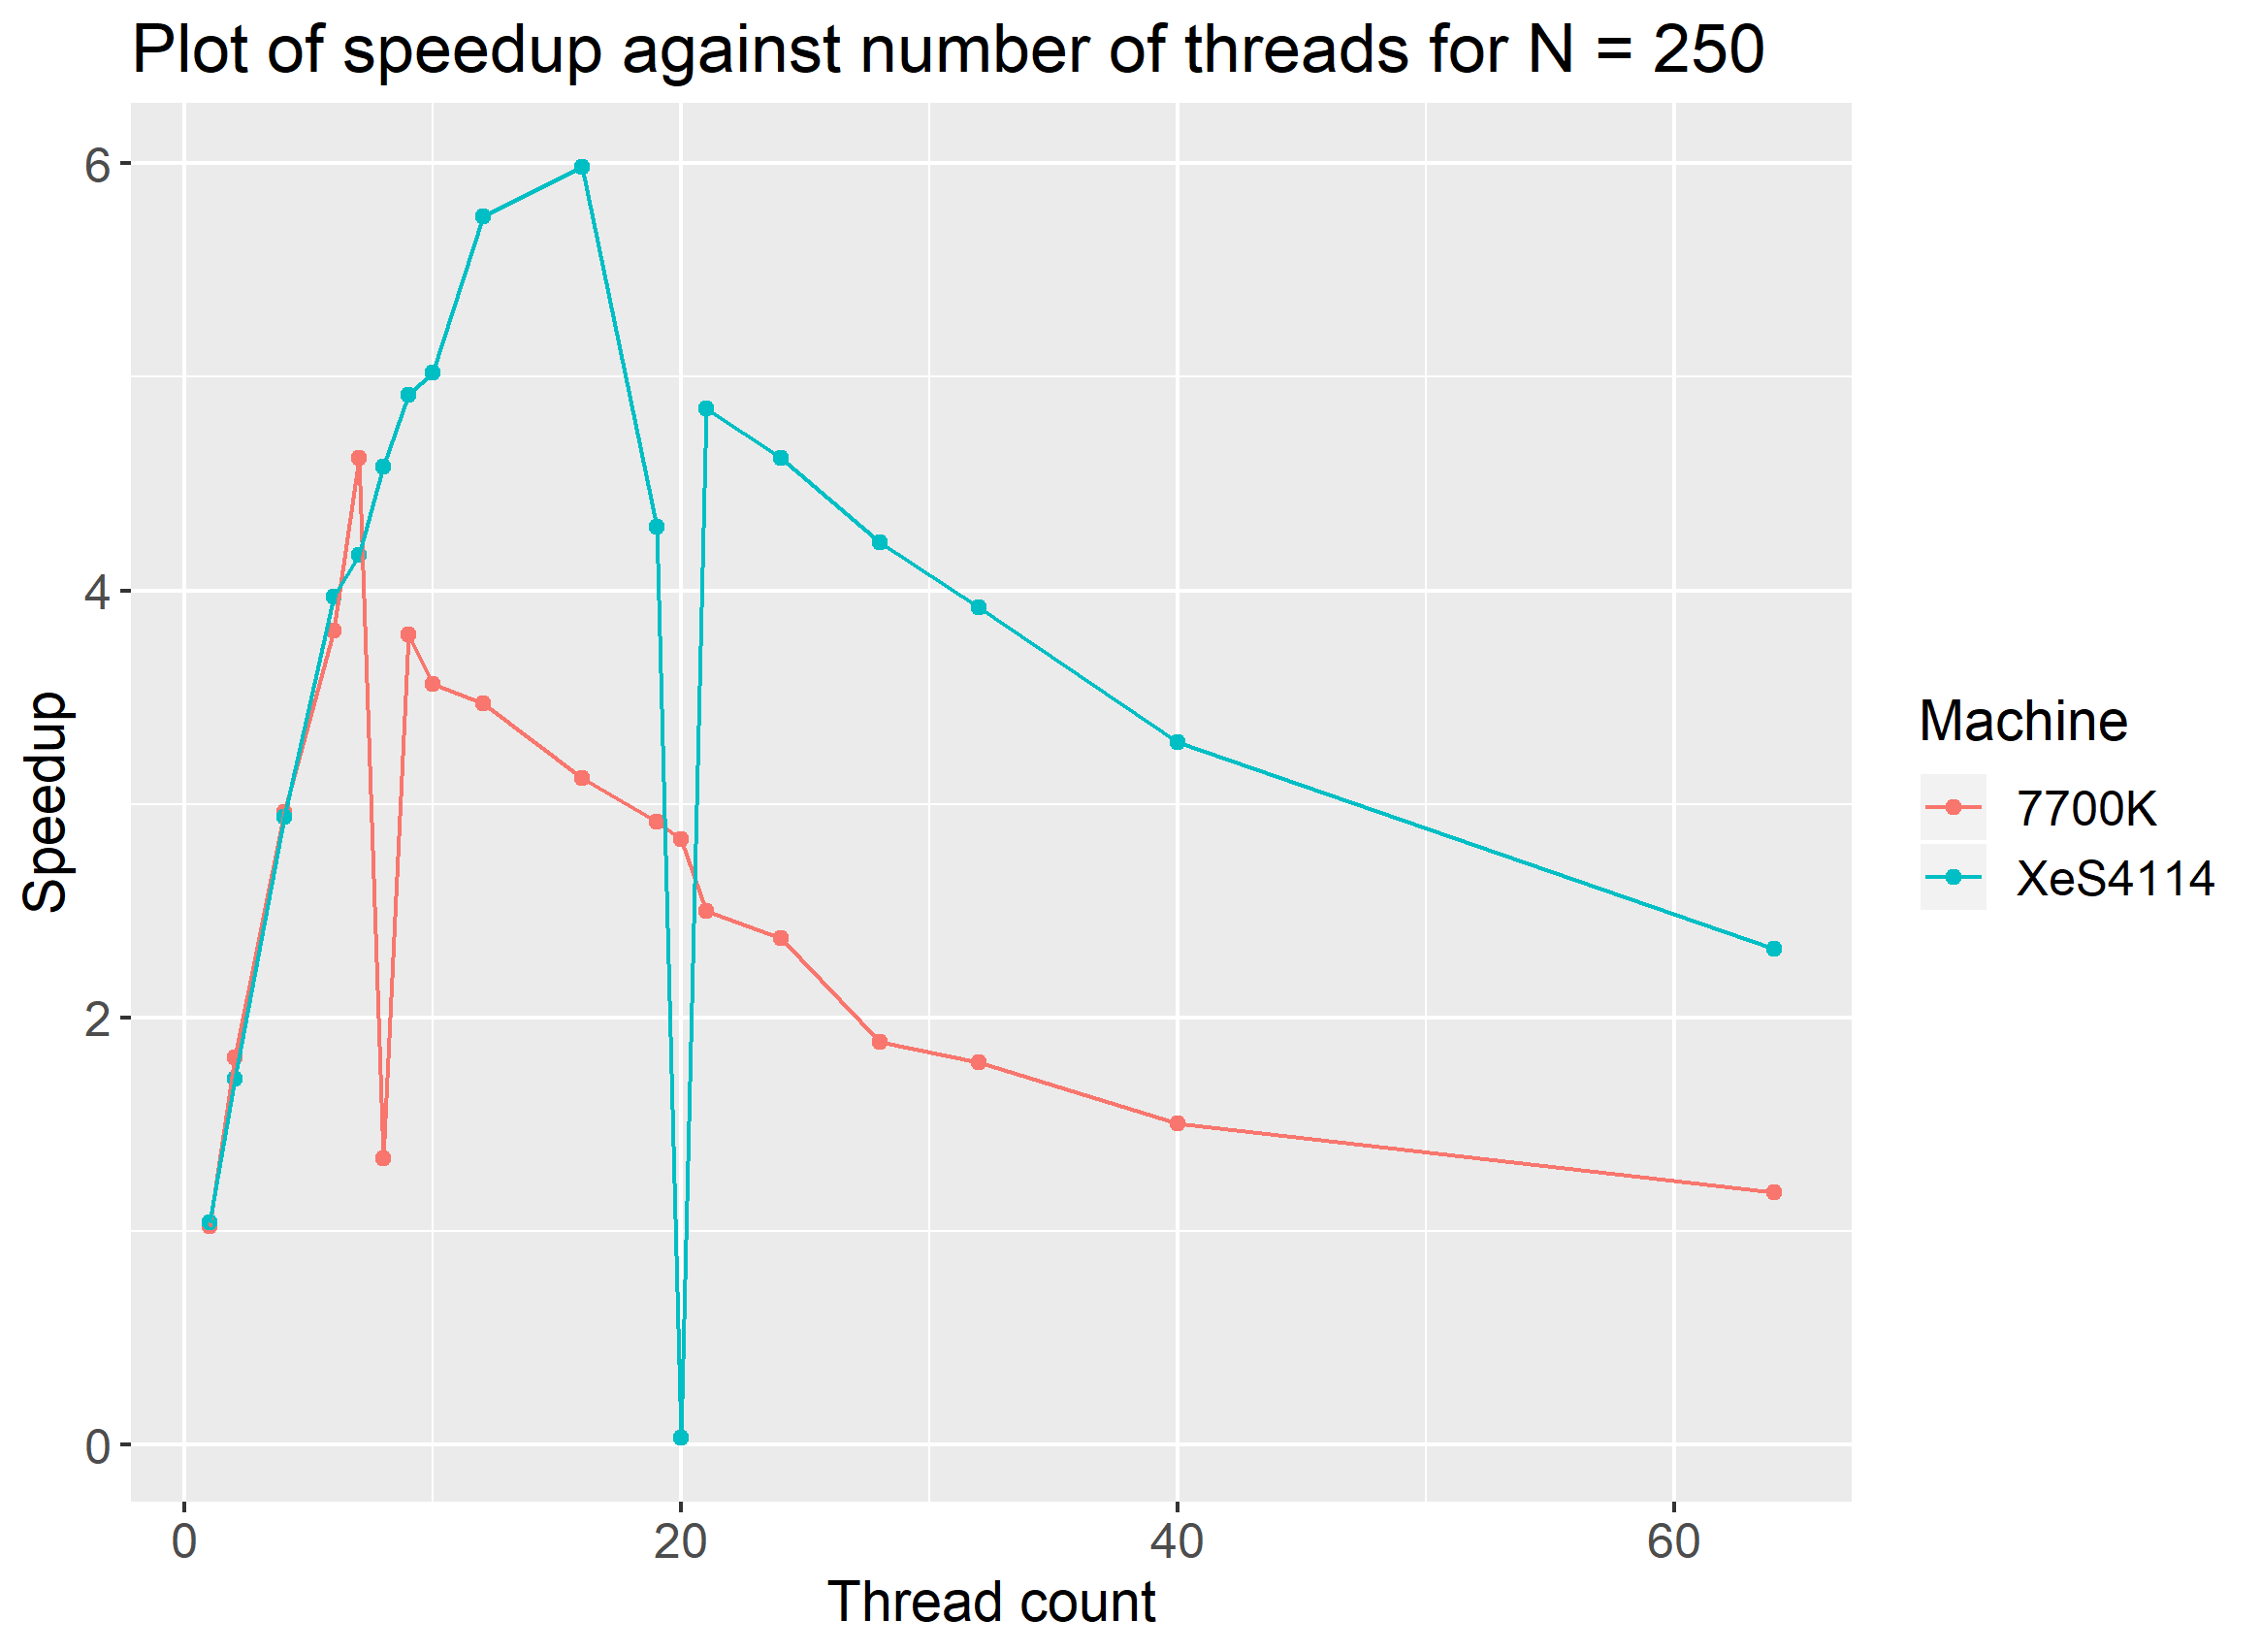
\includegraphics[width=0.75\textwidth]{par-250N-speedup}
    \caption{Plot of speedup against number of threads $T$ for $N = 250$}
    \label{fig:par-250N-speedup}
\end{figure}

\begin{figure}[H]
    \centering
    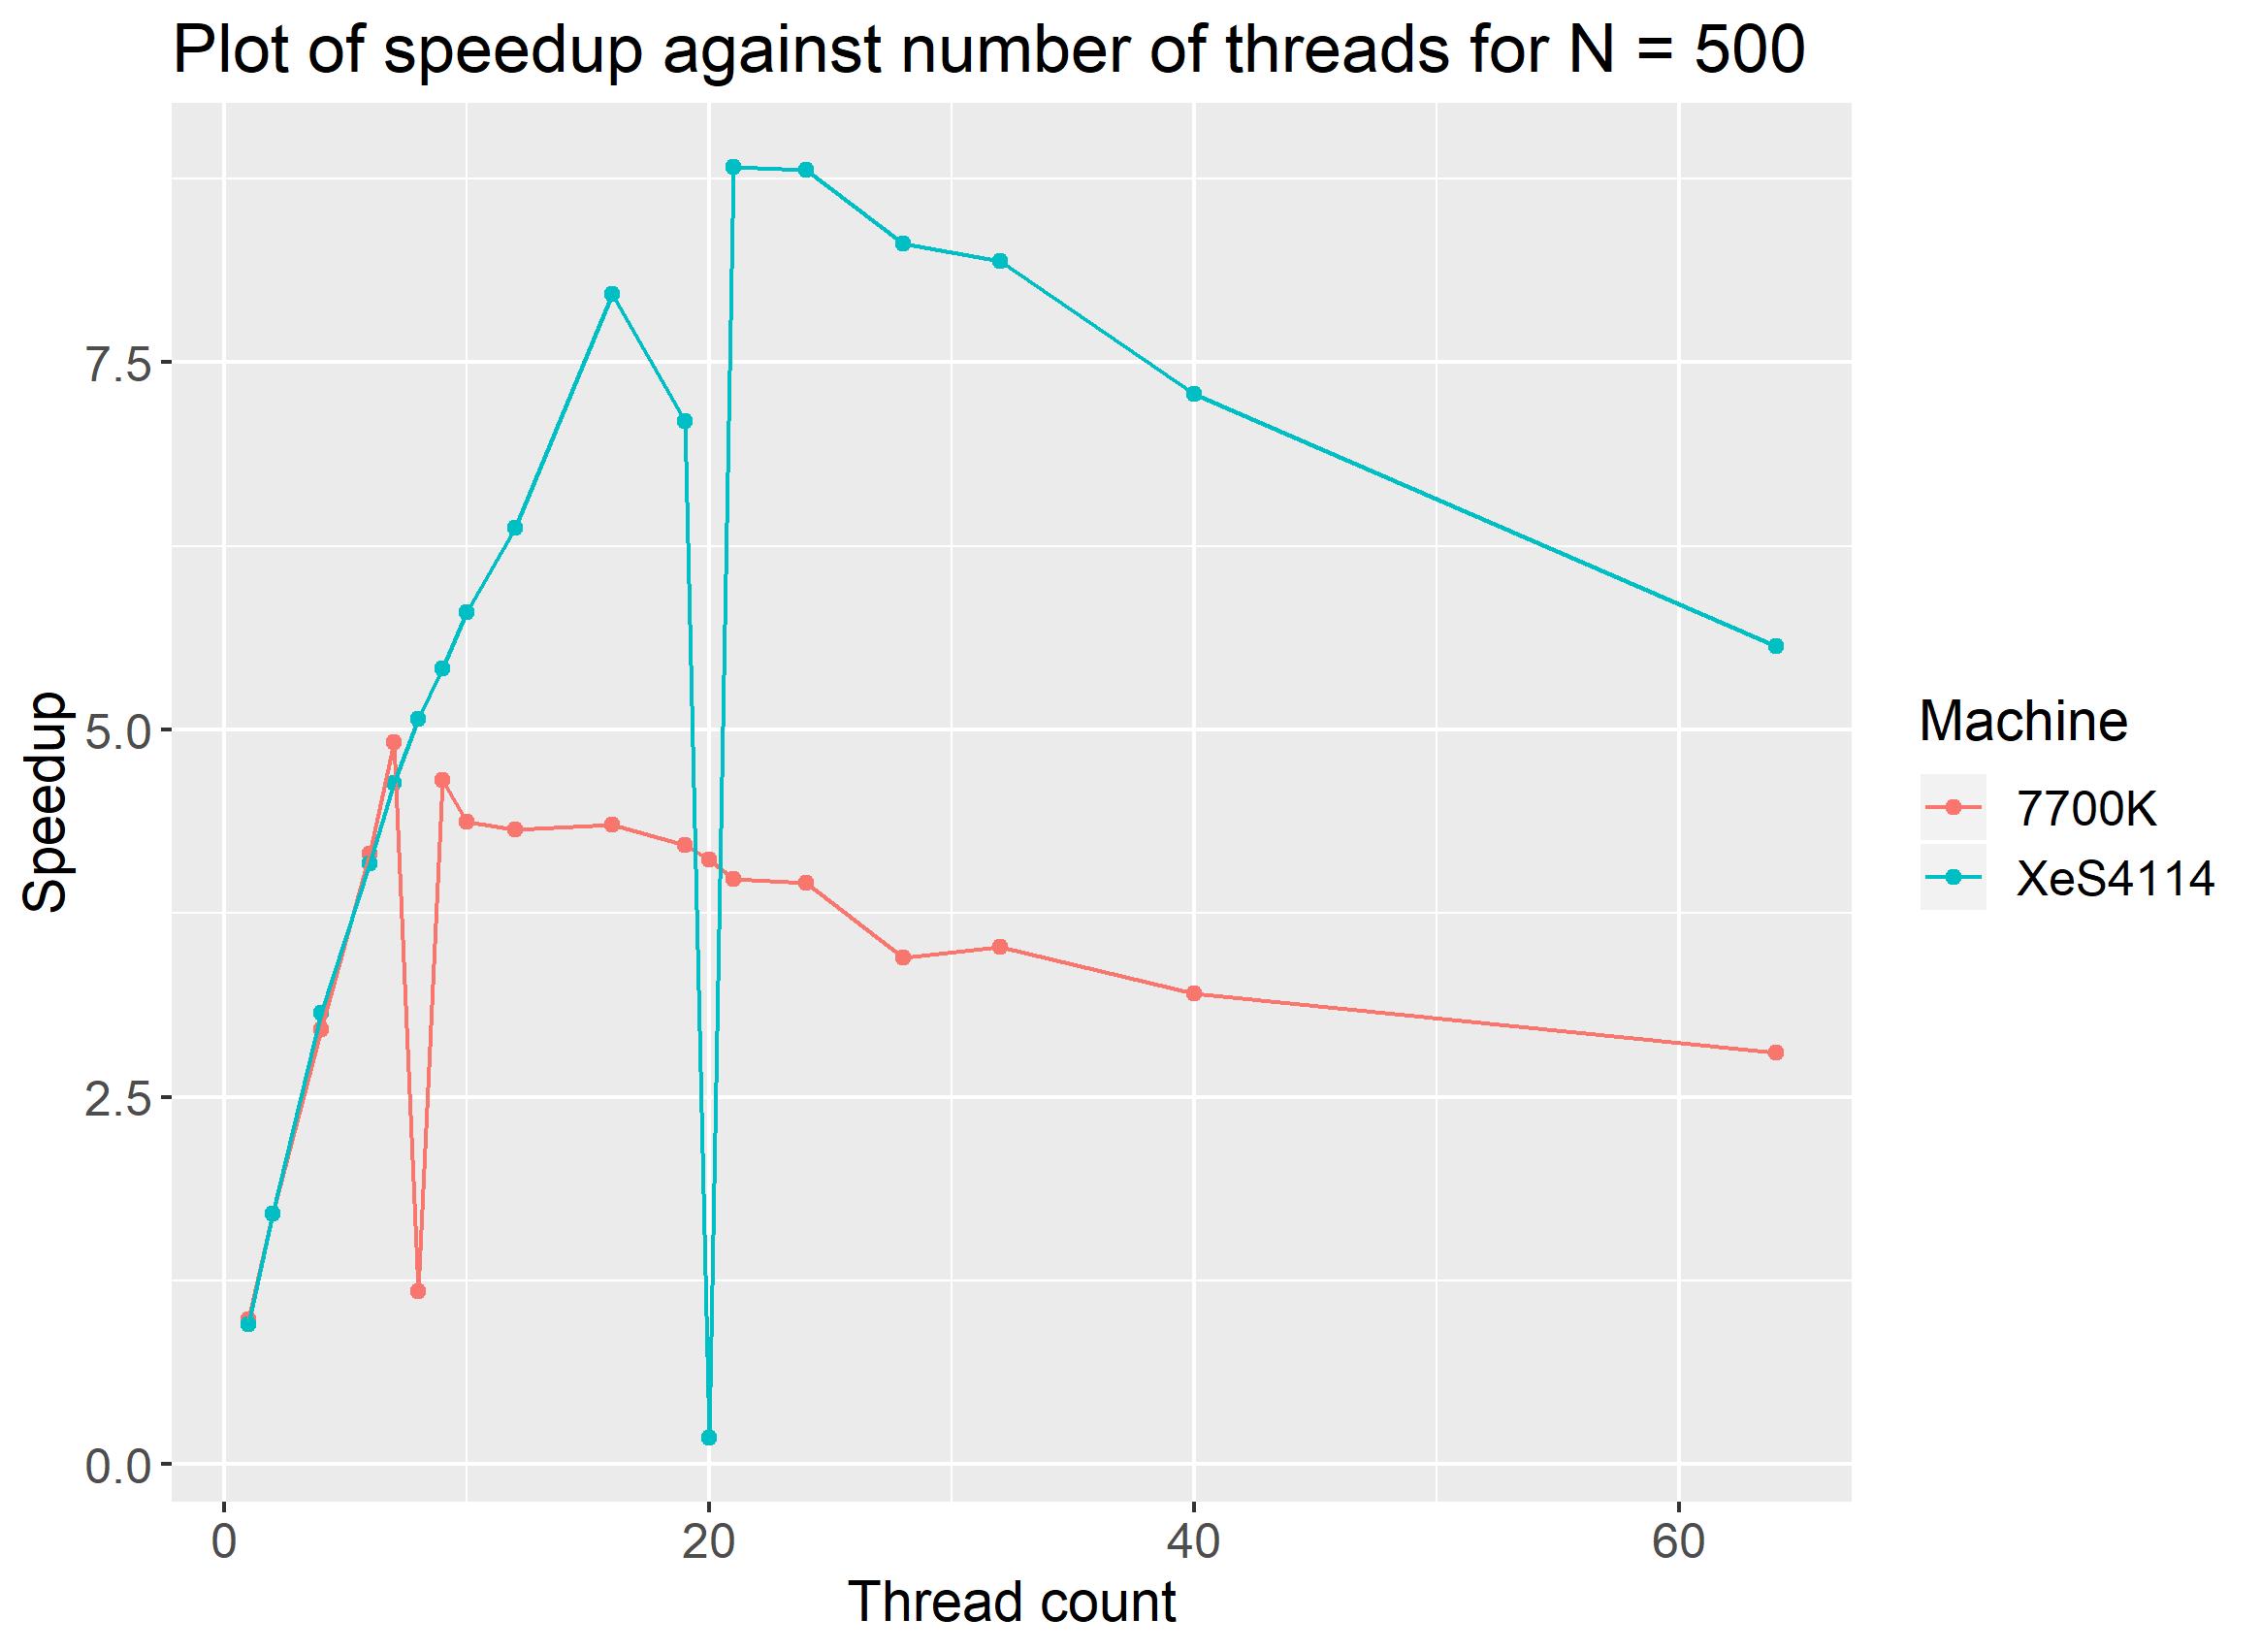
\includegraphics[width=0.75\textwidth]{par-500N-speedup}
    \caption{Plot of speedup against number of threads $T$ for $N = 500$}
    \label{fig:par-500N-speedup}
\end{figure}

\begin{figure}[H]
    \centering
    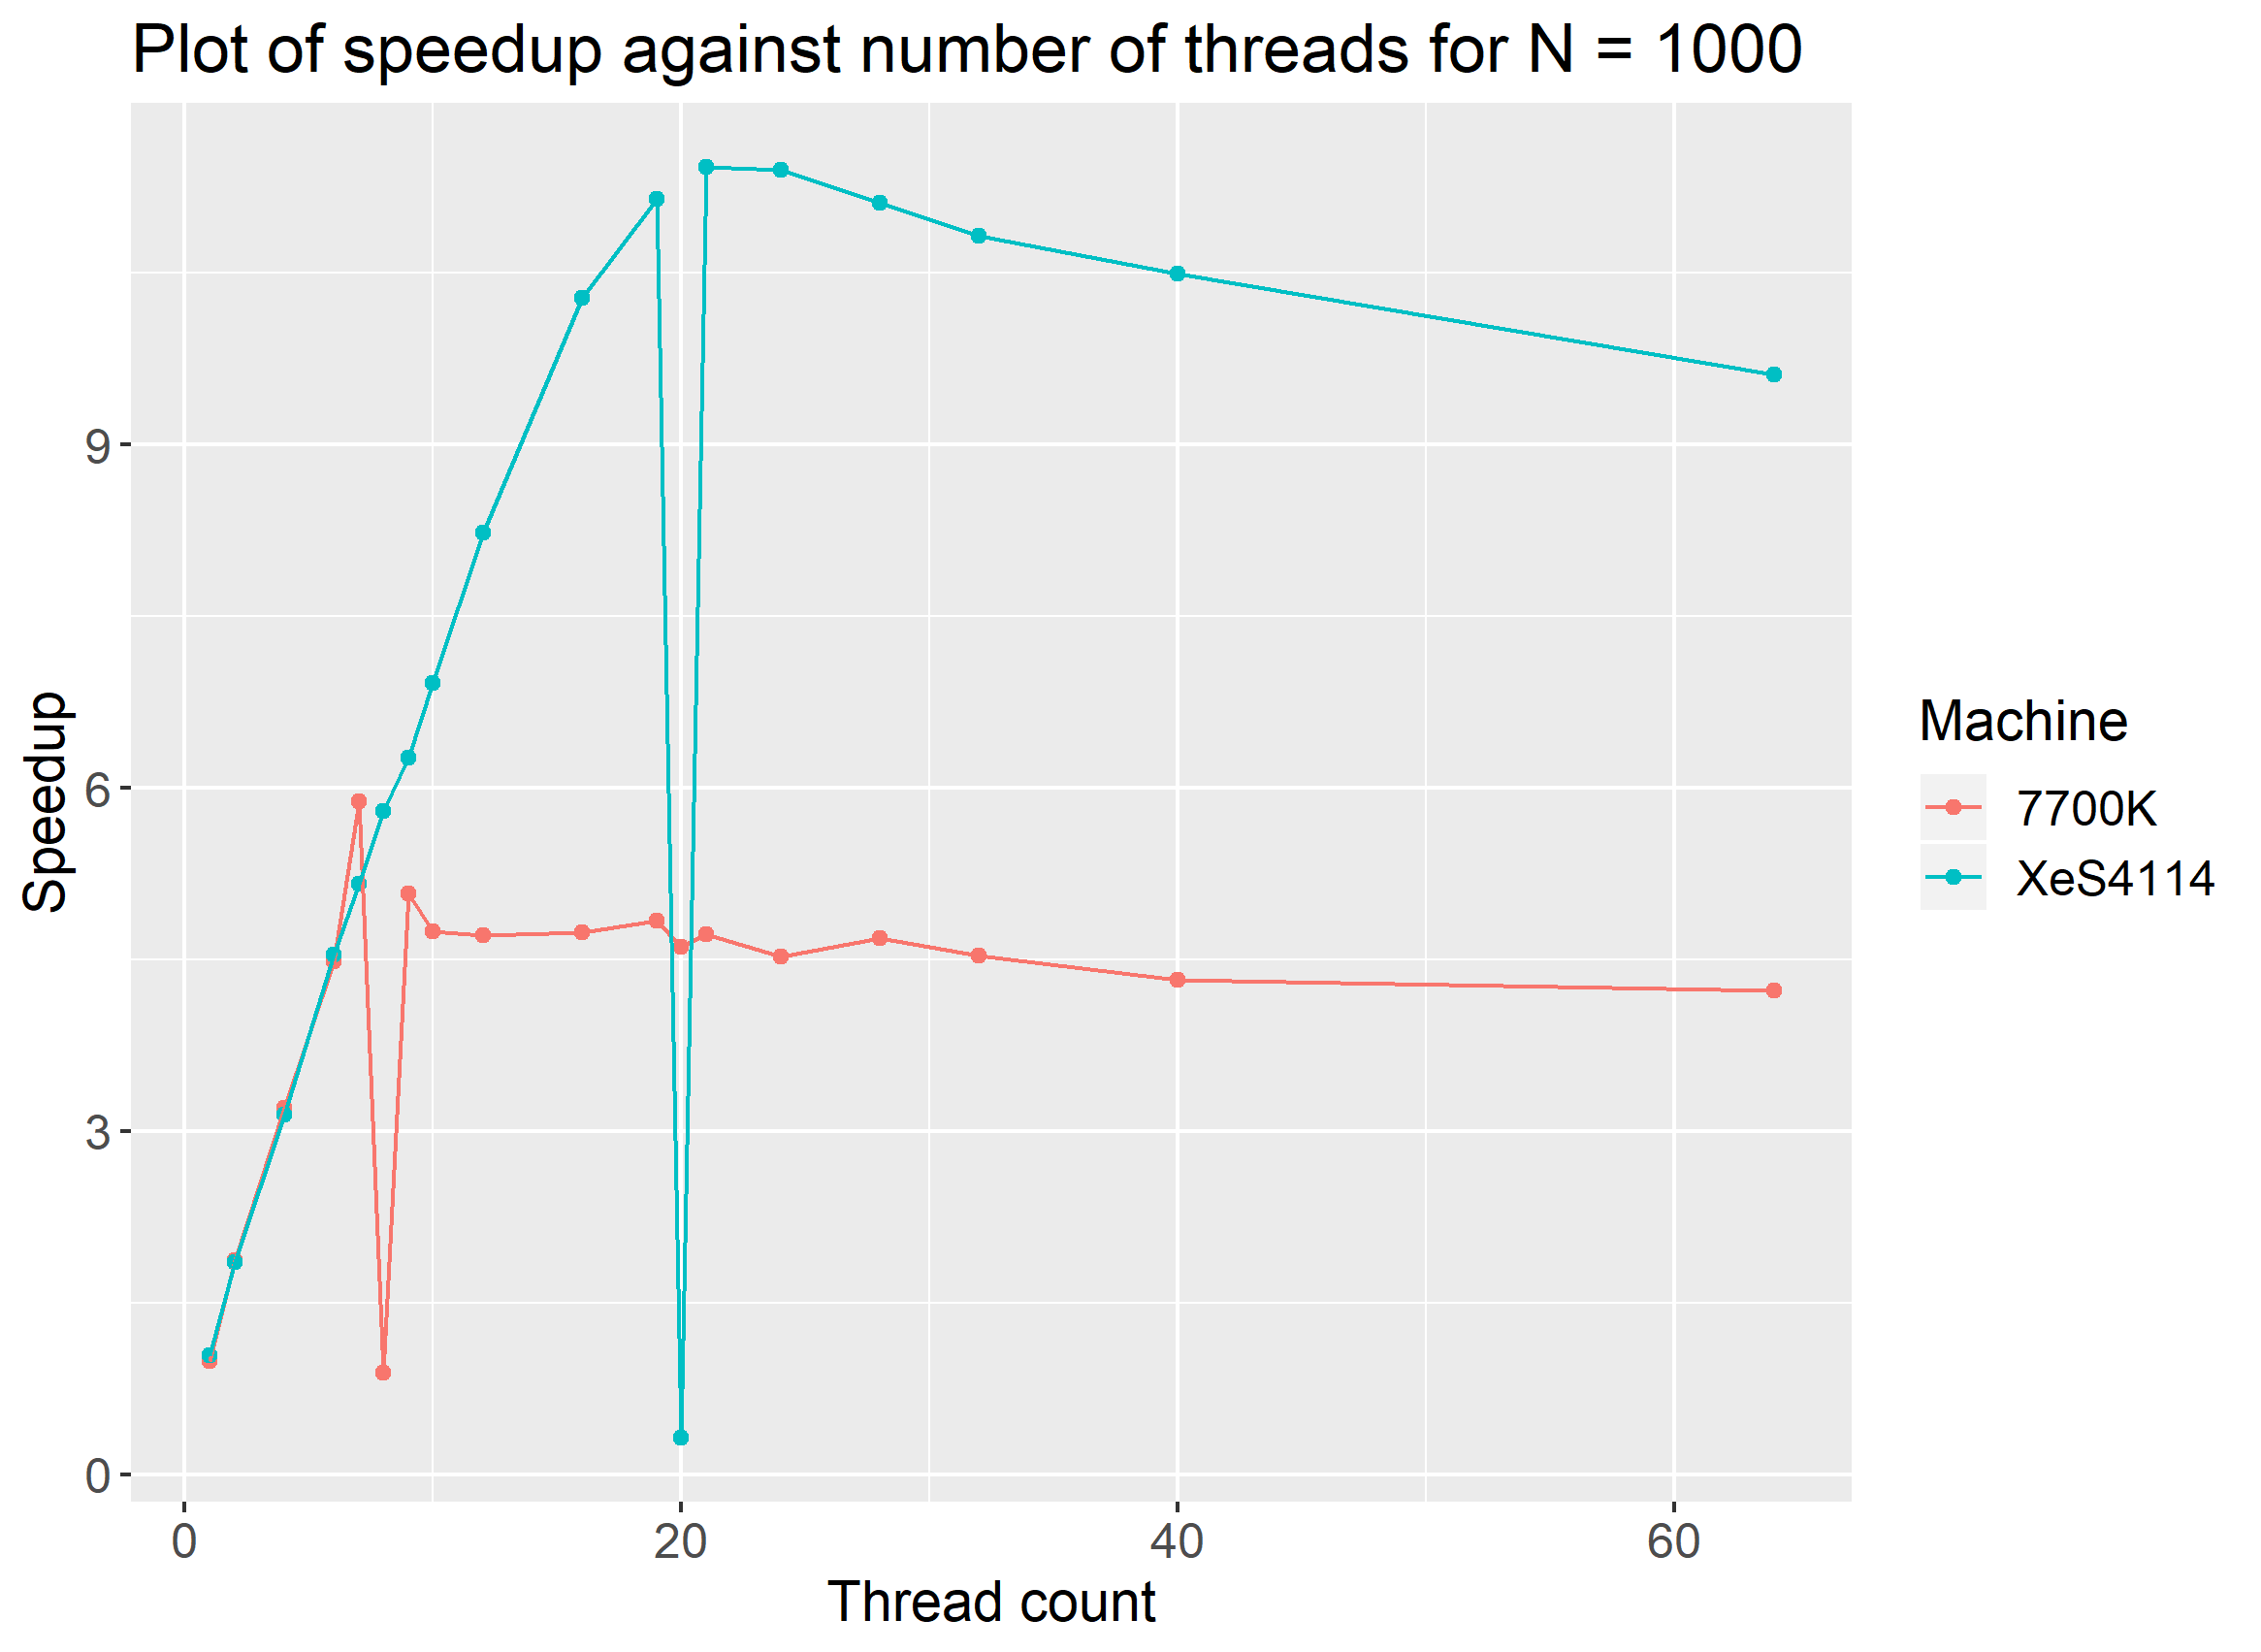
\includegraphics[width=0.75\textwidth]{par-1000N-speedup}
    \caption{Plot of speedup against number of threads $T$ for $N = 1000$}
    \label{fig:par-1000N-speedup}
\end{figure}

\begin{figure}[H]
    \centering
    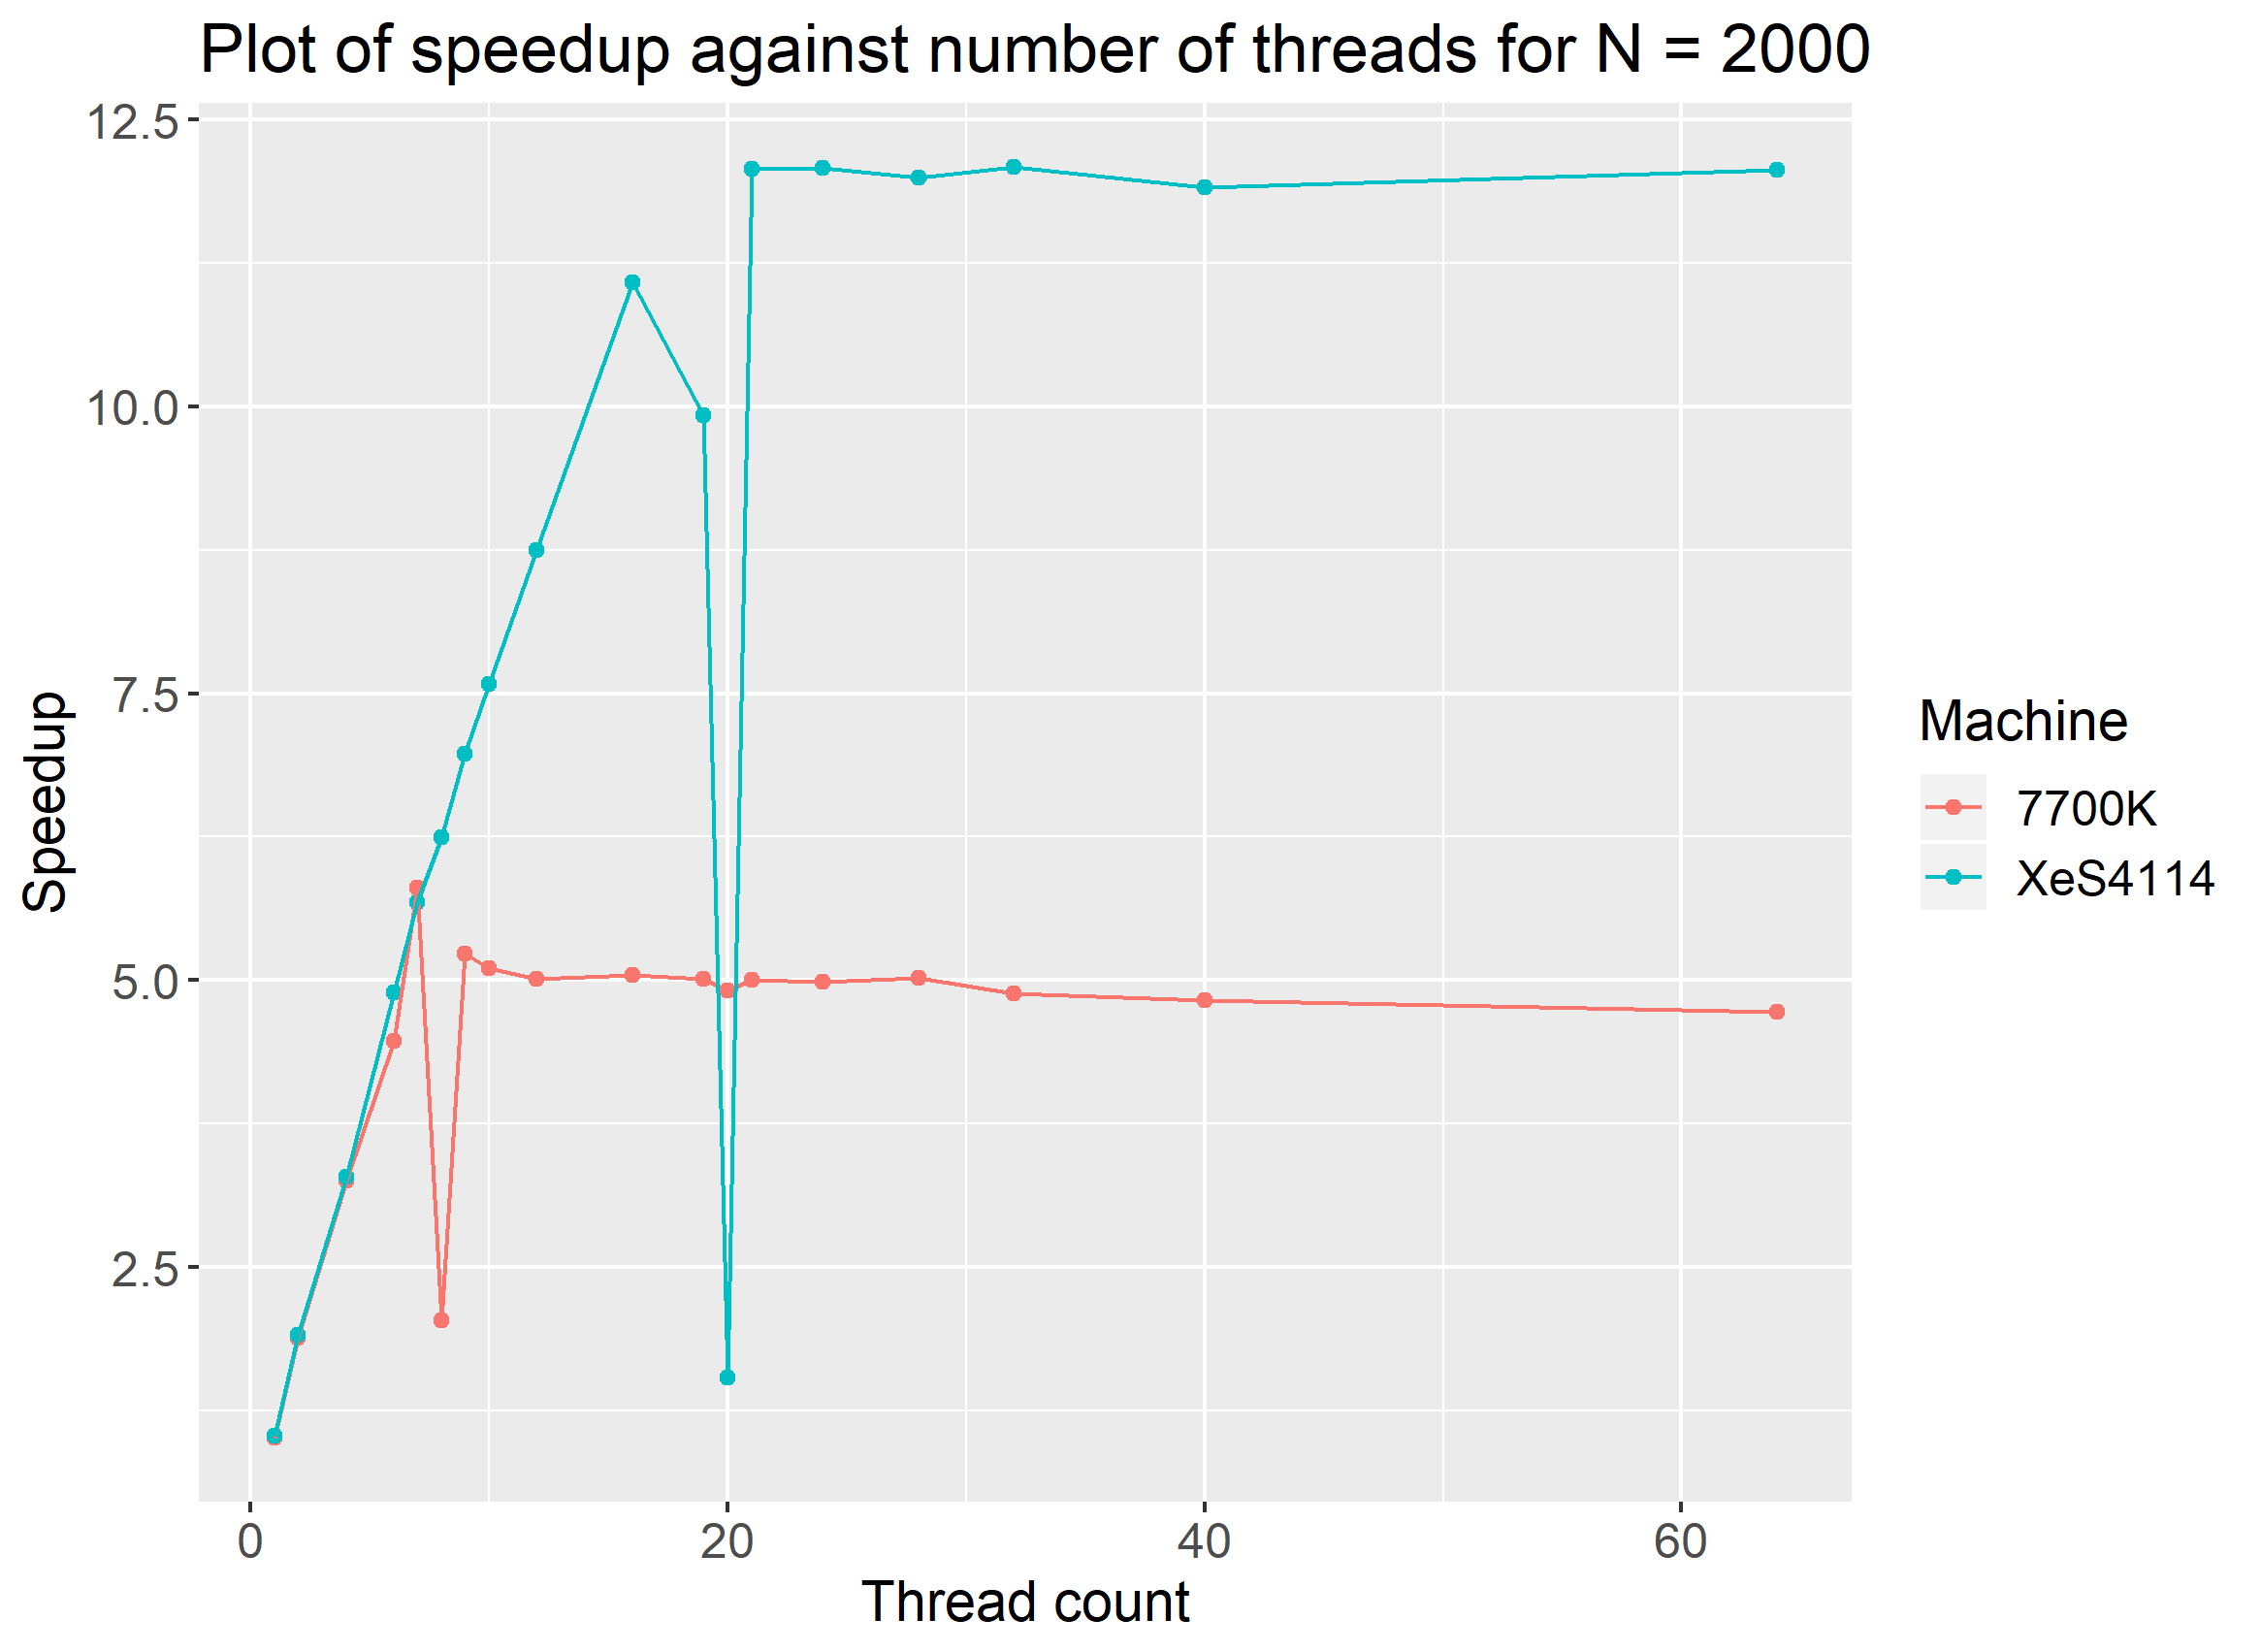
\includegraphics[width=0.75\textwidth]{par-2000N-speedup}
    \caption{Plot of speedup against number of threads $T$ for $N = 2000$}
    \label{fig:par-2000N-speedup}
\end{figure}

\begin{figure}[H]
    \centering
    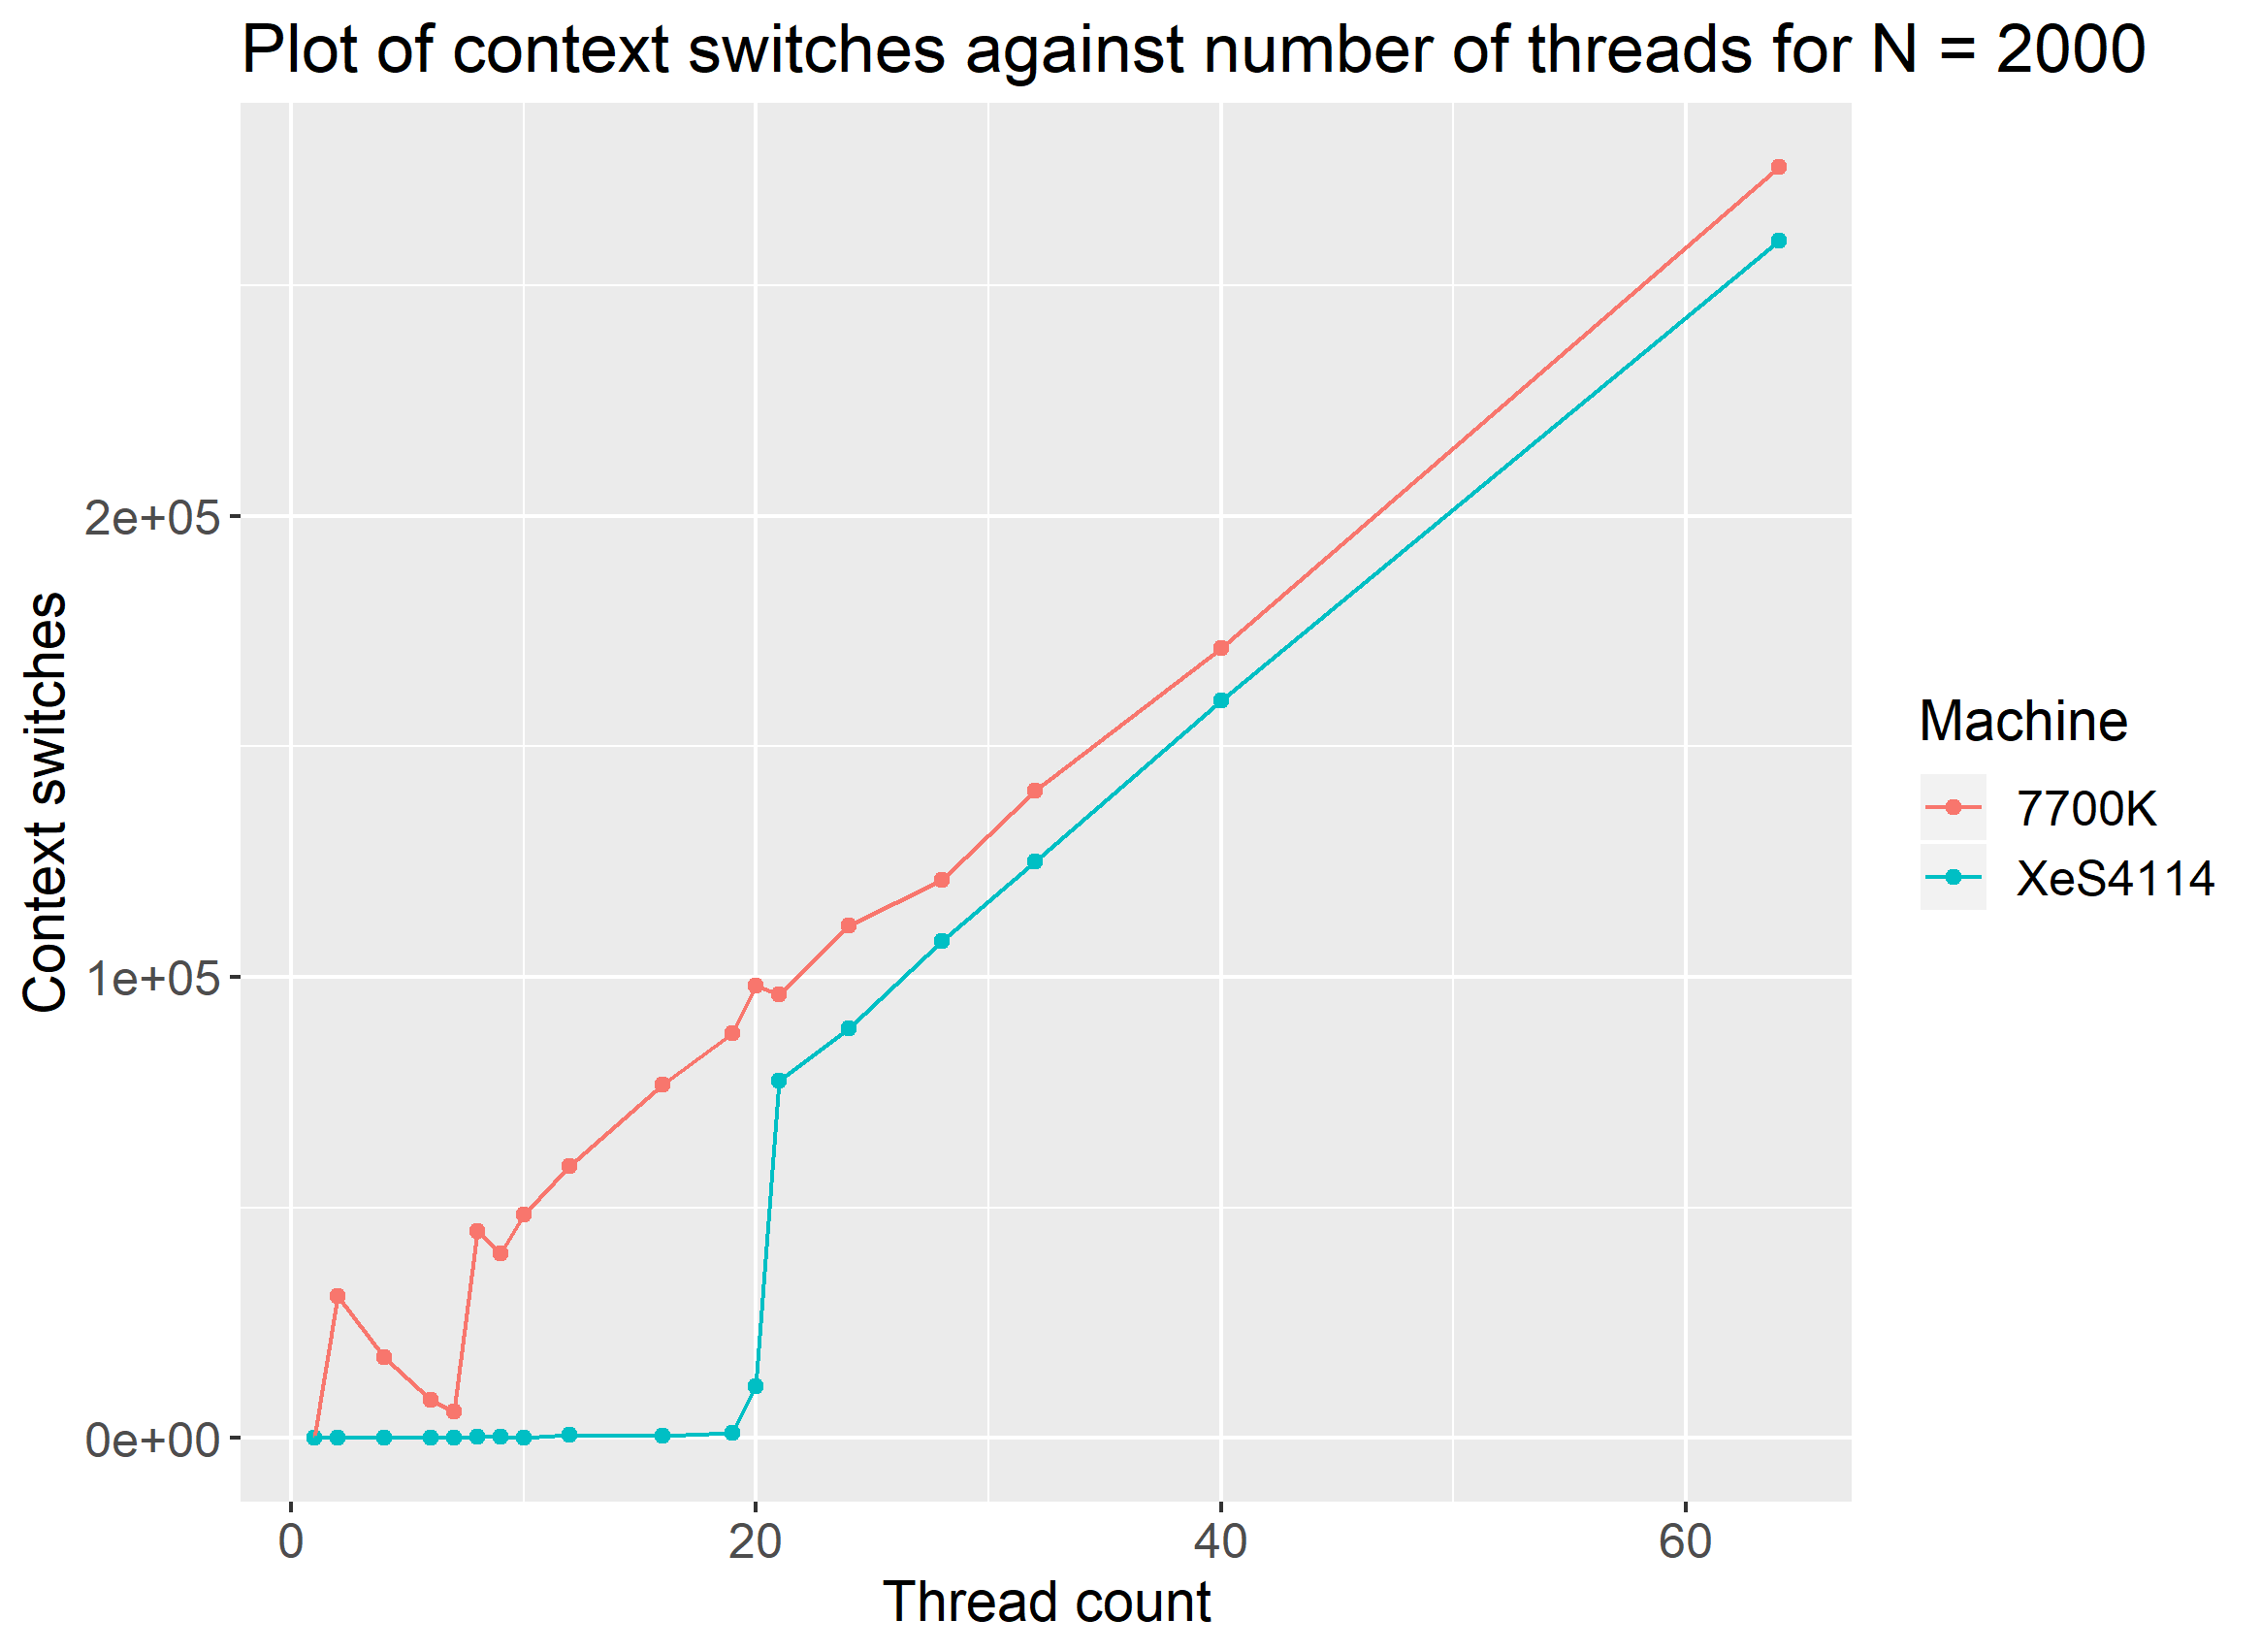
\includegraphics[width=0.75\textwidth]{par-2000N-contextSwitches}
    \caption{Plot of number of context switches against number of threads $T$ for $N = 2000$}
    \label{fig:par-2000N-contextSwitches}
\end{figure}

\pagebreak

\section{Discussion: Sequential Implementation}

\subsection{Expectations} \label{seq-expect}

For a single step in the simulation, the different components contribute different amounts to the execution time for that step:
\begin{itemize}
	\item Checking $\Theta(N^2)$ potential collisions, each incurring a cost of $T_{check}$: $O(N^2)T_{check}$
	\item Sorting $\Theta(N)$ collisions (since we assume $P(collision) \ll 1$): $O(N log N)$
	\item Resolving $\Theta(N)$ collisions (since each particle is involved in at most one collision), each incurring a cost of $T_{resolve}$: $O(N)T$
	\item Updating positions of particles not involved in any collisions: $O(N)$
\end{itemize}

Thus, the execution time per step is $O(N^2)$, since $T_{check}$ is constant $\implies$ the overall execution time is $O(N^2S)$. \\

Hence, we expect that the overall execution time is dominated by the work required for the collision checking stage.

\subsection{Conclusions}

From Figure \ref{fig:seq-varyN}, we see that the execution time increases quadratically with the number of particles $N$, which agrees with our expectations in (\ref{seq-expect}). \\

From Figure \ref{fig:seq-varyL}, we observe that the execution time appears to be constant with respect to the size of the box $L$. Increasing $L$ increases the initial velocity limit of particles and reduces the average particle density – reducing the number of particle-wall collisions but not the number of particle-particle collisions. \\

From Figure \ref{fig:seq-varyR}, we also observe that the radius of particles does not appear to influence the execution time. Even when the radius of particles is $r=16$, particles still only occupy a negligible fraction of the total area of the square, thus the total number of particle-particle collisions does not rise appreciably relative to the number of particle-wall collisions. \\
\begin{itemize}
	\item Changing either $L$ or $r$ does not change the amount of work performed in checking collisions for each step, hence they rightfully do not affect the overall execution time.
\end{itemize}

From Figure \ref{fig:seq-varySteps}, the execution time appears to grow linearly with the number of steps $S$ of the simulation. For a random simulation, the average number of collision per time steps should be similar, and all $\Theta(N^2)$ potential collisions are checked per time step. Thus, the computation work done per time step is approximately equal, and hence this agrees with our expectations in (\ref{seq-expect}). \label{seq-linear-growth-steps} \\

Of the above results, only the dependence of execution time on the number of particles $N$ was notable. Hence, for the parallel implementations, we opted to only vary $N$ amongst the simulation parameters.

\pagebreak

\section{Discussion: Parallel Implementation}

\subsection{Expectations}

We expected our parallel implementation to demonstrate an increasing speedup over the sequential implementation with an increasing number of threads $T$, up to an optimum number of threads $T_{opt}$. This is because we employed dynamic scheduling to distribute work equitably amongst the OpenMP threads.

\subsection{Conclusions}

From Figures \ref{fig:par-250N-varyThreads} - \ref{fig:par-2000N-varyThreads}, we observed that the execution time for a fixed $N$ generally decreases with an increasing number of threads $T$, up to an optimum number of $T$. Here, the optimal number of threads $T_{opt}$ is shown for the Intel i7-7700K and Xeon Silver 4114, which have 8 and 20 logical cores respectively.

\begin{center}
	\begin{tabular}{ | c | c | c | }
		\hline
		N & Optimal $T$ for i7-7700K & Optimal $T$ for Xeon 4114 \\ \hline
		250 & 7 & 16 \\ \hline
		500 & 7 & 21 \\ \hline
		1000 & 7 & 21 \\ \hline
		2000 & 7 & 21 \\ \hline
	\end{tabular}
\end{center}

For both processors and all $N$ tested, the optimal number of threads $T_{opt}$ was not equal to the number of logical cores they possessed. We hypothesise this occurs due to scheduling issues and contention over hardware resources, since Figure \ref{fig:par-2000N-contextSwitches} shows that the number of expensive context-switches begins to rapidly increase when the number of threads $T$ is 1 less than the number of logical cores of that processor. \\

Notably, when $T$ is equal to the number of logical cores, the overall execution time degrades significantly, to performance that is sometimes worse than the sequential implementation. This is despite us ensuring no other concurrent processes were running on the nodes when the testcases were being executed.

\begin{center}
	\begin{tabular}{ | c | c | c | }
		\hline
		N & Maximum $s$ for i7-7700K & Maximum $s$ for Xeon 4114 \\ \hline
		250 & 4.6 & 6.0 \\ \hline
		500 & 5.0 & 8.8 \\ \hline
		1000 & 6.0 & 11.5 \\ \hline
		2000 & 6.0 & 11.9 \\ \hline
	\end{tabular}
\end{center}

From Figures \ref{fig:par-250N-speedup} - \ref{fig:par-2000N-speedup}, we also observe the trend that the maximum speedup $s$ (rounded to 1 d.p.) over the sequential implementation increases with the number of particles $N$. This is expected since the bulk of the computational work performed by the simulation occurs during the (parallelised) collision checking stage, which increases rapidly with $N$. \\

Additionally, we also expected that the peak speedup will not equate the total number of logical cores of a processor, due to three reasons. First, not all of the work in each simulation step is parallelised, as there remains serial portions (e.g. filtering of collision candidates). Next, the work of collision checking may not be distributed equally amongst the threads despite dynamic scheduling, since faster particles have a greater probability to collide with walls or other particles. Third, the critical section also results in some threads blocking whilst waiting to add a new collision candidate to the array.

\subsection{Benefits of discrete simulation}

Discrete simulation with arbitrary time-units possesses a benefit over execution-time units, in that we can avoid introducing additional floating-point errors associated with simulating with execution-time units. Furthermore, it simplifies the simulation since the state of all particles in the following step can be directly computed from their states in the previous step.

\pagebreak

\section{Early-pruning Optimisation}

\subsection{Motivation}

From our two initial implementations, we observe that the most computationally expensive section of our simulation lies in checking collisions between particles, since there are
$$ N_{particle-particle} = \begin{pmatrix} N \\ 2 \end{pmatrix} = \frac{N(N-1)}{2}$$
such potential collisions, each requiring the entire computation on page \pageref{trajectory-calc}. \\

Therefore, to optimise the simulation, we propose that it is possible to perform early pruning of impossible particle collision pairs, to avoid this expensive computation whilst \ul{preserving correctness}.

\subsection{Implementation}

Let us suppose all particles are bounded by a speed limit $v_{limit}$. Consider a particle $P$ at a given location ($x$,$y$) in the square at the beginning of a time step. \\

\begin{figure}[H]
    \centering
    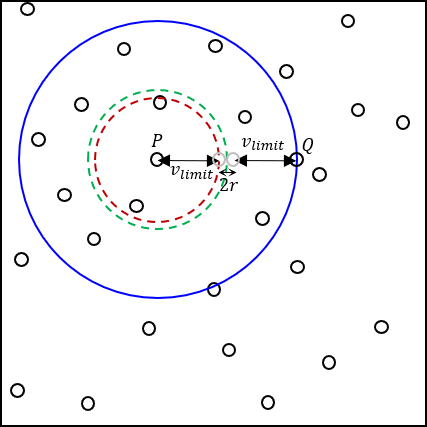
\includegraphics[width=0.5\textwidth]{chap8RadOfCollision}
    \caption{Radius of collision (blue circle) for a given particle}
    \label{fig:chap8RadOfCollision}
\end{figure}

For this time step, only particles within the blue circle of radius $R=2v_{limit}+2r$ centered on $P$ can possibly collide with $P$. All other particles are too great a distance away to collide during this time step. \\

In the worst case, both particles $P$, $Q$ are initially at a distance of $d=2v_{limit}+2r$ at the start, travel $v_{limit}$ units towards each other during the time step, and collide at a distance of $d=2r$ at the end of the time step. This corresponds to the pair of grey particles along the dotted green border in Figure \ref{fig:chap8RadOfCollision}. \\

To achieve this, we first sub-divide the square into a grid containing $G \times G$ equally sized cells, each of dimension
$$w = \frac{L}{G}$$

For each step of the simulation, we assign a particle a given cell ID based on its coordinates ($x$,$y$), comprising a pair of integer coordinates ($G_x$,$G_y$). We do this by
$$G_x = \left\lfloor{\frac{x}{w}}\right\rfloor, G_y = \left\lfloor{\frac{y}{w}}\right\rfloor$$

Then, we can approximate the set of potential particles $P$ can collide with, by only checking particles in cells within the red square $S$ (which intersect some part of the blue circle). \\

\begin{figure}[H]
    \centering
    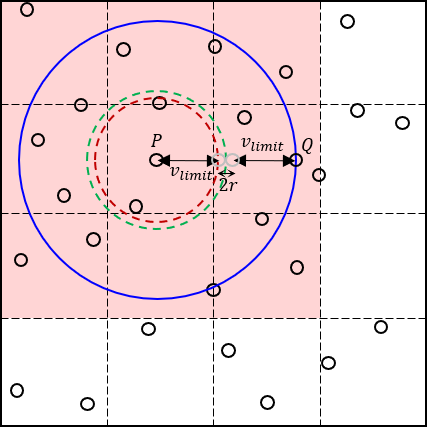
\includegraphics[width=0.5\textwidth]{chap8ApproxCollision}
    \caption{Approximate set of potential particle collision partners $G$ for a particle $P$}
    \label{fig:chap8ApproxCollision}
\end{figure}

However, since a particle can be located anywhere within a grid cell G, we need to include additional cells surrounding the red square into the final set of cells S', which is highlighted by the yellow region here. \\

\begin{figure}[H]
    \centering
    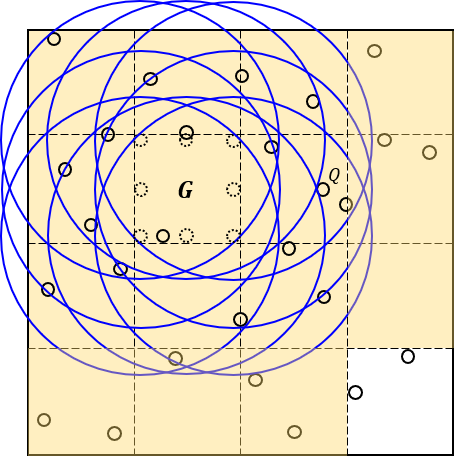
\includegraphics[width=0.5\textwidth]{chap8ExpandedSet}
    \caption{Expanded set of potential particle collision partners $G$ for a particle $P$}
    \label{fig:chap8ExpandedSet}
\end{figure}

To determine if a cell $G'$ is contained within $S'$, we use the Manhattan distance $d_M$ between the target cell $G$ and $G'$. \\

We compute the maximum Manhattan distance between the target grid cell $G$ and a cell in $S'$,
$$d_{M\_max} = \left\lceil{\frac{R}{w}}\right\rceil = \left\lceil{\frac{2v_{limit} + 2r}{w}}\right\rceil$$

Then, for each particle-collision pair ($P$,$Q$) in each time step, we first compute the Manhattan distance between the cells $G_P$ and $G_Q$ these two particles belong to,
$$\Delta d_M=\left| G_{Q,x} - G_{P,x} \right| + \left| G_{Q,y} - G_{P,y} \right|$$

If $d_M \leq d_{M\_max}$, the two particles belong to grid cells that are sufficiently close, and thus these particles may collide during this time step. For such particle-collision pairs, we solve their trajectory equations as per page \pageref{trajectory-calc}. \\

Otherwise, $d_M > d_{M\_max}$, and we immediately return \ul{no collision} for ($P$, $Q$).

\subsection{First results}

We modified our parallel implementation (in folder \texttt{/code/parallel}) to include this early-pruning optimisation (in \texttt{/code/parallel-2}), with $v_{limit}$ set to one-quarter the dimension of the box. We ran both parallel implementations with the default test case (simulation parameters $N=1000, L=20000, r=1, S=1000$) and compared the final state of the simulation, to check correctness. \\

However, we noticed that both implementations did not converge to the same final state of the simulation. Further inspection showed that the state of the simulation between both implementations diverged very early near the beginning of the simulation.

\subsection{Velocity anomalies}

We examined closely the output from running the parallel implementation (which we assume is correct) with the default testcase in \bt{print} mode. We noticed that, early in the simulation, some particles were already exceeding our specified velocity limit
$$v_{limit} = \frac{L}{4}$$

which meant that the early-pruning optimisation incorrectly pruned particle-collision pairs involving such fast particles. \\

We wrote a Python script (\texttt{/anomalies/veloDetect.py}) to examine the output of the default testcase in \bt{print} mode, and found that such violations were numerous. The results of the script are found in \texttt{/anomalies/stdAnalysis.txt}. \\

For the default testcase with $N=1000$ and $S=1000$, there were a total of 177927 recorded instances where the magnitude of a particle’s velocity exceeded $v_{limit}$. This shows that on average, about 17.8\% of particles during a given time step had velocities $\left|v\right| \geq v_{limit}$. \\

Additionally, the maximum velocity of a particle recorded over the entire simulation was $\left|v\right|_{max} = 13007$ units/step, a staggering 160\% greater than the speed limit of $v_{limit} = L/4 = 5000$ units/step. \\

Therefore, the assumption that particles in the box obey a velocity limit $v_{limit}$ needs to be re-examined.

\subsection{Bounding the velocity limit}

For particles, we observe that the \ul{magnitude} of their velocity only changes during particle-particle elastic collisions, since particle-wall collisions only changes the direction of motion. \\

Suppose the particles within the box obey some velocity limit $v_{limit}$. Consider an orthogonal collision involving two particles $P$, $Q$ travelling at or near $v_{limit}$, as in Figure \ref{fig:chap8Slingshot}. \\

\begin{figure}[H]
    \centering
    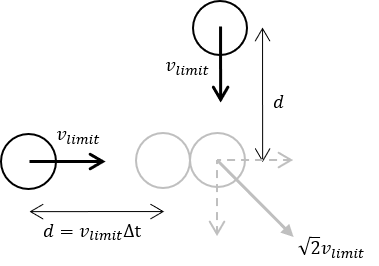
\includegraphics[width=0.5\textwidth]{chap8Slingshot}
    \caption{``Slingshot'' effect from orthogonal particle-particle collisions}
    \label{fig:chap8Slingshot}
\end{figure}

Since the two particles collide elastically, particle $Q$ will transfer all its momentum to particle $P$ and stop entirely ($v_Q' = 0$). Hence, particle $P$ possesses a final velocity
$$v'_P = \sqrt{v_{P_x}^{'2} + v_{P_y}^{'2}} = \sqrt{v_{limit}^2 + v_{limit}^2} = \sqrt{2}v_{limit}$$

that exceeds $v_{limit}$. As a result, particle $P$ may collide with other particles beyond the specified yellow region in the next time step, but such a collision will be incorrectly discarded by the optimisation. \\

In effect, particles colliding at near right-angles to each other will result in a massive transfer of momentum to one of the particles, ``slingshotting" it far beyond the initial velocities of either particle. \\

Therefore, it seems that there is no upper bound to the velocity of particles within the box. However, since elastic collisions conserve kinetic energy, the highest velocity a particle can attain remains bounded by the total kinetic energy of all particles in the box. \\

Suppose for the $i$th particle that it began the simulation with velocity of $v_i \le v_{limit}$, then the total kinetic energy in the box is
\begin{align*}
	E_K 	&= \sum_{i=1}^N mv_i^2 = m \sum_{i=1}^N v_i^2 \\
		&\leq m \sum_{i=1}^N v_{limit}^2 = mNv_{limit}^2
\end{align*}

Therefore, the maximum velocity of a partciel in the box, which occurs when it possesses all the kinetic energy and all other particles are stationary, is
$$ v_{max} = \sqrt{\frac{2E_K}{m}} = \sqrt{\frac{2mNv_{limit}^2}{m}} = \sqrt{2N}v_{limit} $$

which is dependent on $N$ and the initialisation velocity limit $v_{limit}$.

\subsection{Reducing particle velocities}

\begin{figure}[H]
    \centering
    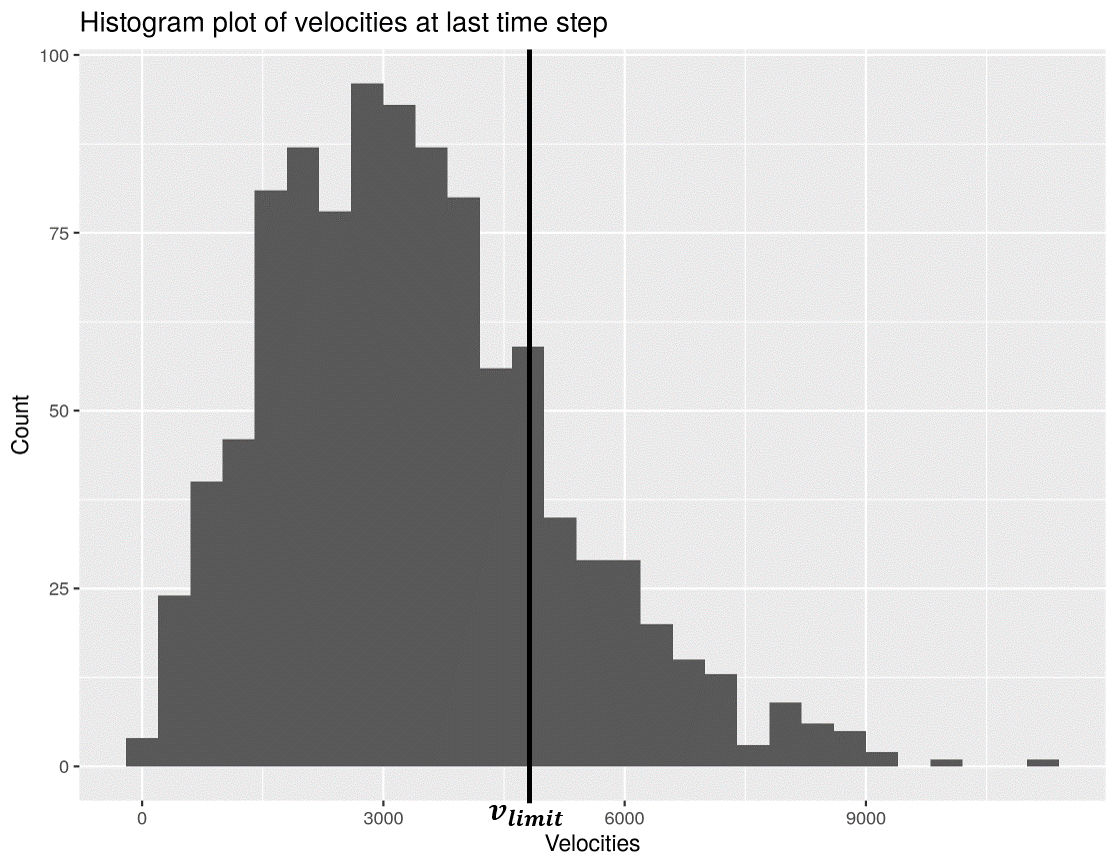
\includegraphics[width=0.75\textwidth]{chap8Velocities}
    \caption{Plot of particles against velocity at final step (bin size: 400 units/step)}
    \label{fig:chap8Velocities}
\end{figure}

We observe, however, that whilst particles may exceed $v_{limit} = L/4$, the probability of greater violations decreases with increasing final velocity. Since the particles in the box collide randomly, it requires a much longer sequence of collisions to build up a particle to a much greater velocity above $v_{limit}$, as compared to a particle that exceeds $v_{limit}$ only by a small amount. \\

This hypothesis is verified by the plot in Figure \ref{fig:chap8Velocities}, which shows that bulk of the particles remain below $v_{limit}$, and that amongst the particles that exceed $v_{limit}$, the frequency of such particles decreases with increasing $v$. Notably, the uniform random distribution of particle velocities the simulation began with evolved into a Boltzmann-like distribution at the end of the simulation. \\

Therefore, we propose that this early-pruning optimisation may still be applied to obtain an improvement in execution time, by reducing the typical velocities of particles. This will be achieved by setting the value of \texttt{SLOW\_FACTOR} to 4 (see page \pageref{slow-factor-ref}). In effect, this reduces the velocity of particles in units/step by a factor of 4, whilst quadrupling the total number of steps in the simulation, i.e. each initial step is replaced by four smaller ``micro-steps''. \\

This has the side-effect of increasing the granularity and accuracy of the simulation, at the cost of approximately 4 times the runtime (see page \pageref{seq-linear-growth-steps}). With this modification, we checked the output for a variety of testcases (varying $N$ and $s$), and verified that all three implementations converge to the same final simulation state.

\subsection{Test setup for early-pruning optimisation}

To examine the effect of this optimisation, we re-ran a modified version of the default testcase for all three implementations, but with the \texttt{SLOW\_FACTOR} set to 4. This was done as the previous data collected was for a different simulation granularity (\texttt{SLOW\_FACTOR} of 1), and thus should not be used for direct comparisons. \\

In contrast with previous runs, we ran the Bash script in the background, and made the process ignore the \texttt{SIGHUP} (hangup) signal. The full shell command used is \bt{nohup ./<impl>BatchRun.sh \&}. \\

The simulation parameters of the modified default testcase is
\begin{itemize}
	\item $\textbf{N = 2000}, L = 20000, r = 1, S = 1000, \texttt{SLOW\_FACTOR}$ set to 4
\end{itemize}

The test cases that were executed for each implementation are as follows:
\begin{enumerate}
	\item \textbf{Sequential implementation}: modified default test case only
	\item \textbf{Parallel implementation}
		\begin{itemize}
			\item $T$ = number of OpenMP threads
			\item Varying $T$ only: $T = 1, 2, 4, 6, 7, 8, 9, 10, 12, 16, 19, 20, 21, 24, 32, 40, 64$
		\end{itemize}
	\item \textbf{Early-pruning parallel implementation}
		\begin{itemize}
			\item $G$ = grid dimension in cells per box length
			\item Varying both T and G together
				\begin{itemize}
					\item $T = 1, 2, 4, 6, 7, 8, 9, 10, 12, 16, 19, 20, 21, 24, 28, 32, 40, 64$
					\item $G = 1, 2, 4, 8, 16, 32, 64$
				\end{itemize}
		\end{itemize}
\end{enumerate}

\subsection{Processed results}

The raw data for this new dataset is available in \texttt{/data/parallelVsParallel2}. Only the plots for speedup are reproduced here; the remaining plots for execution time are found as \texttt{.png} image files in \texttt{/data/parallelVsParallel2}. \\

The dotted and solid curves represent the speedup of the parallel and early-pruning parallel implementations respectively, relative to the sequential implementation.

\begin{figure}[H]
    \centering
    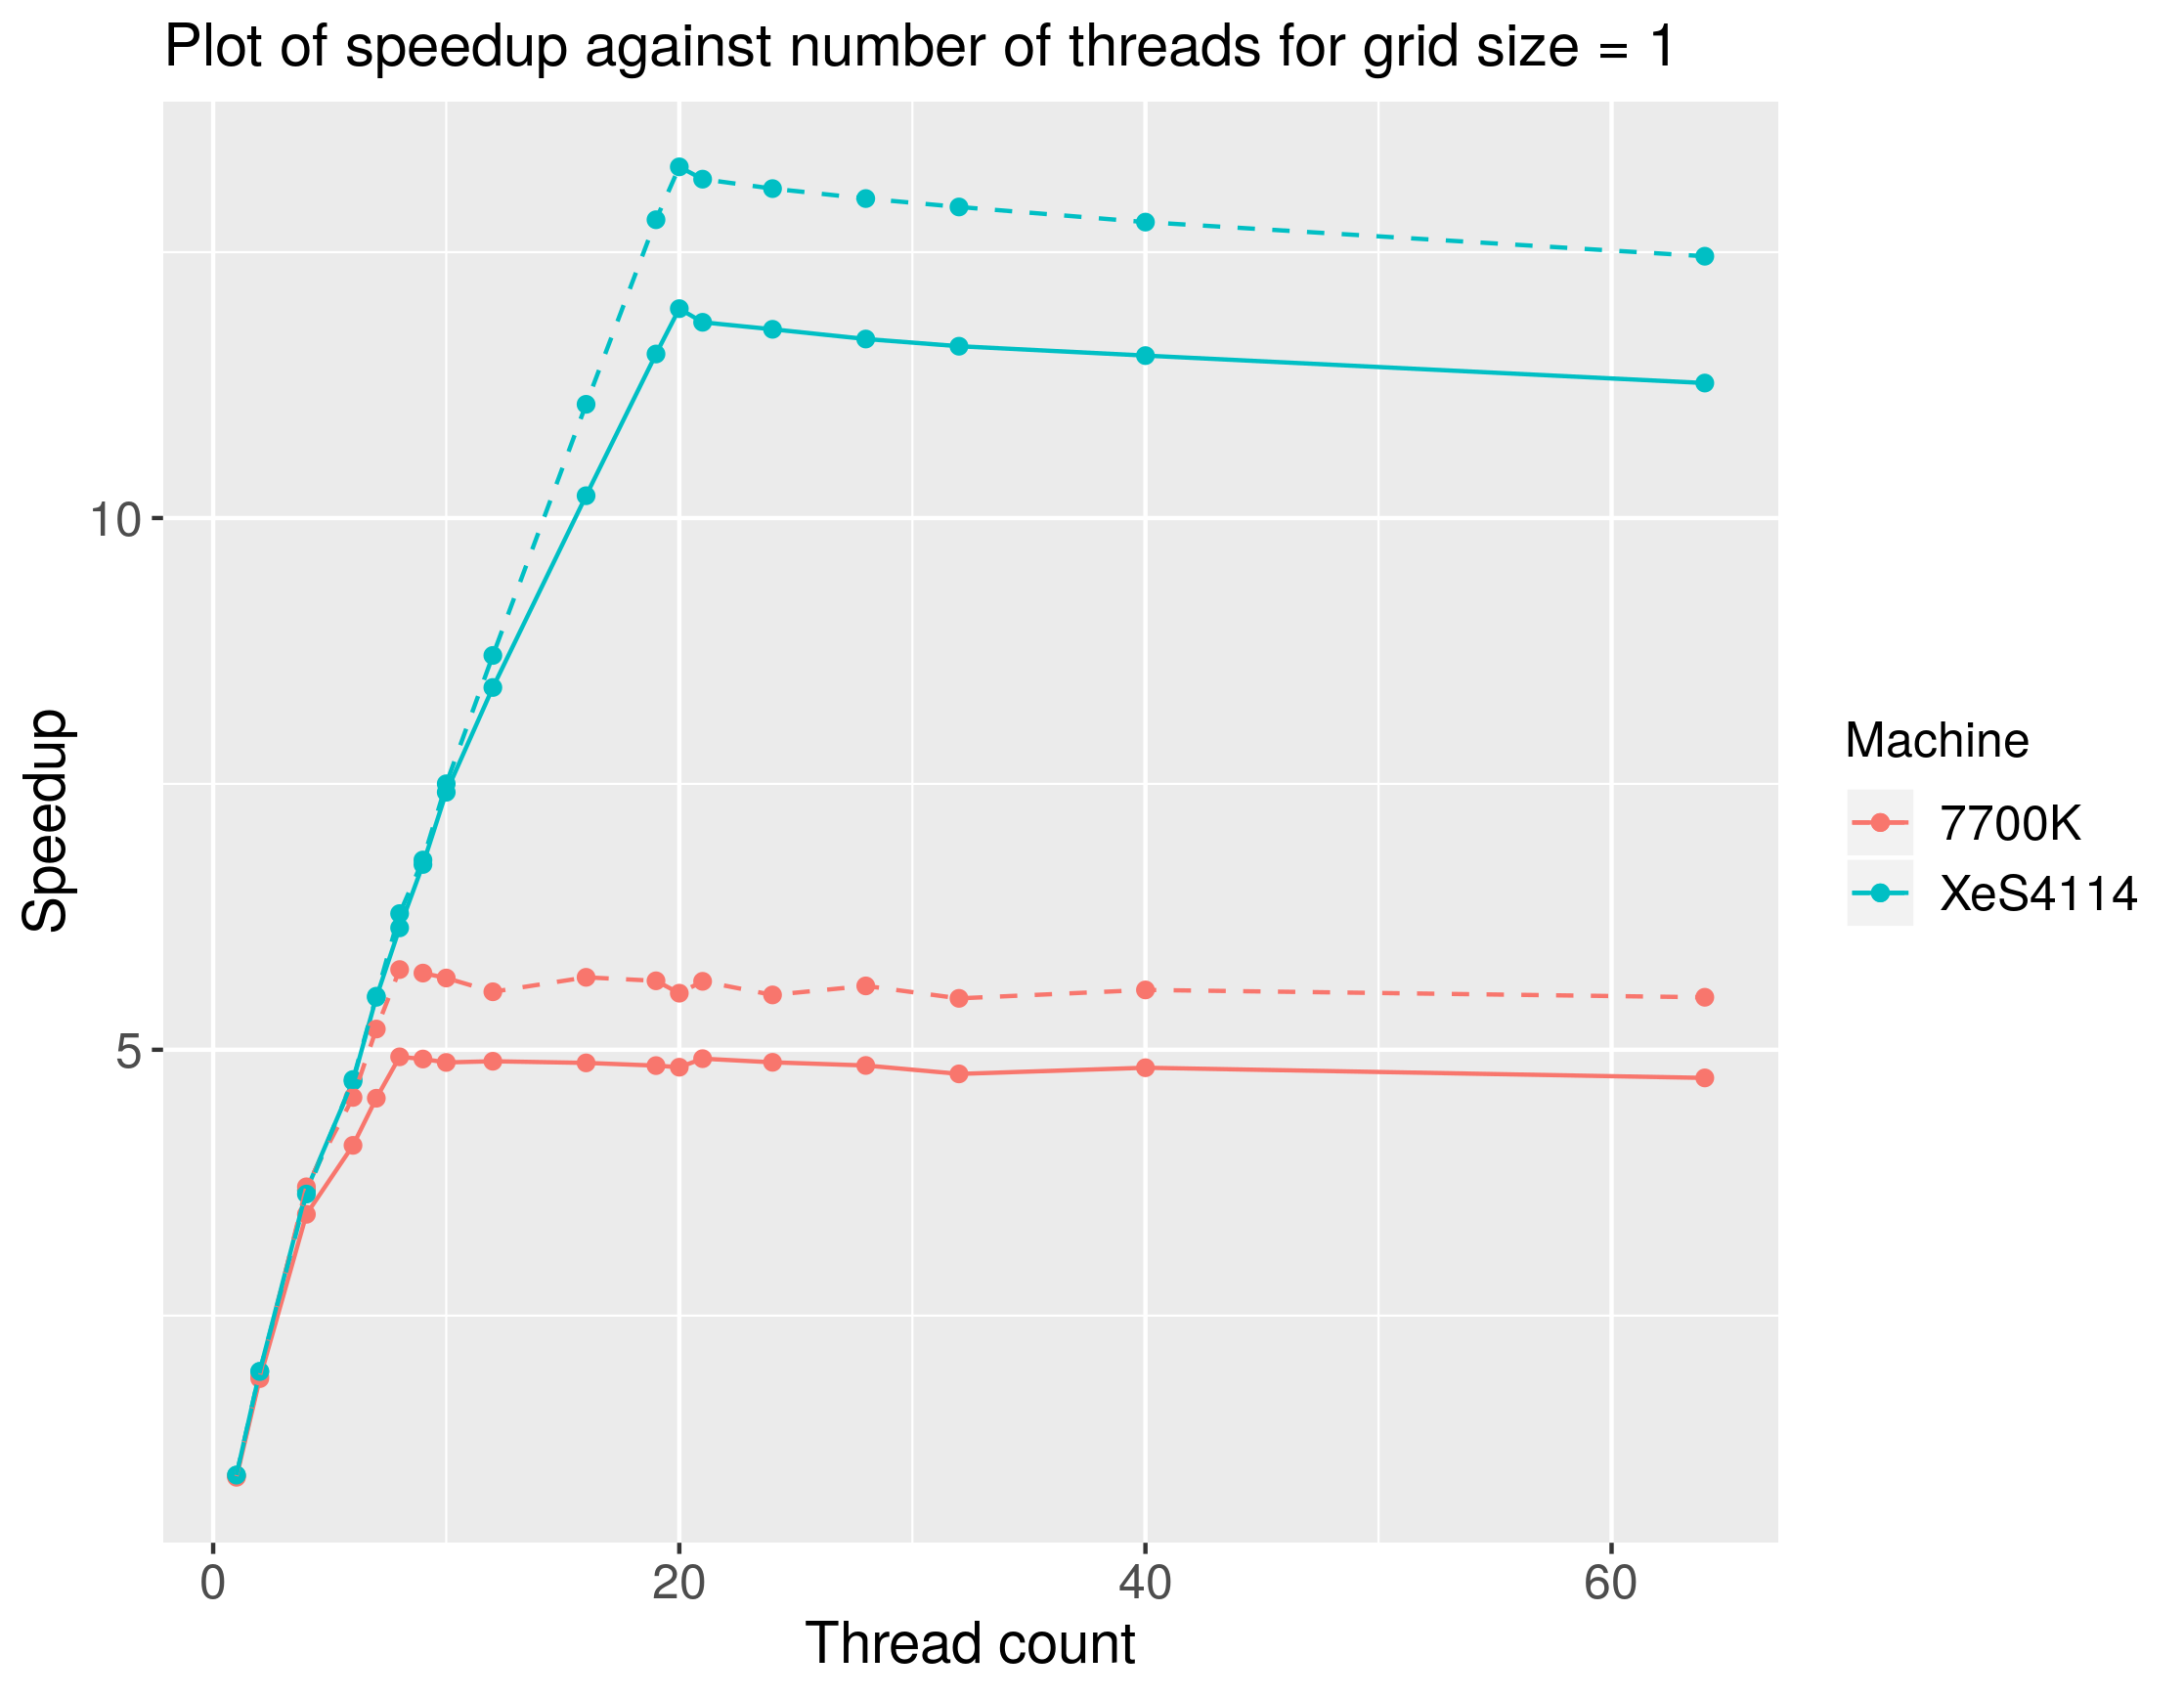
\includegraphics[width=0.75\textwidth]{optPar-gridSize1-speedup}
    \caption{Plot of speedup against number of threads $T$ for grid size of $G = 1$}
    \label{fig:optPar-gridSize1-speedup}
\end{figure}

\begin{figure}[H]
    \centering
    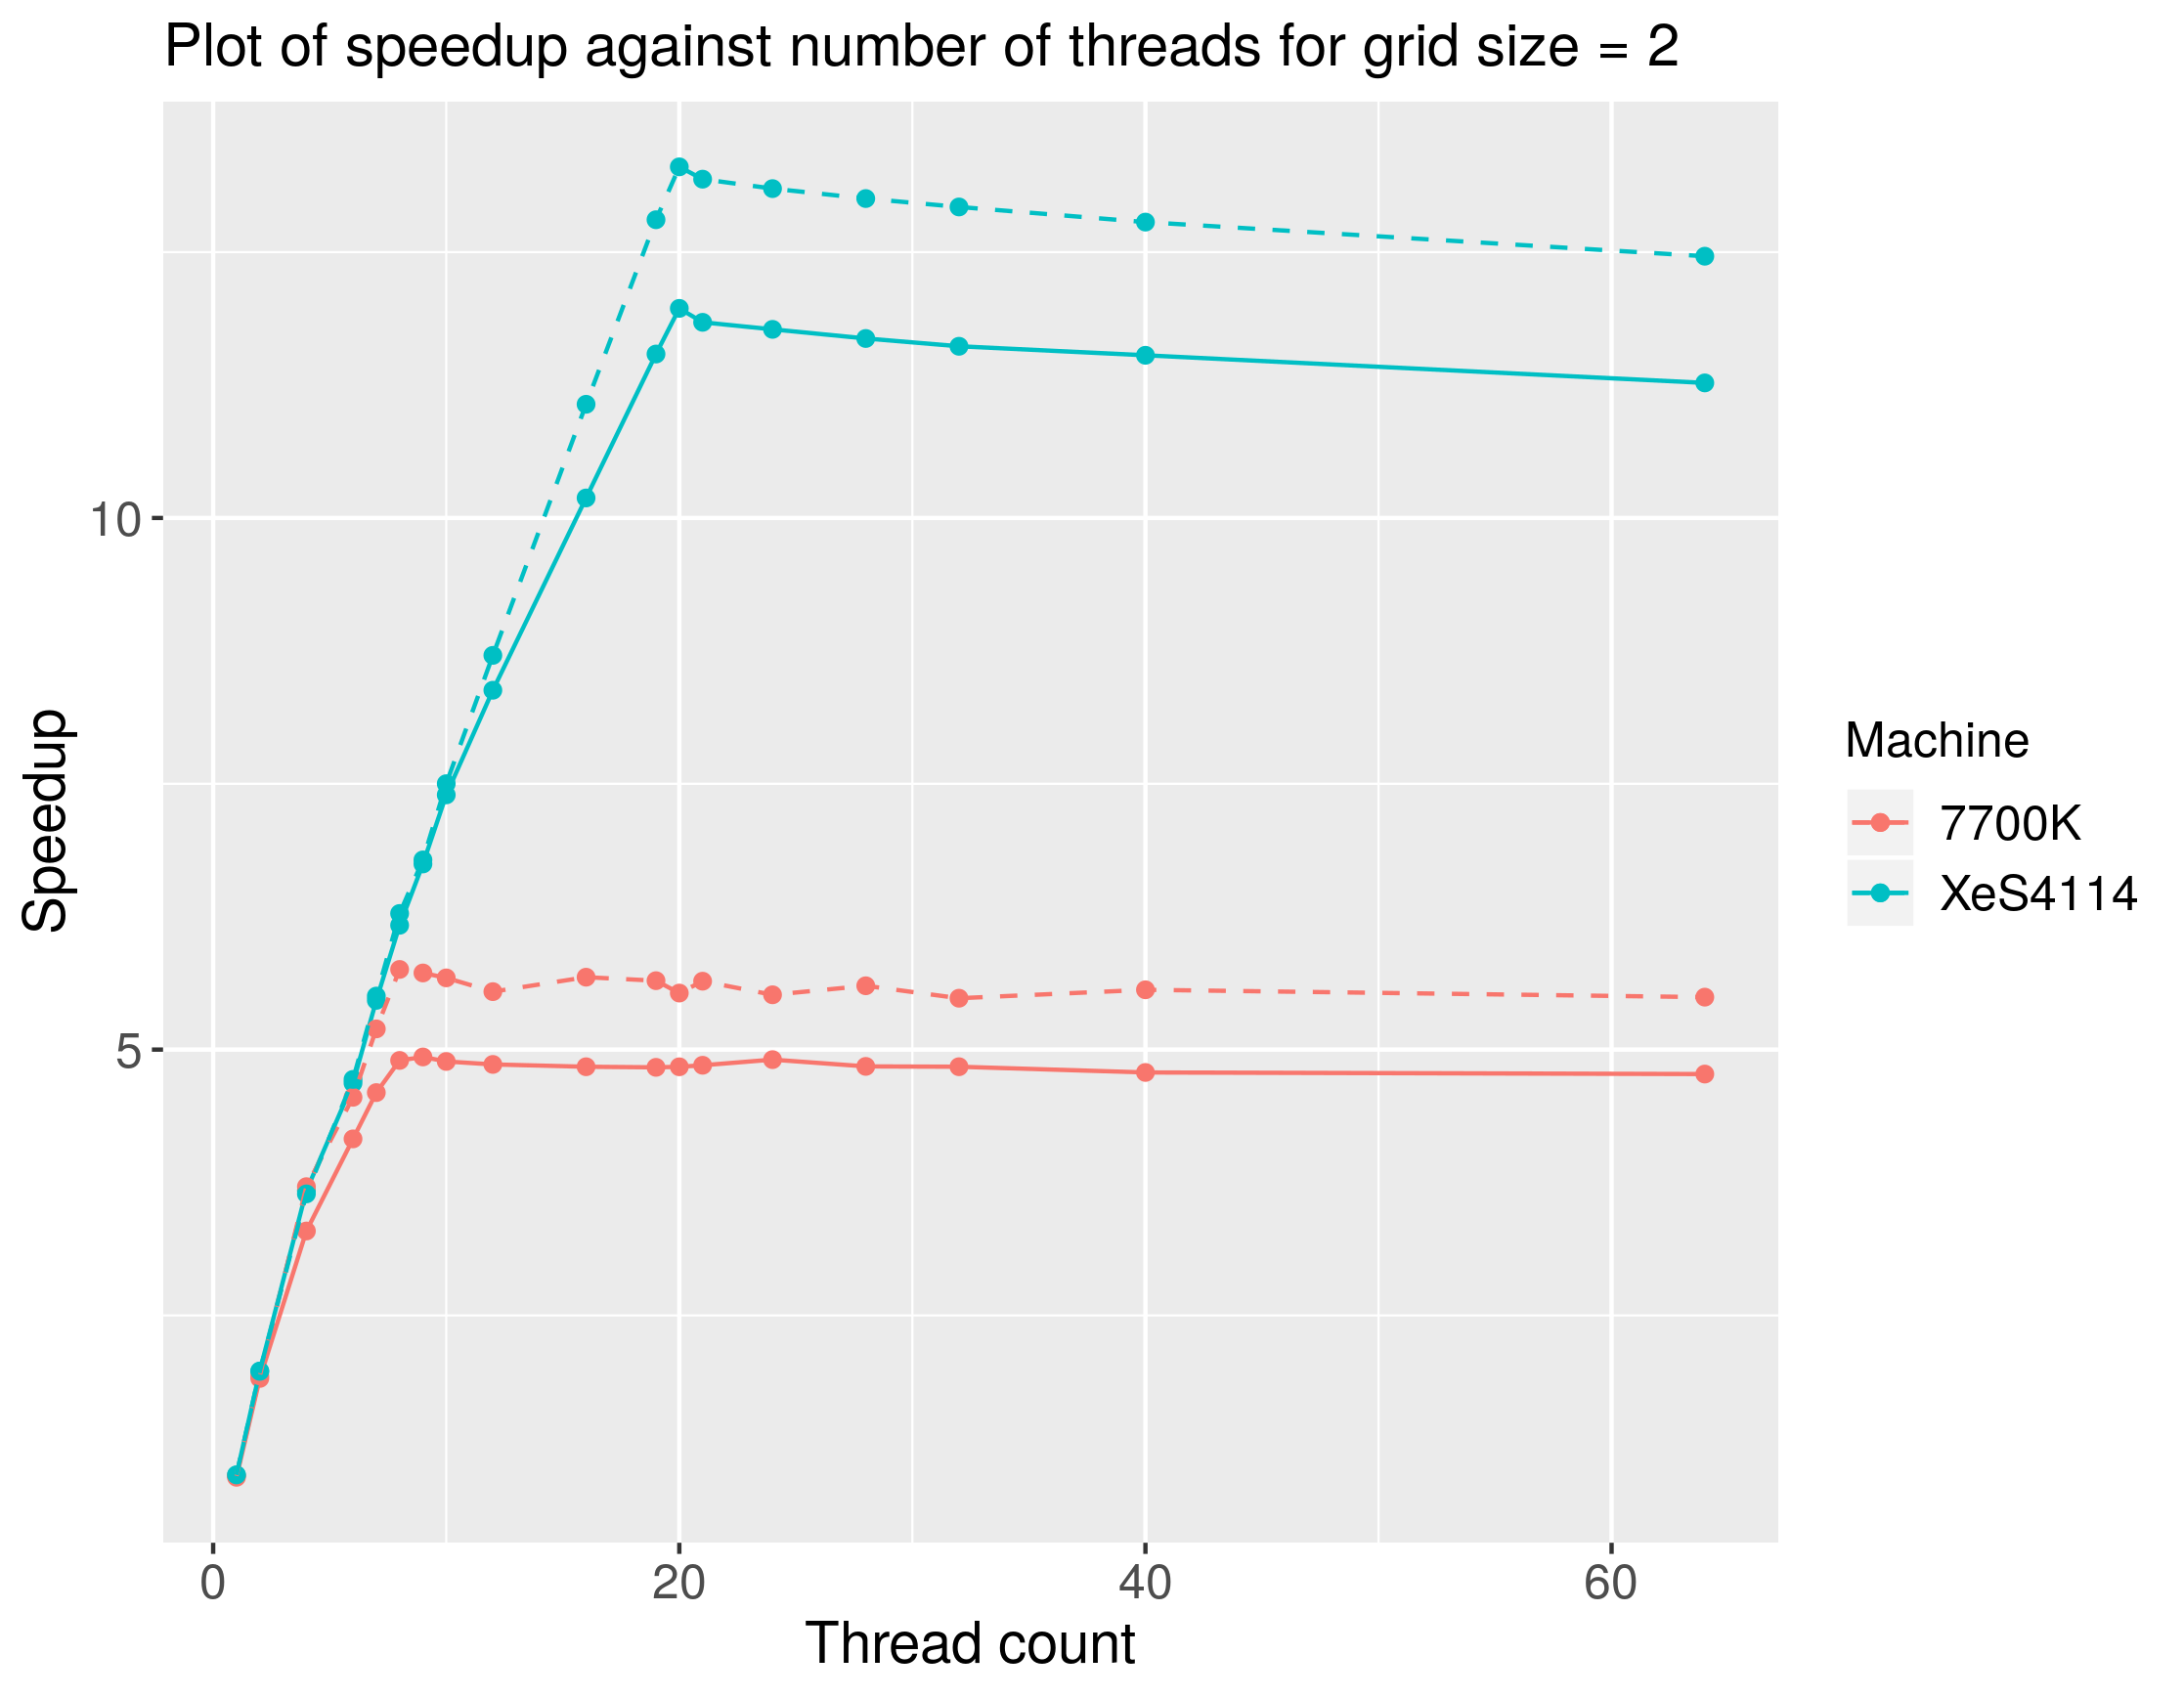
\includegraphics[width=0.75\textwidth]{optPar-gridSize2-speedup}
    \caption{Plot of speedup against number of threads $T$ for grid size of $G = 2$}
    \label{fig:optPar-gridSize2-speedup}
\end{figure}

\begin{figure}[H]
    \centering
    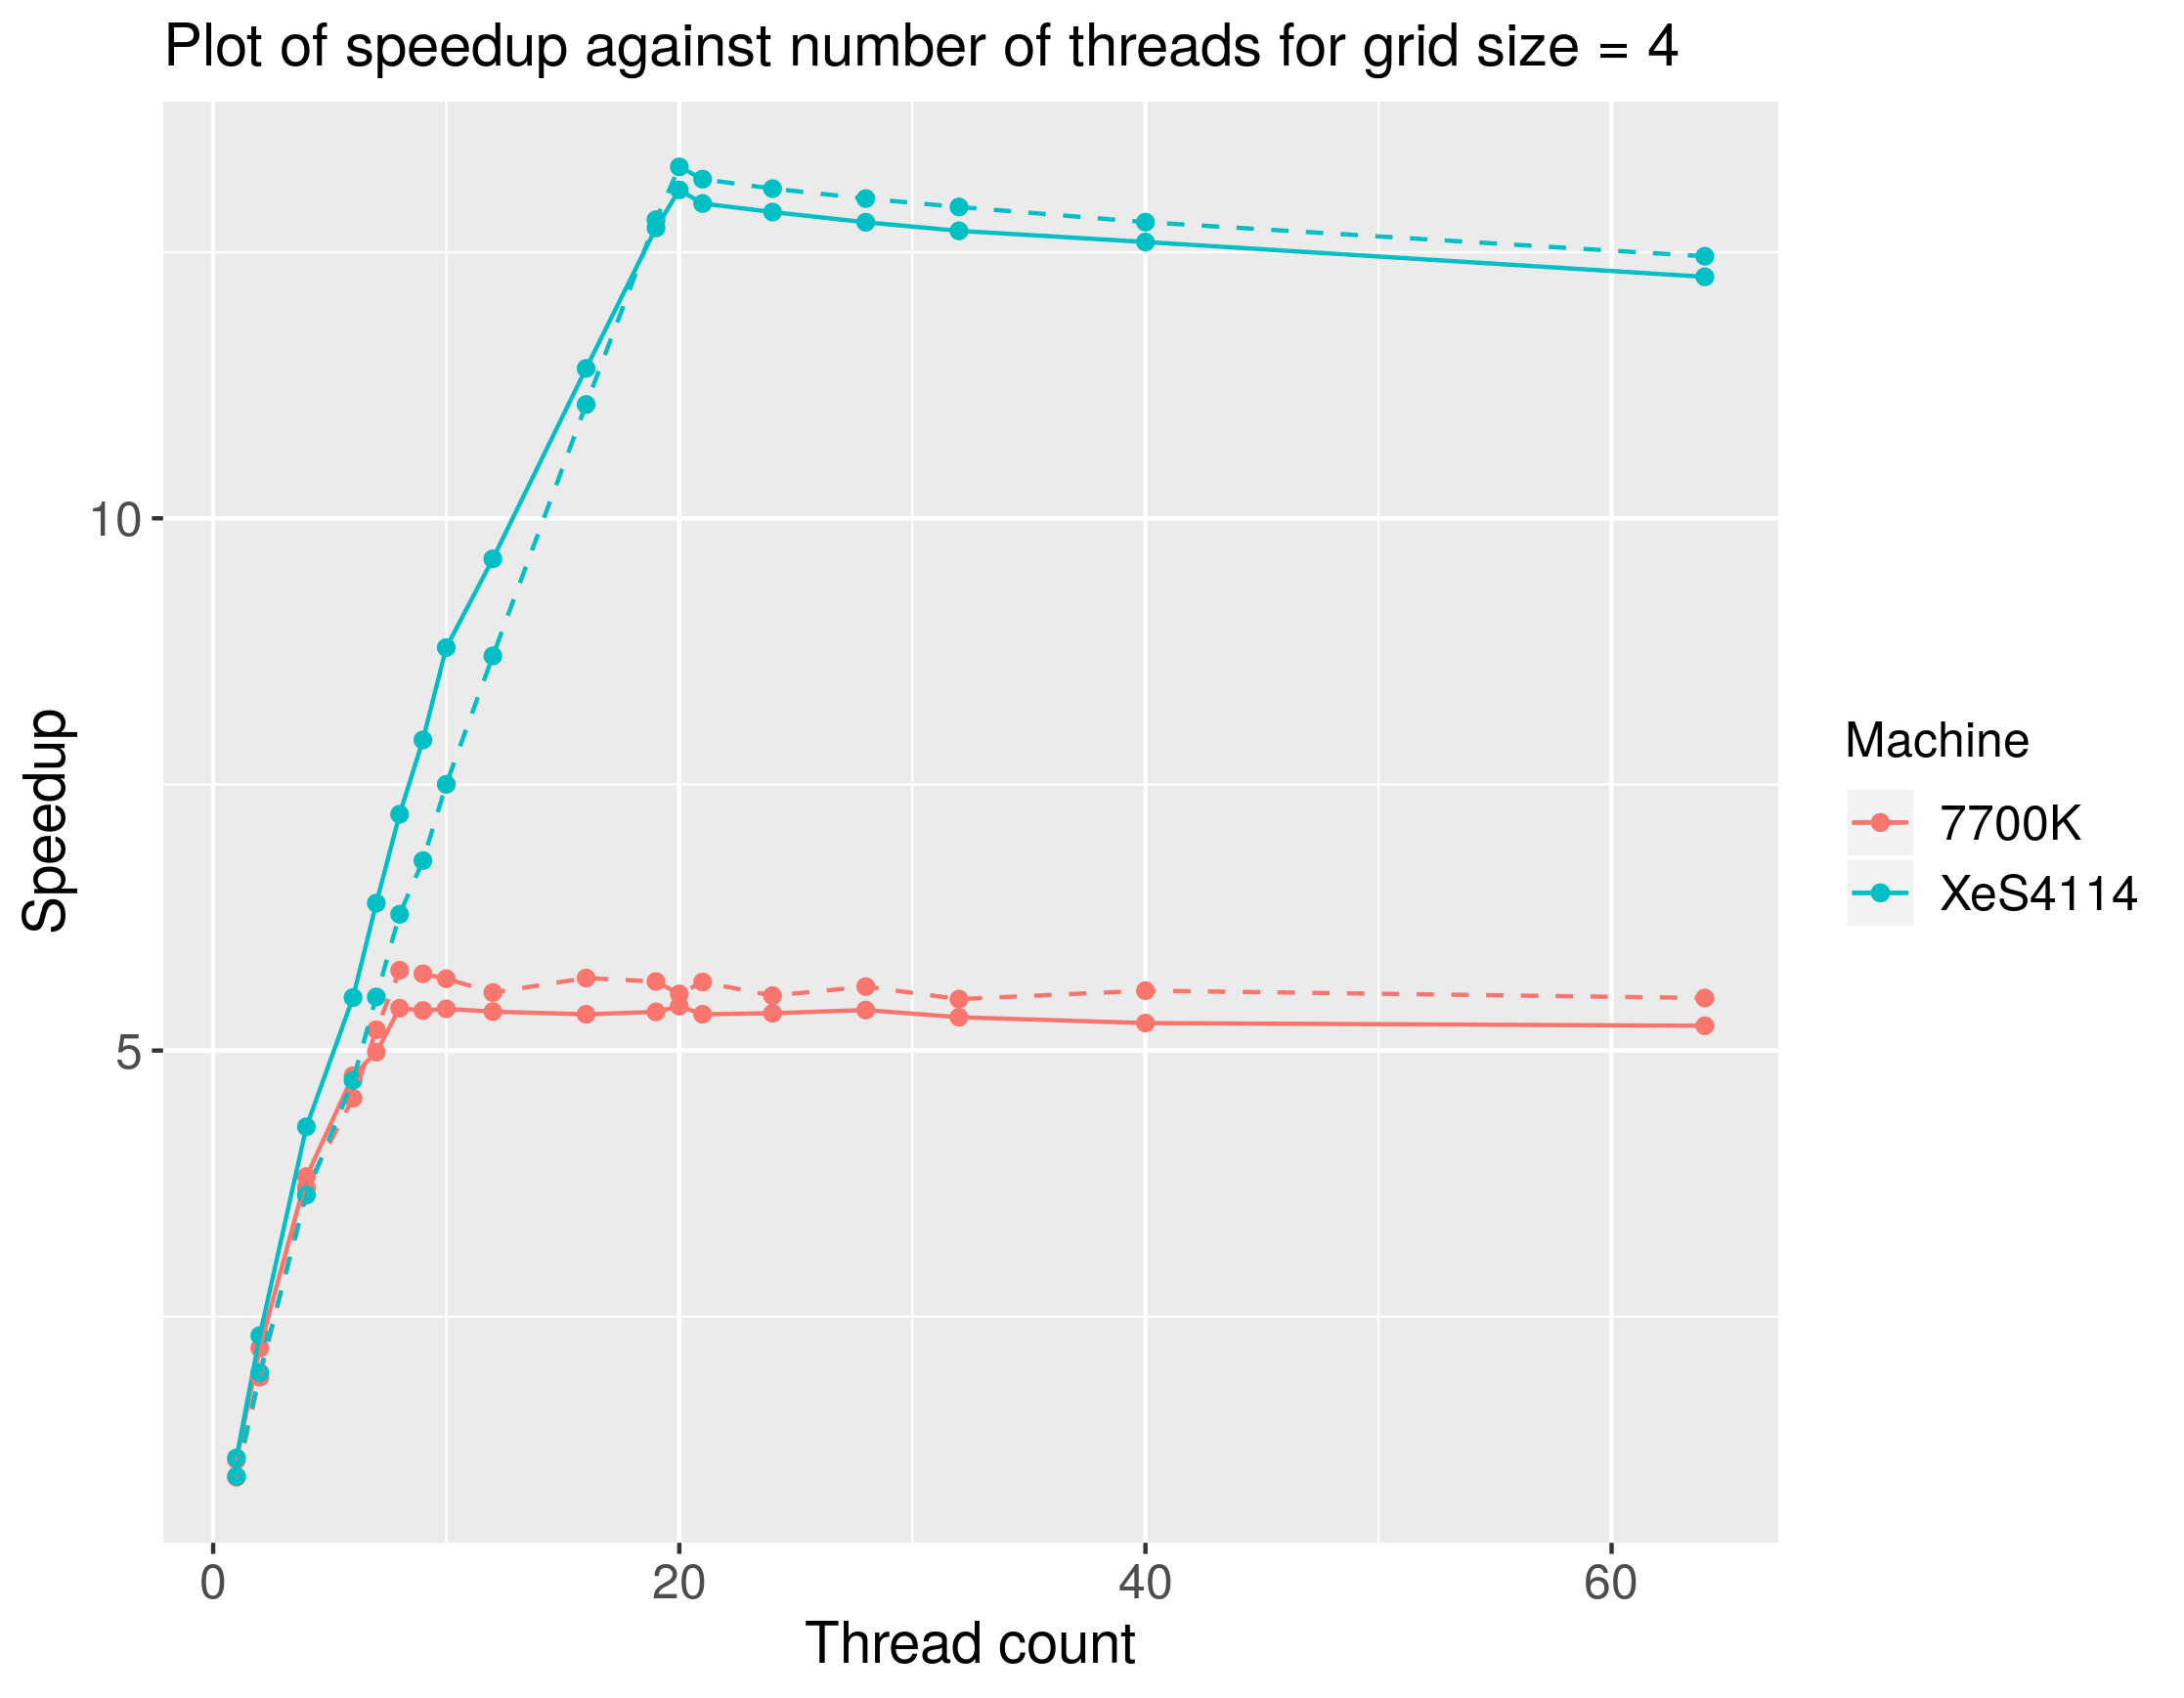
\includegraphics[width=0.75\textwidth]{optPar-gridSize4-speedup}
    \caption{Plot of speedup against number of threads $T$ for grid size of $G = 4$}
    \label{fig:optPar-gridSize4-speedup}
\end{figure}
\begin{figure}[H]
    \centering
    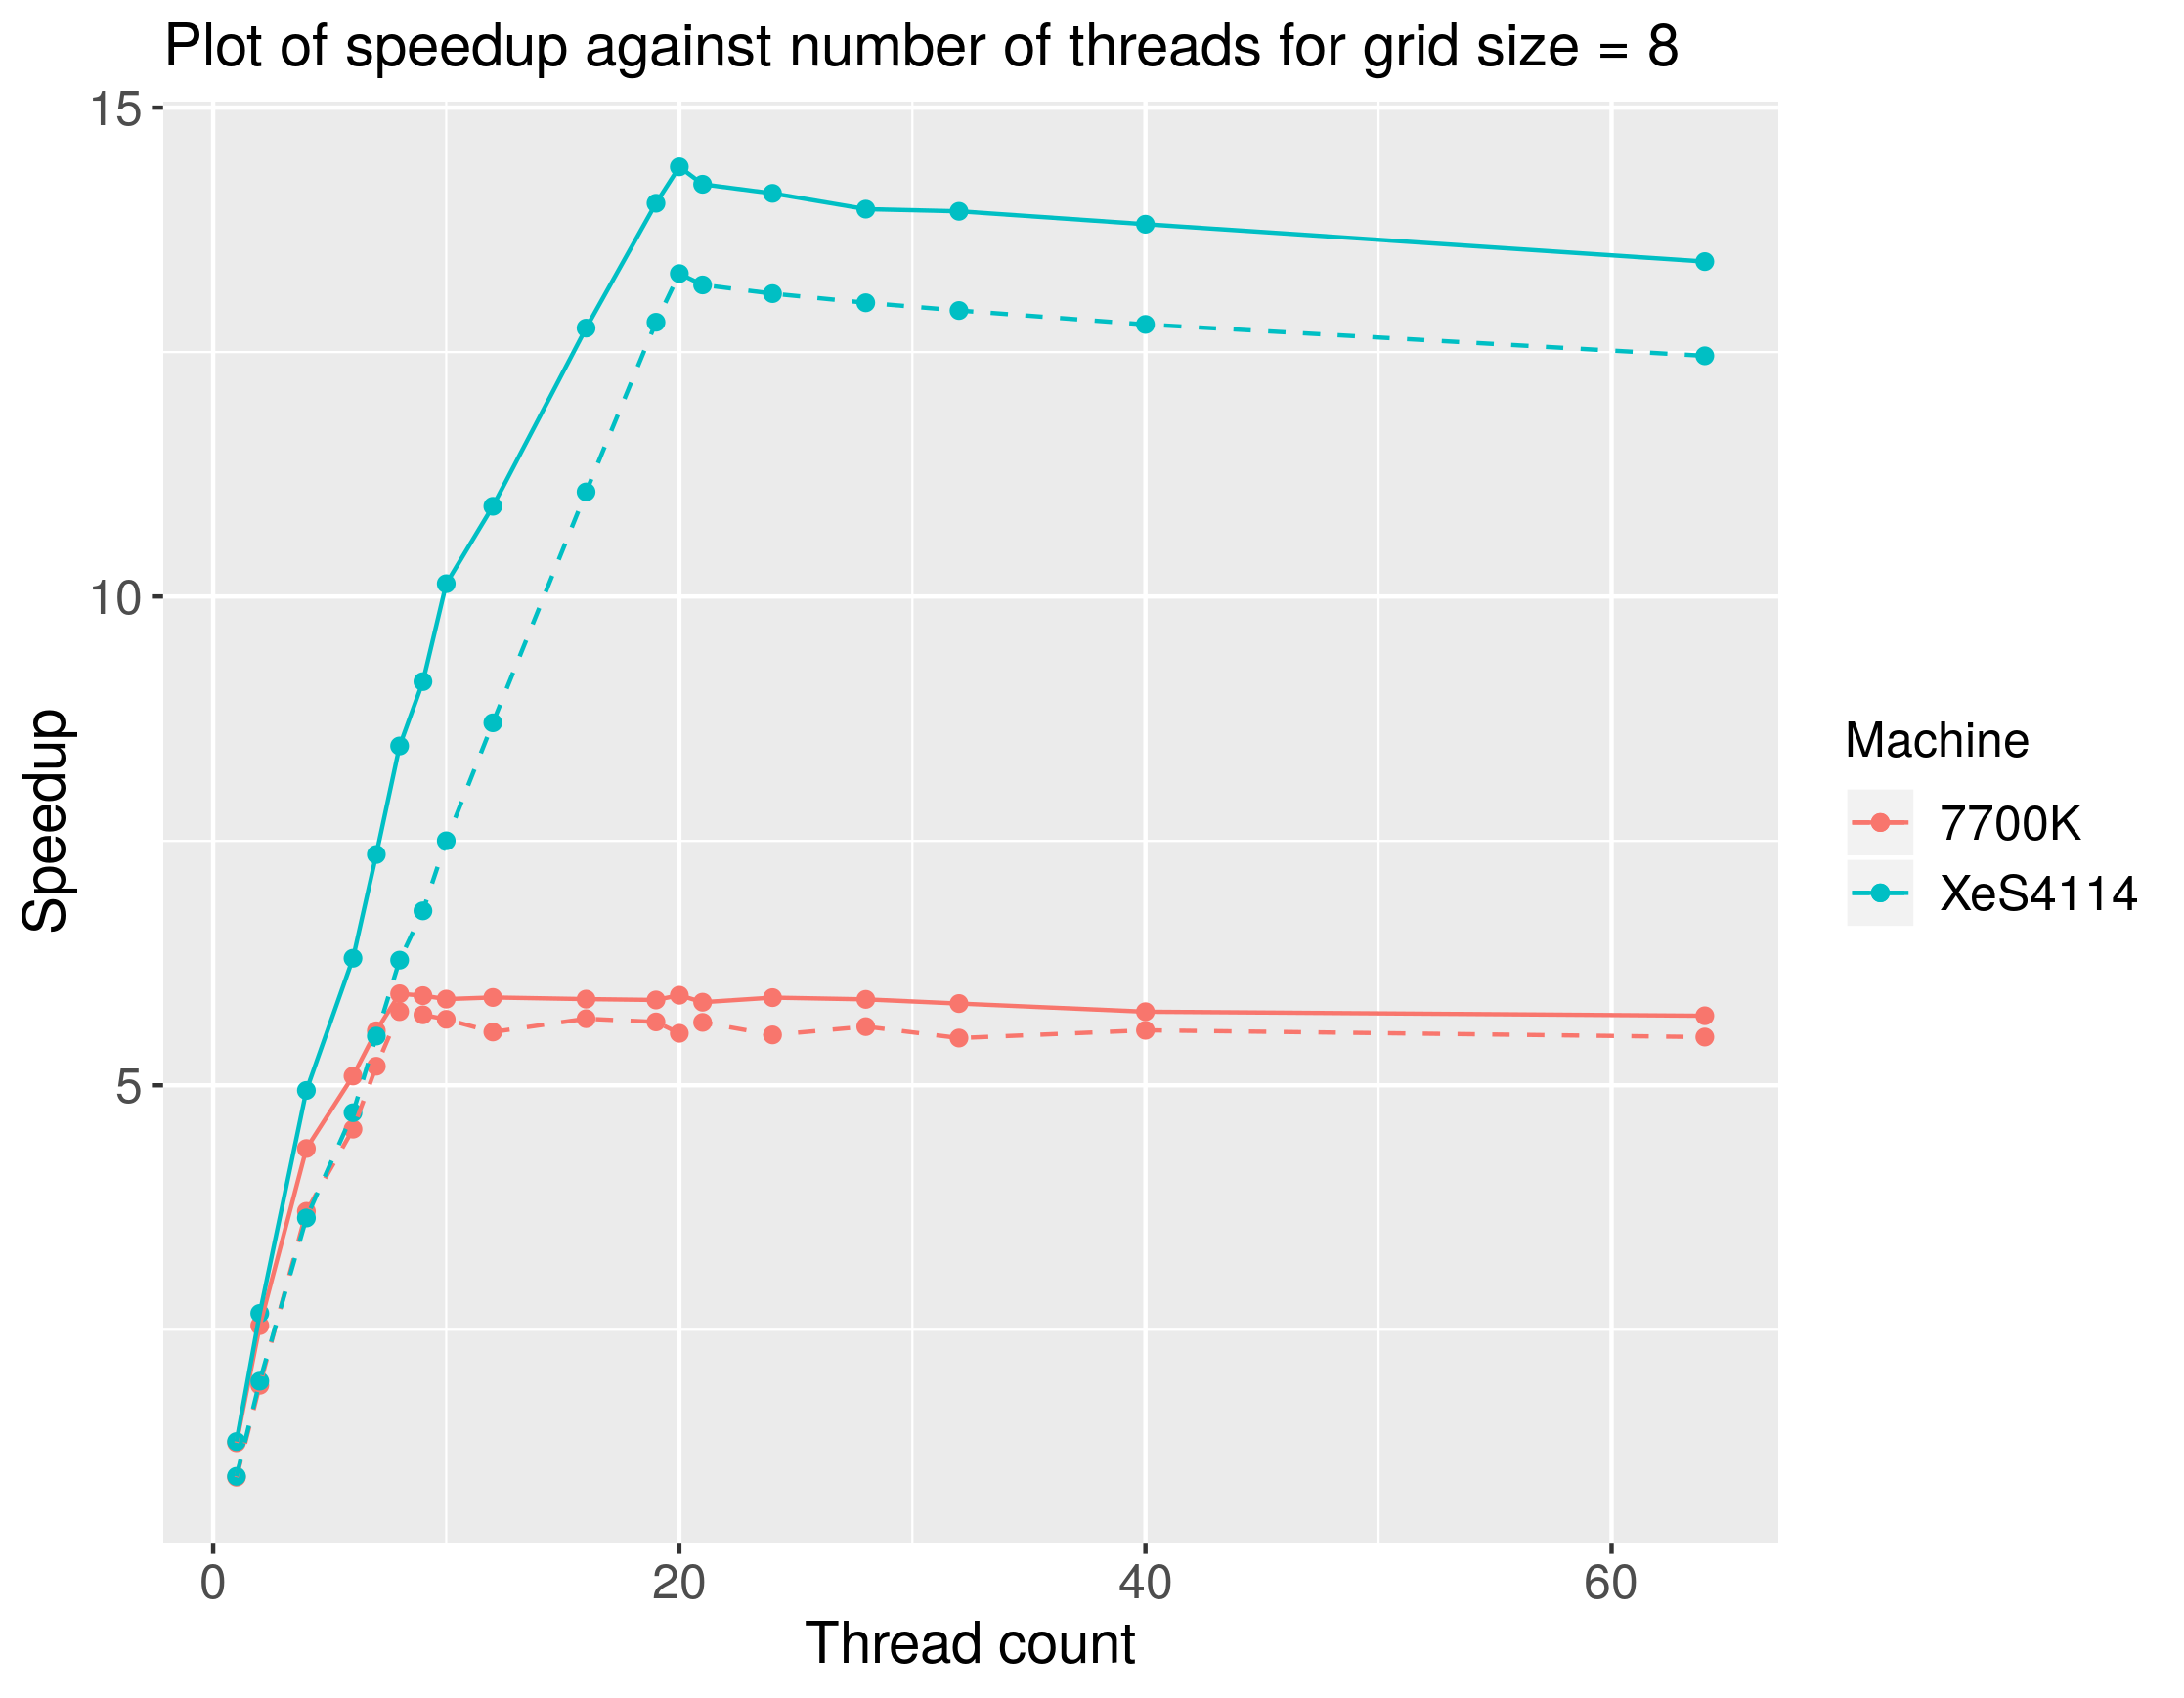
\includegraphics[width=0.75\textwidth]{optPar-gridSize8-speedup}
    \caption{Plot of speedup against number of threads $T$ for grid size of $G = 8$}
    \label{fig:optPar-gridSize8-speedup}
\end{figure}
\begin{figure}[H]
    \centering
    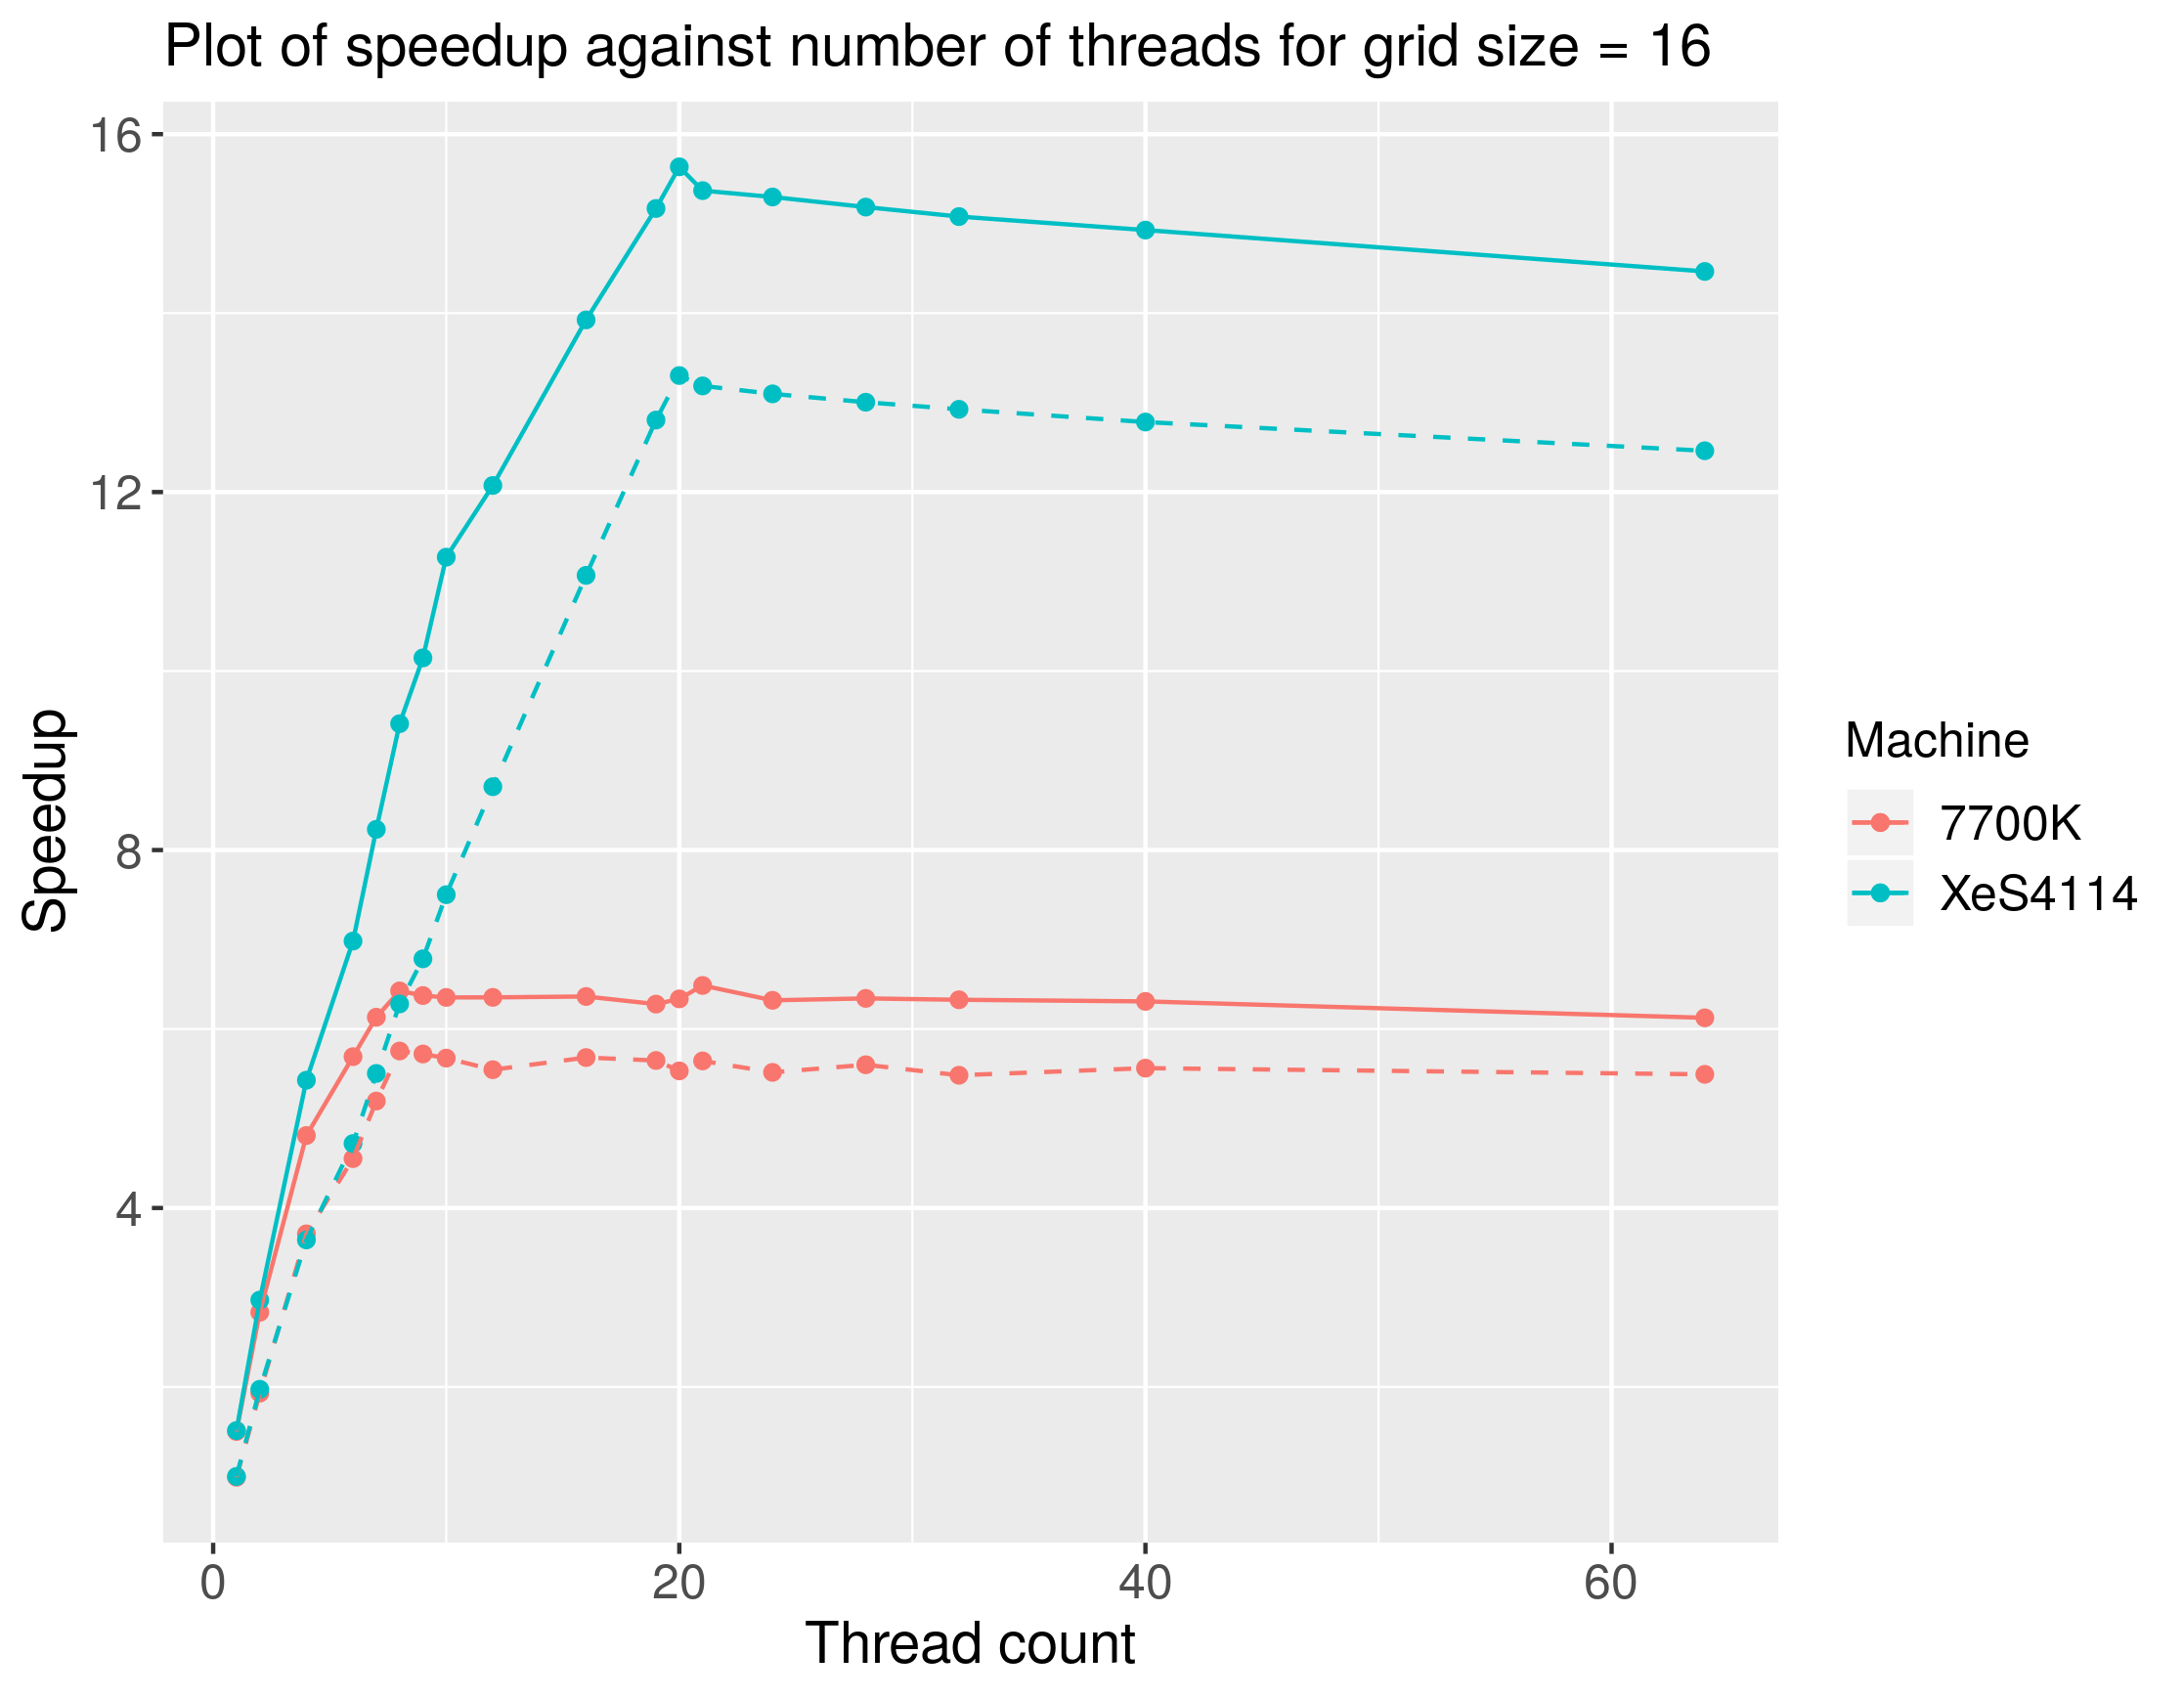
\includegraphics[width=0.75\textwidth]{optPar-gridSize16-speedup}
    \caption{Plot of speedup against number of threads $T$ for grid size of $G = 16$}
    \label{fig:optPar-gridSize16-speedup}
\end{figure}
\begin{figure}[H]
    \centering
    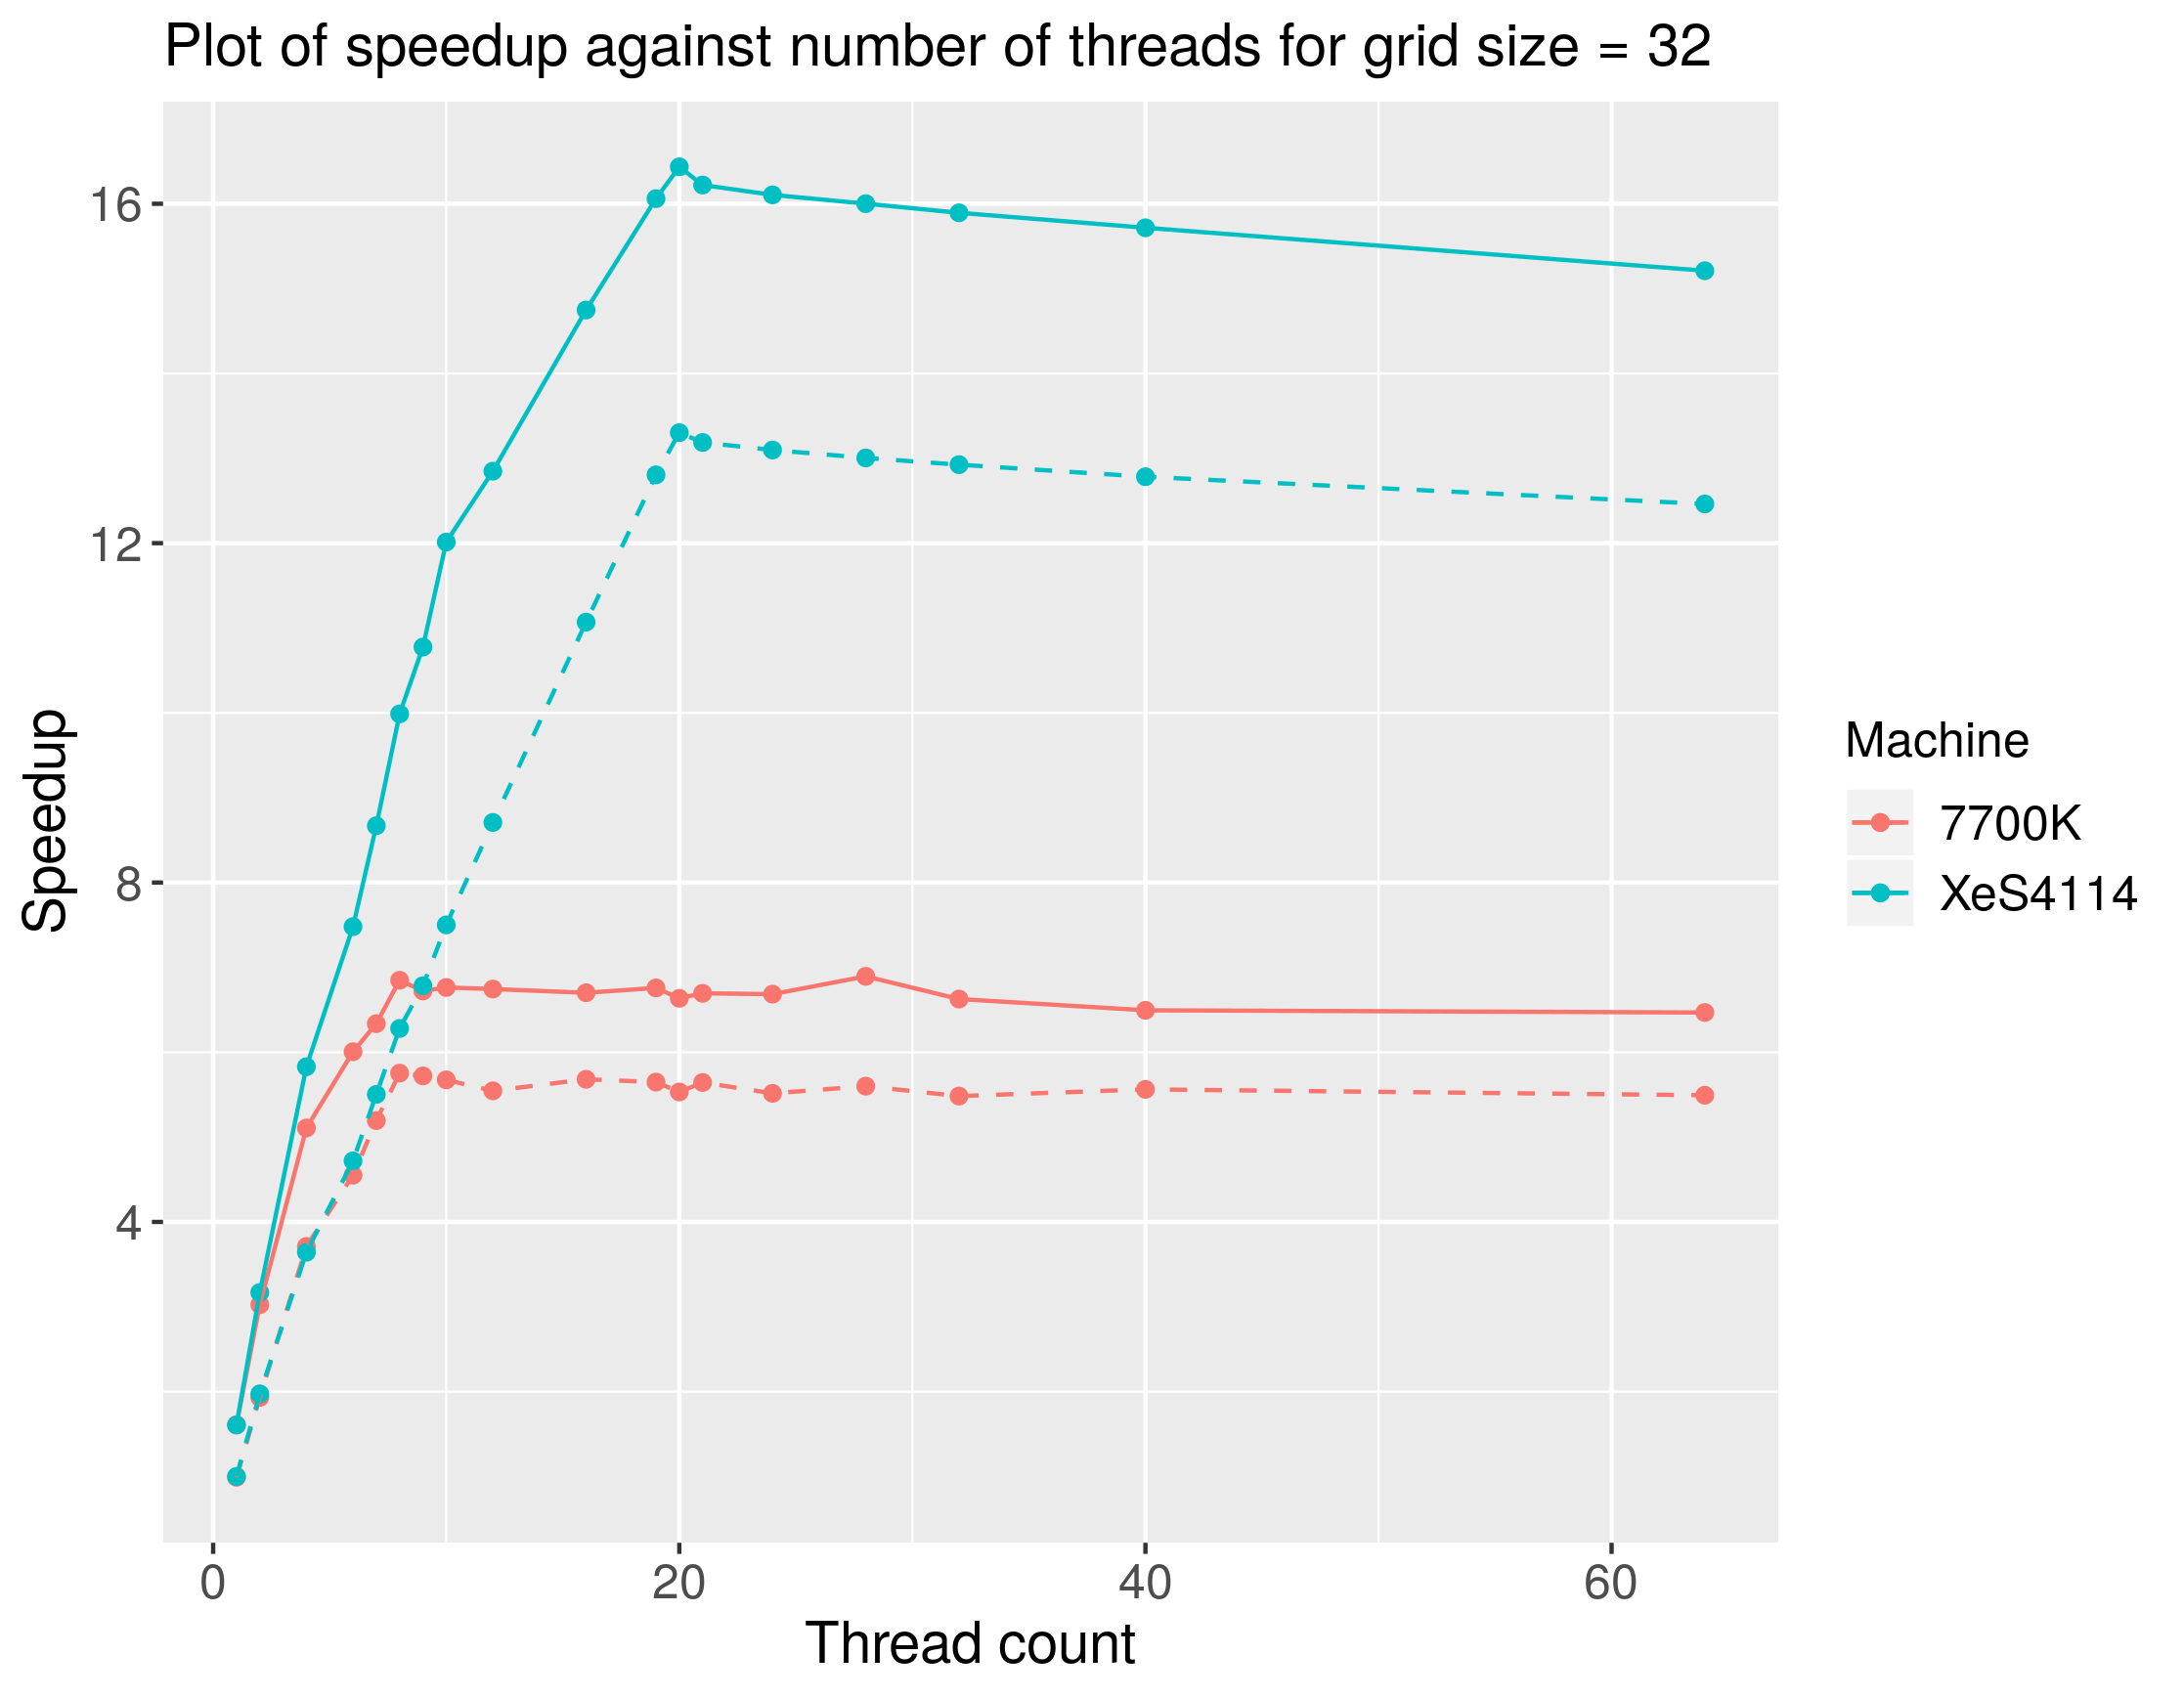
\includegraphics[width=0.75\textwidth]{optPar-gridSize32-speedup}
    \caption{Plot of speedup against number of threads $T$ for grid size of $G = 32$}
    \label{fig:optPar-gridSize32-speedup}
\end{figure}
\begin{figure}[H]
    \centering
    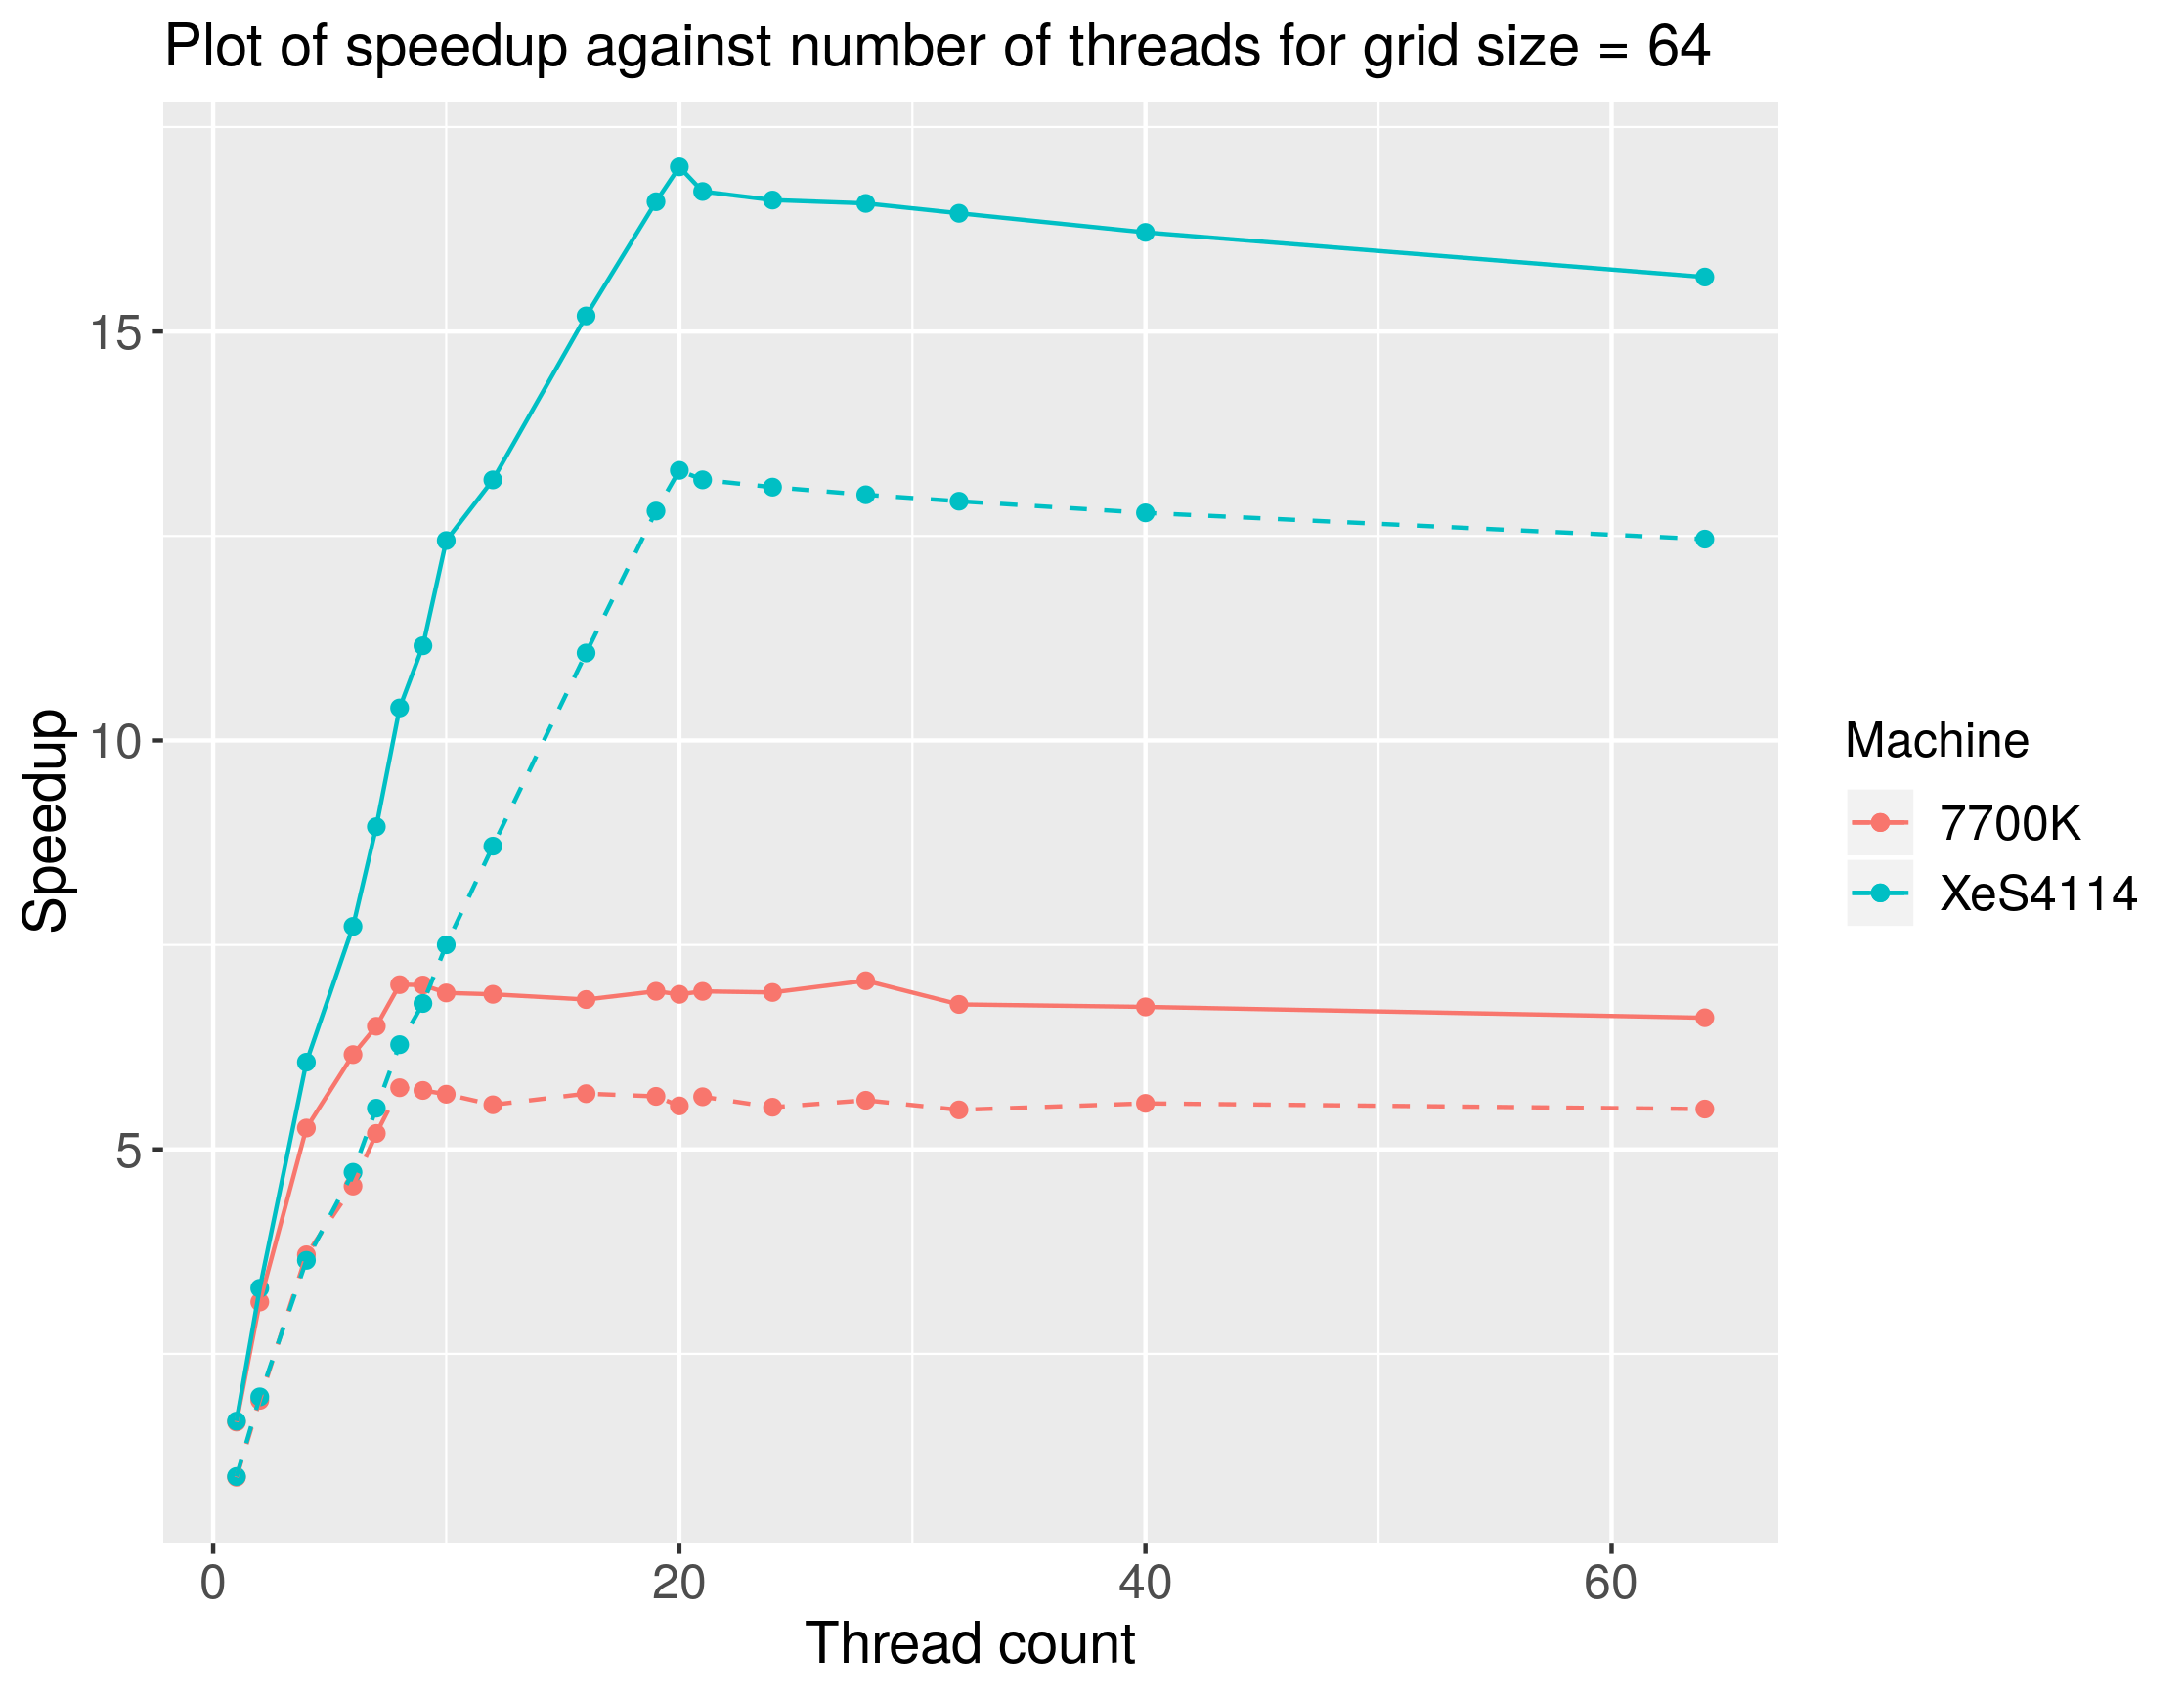
\includegraphics[width=0.75\textwidth]{optPar-gridSize64-speedup}
    \caption{Plot of speedup against number of threads $T$ for grid size of $G = 64$}
    \label{fig:optPar-gridSize64-speedup}
\end{figure}
\pagebreak

\section{Discussion: Early-pruning Parallel Implementation}

\subsection{Expectations}

As the new data was collected with the Bash script running in the background and ignoring the \texttt{SIGHUP} signal, we expect the significant degradation in execution time when $T$ is equal to the number of logical cores of the processor $T_{logical}$ to disappear. This should occur as there will no longer be contention for a CPU core by the process running the Bash script.

\subsection{Conclusions}

Figures \ref{fig:optPar-gridSize1-speedup} - \ref{fig:optPar-gridSize64-speedup} show the disappearance of the performance degradation when $T = T_{logical}$ for either processor, verifying our above hypothesis. \\

The plots show the optimal OpenMP thread count $T_{opt}$ (where the peak speedup was observed) has changed from the original dataset. \\

\begin{center} \begin{tabularx}{\textwidth} { | c | C | C | C | C | }
	\hline
	\multirow{2}{*}{$G$} & \multicolumn{2}{c|}{i7-7700K Optimal thread count $T_{opt}$} & \multicolumn{2}{c|}{Xeon 4114 Optimal thread count $T_{opt}$} \\
	\cline{2-5}
	& Parallel & Early-pruning & Parallel & Early-pruning \\ \hline
	1	&	\multirow{7}{*}{8}	&	8	&	\multirow{7}{*}{20}	&	20	\\
	\cline{1-1} \cline{3-3} \cline{5-5}
	2	&					&	9	&					&	20	\\
	\cline{1-1} \cline{3-3} \cline{5-5}
	4	&					&	20	&					&	20	\\
	\cline{1-1} \cline{3-3} \cline{5-5}
	8	&					&	8	&					&	20	\\
	\cline{1-1} \cline{3-3} \cline{5-5}
	16	&					&	21	&					&	20	\\
	\cline{1-1} \cline{3-3} \cline{5-5}
	32	&					&	28	&					&	20	\\
	\cline{1-1} \cline{3-3} \cline{5-5}
	64	&					&	28	&					&	20	\\
	\hline
\end{tabularx} \end{center}

For both processors, the speedup (regardless of implementation) increases with increasing thread count $T$ until $T_{logical}$, due to increasing parallelism. The speedup then typically peaks at $T_{opt} = T_{logical}$, afterwhich it exhibits a slow decrease due to increasing overhead from coordinating a larger number of OpenMP threads. \\

Interestingly, the early-pruning implementation deviates from this behaviour for the i7-7700K, where $T_{opt}$ appears to increase with $G$. This is possibly due to the increased number of branch misses from a finer grid (which rejects more particle-collision pairs). This results in a greater number of pipeline flushes that stall threads, allowing other threads to be switched in and increasing $T_{opt}$. \\

Figures \ref{fig:optPar-gridSize1-speedup} - \ref{fig:optPar-gridSize64-speedup} also demonstrates that the \textbf{peak speedup} $s_{peak}$ changes between the parallel and early parallel implementations, with the magnitude and direction of the change depending on the value of $G$. \\

\begin{center} \begin{tabularx}{\textwidth} { | c | c | C | C | c | C | C | } \hline
	\multirow{2}{*}{$G$} & \multicolumn{3}{c|}{i7-7700K Peak speedup $s_{peak}$} & \multicolumn{3}{c|}{Xeon 4114 Peak speedup $s_{peak}$} \\
	\cline{2-7}
	& Parallel & Early-pruning & Improvement & Parallel & Early-pruning & Improvement \\ \hline
	1	&	\multirow{7}{*}{5.754}	&	4.933	&	-14.27\%	&	\multirow{7}{*}{13.302}	&	11.969	&	-10.02\%	\\
	\cline{1-1} \cline{3-4} \cline{6-7}
	2	&						&	4.931	&	-14.30\%	&						&	11.971	&	-10.01\%	\\
	\cline{1-1} \cline{3-4} \cline{6-7}
	4	&						&	5.417	&	-5.86\%	&						&	13.086	&	-1.62\%	\\
	\cline{1-1} \cline{3-4} \cline{6-7}
	8	&						&	5.936	&	3.16\%	&						&	14.394	&	8.21\%	\\
	\cline{1-1} \cline{3-4} \cline{6-7}
	16	&						&	6.486	&	12.72\%	&						&	15.634	&	17.53\%	\\
	\cline{1-1} \cline{3-4} \cline{6-7}
	32	&						&	6.894	&	19.81\%	&						&	16.434	&	23.55\%	\\
	\cline{1-1} \cline{3-4} \cline{6-7}
	64	&						&	7.062	&	22.73\%	&						&	17.013	&	27.90\%	\\
	\hline
\end{tabularx} \end{center}

The table above shows that the improvement in speedup granted by the early-pruning optimisation increases with the grid size $G$, reaching a maximum of about $\sim25\%$. This is expected, since a finer grid (larger $G$) approximates the yellow region in Figure \ref{fig:chap8ExpandedSet} better, allowing a greater proportion of improbable particle-collision pairs to be pruned away. \\

At $G = 1$, the grid only contains one cell - the entire box, and thus computing the cell ID (trivially) for each particle for every time step incurs a significant penalty to the execution time and thus peak speedup. For $G = 2$, the penalty remains similar, since a $2\times2$ grid is too coarse and every cell within intersects some part of the collision circle of a particle, and thus no particles are pruned. \\

We see that the turnaround point for $G$, at which the penalty of computing the grid positions of particles is outweighed by the savings from pruned collision pairs, lies somewhere between $G = 4$ and $G = 8$. \\

From the trend above, we expect any further improvements beyond a grid size of $G = 64$ to diminish rapidly and approach some asymptotic value of the improvement, somewhere in the region of $\sim28\%$ for the i7-7700K and $\sim35\%$ for the Xeon 4114. \\

Overall, this optimisation has a significant effect on execution time, yet does not compromise correctness of the simulation.

\end{document}
